\documentclass[12pt, final]{article}

%_ PACKAGES __________________________________________________________________________ %

%__ INPUT/OUTPUT LANGUAGE _________________________________ %
\usepackage[portuguese,english]{babel}
\usepackage[utf8]{inputenc}
\usepackage[T1]{fontenc}
\usepackage{enumitem}
\usepackage{indentfirst}
\usepackage[super]{nth}
\usepackage{setspace}

%__ MATH __________________________________________________ %
\usepackage{amsfonts}
\usepackage{amssymb}
\usepackage{amsmath}
\usepackage{amsthm}
\usepackage{bbm}

%__ GRAPHS & TABLES________________________________________ %
\usepackage{graphicx}
\usepackage{booktabs}
\usepackage{multirow}
\usepackage{array}
\usepackage[flushleft,online,para]{threeparttable}
\usepackage{multirow}
\usepackage{svg}
\usepackage{pdfpages}
\usepackage{float}

% \usepackage[nolists,heads,tablesfirst,nomarkers]{endfloat}
% \renewcommand{\efloatseparator}{\mbox} % allows tables to share a page

\usepackage{sublabel}

\usepackage{caption}
\usepackage{subcaption}
\usepackage{chngcntr}

\usepackage{parskip}       

% \usepackage[capposition=top]{floatrow}


\usepackage{tabularx}
\newcolumntype{Z}{>{\centering\arraybackslash}X}
\newcolumntype{L}{>{\raggedright\arraybackslash}X}

\usepackage{dcolumn}
\newcolumntype{d}[1]{D{.}{.}{#1}}

\usepackage{rotating}               
\usepackage{lscape}
\usepackage{pdflscape}
% \DeclareDelayedFloatFlavor{sidewaystable}{table}

%__ BIBLIOGRAPHY __________________________________________ %
\usepackage[round,longnamesfirst,nonamebreak]{natbib}
\usepackage{microtype}
%\usepackage{url}

%__ PDF, DISPLAY & PRODUCTIVITY ___________________________ %
\usepackage{xcolor}
\definecolor{darkblue}{rgb}{0,0,0.5}
\usepackage{hyperref}
\hypersetup{
	colorlinks = true,
	linkcolor = darkblue,
	citecolor = darkblue,
	pdfborder = 0 0 0,
	pdfdisplaydoctitle = true,
	pdfhighlight = /N,
	pdfpagelayout = OneColumn,
	pdfpagemode = UseNone,
	pdfstartview = {FitH},
	pdfauthor = {{MS, RR \& DC}},
	pdftitle = {{Health \& Constitutional Spending Reform}},
	pdfsubject = {{}}
}
\hypersetup{urlcolor=blue}

\usepackage[textsize=footnotesize, colorinlistoftodos, textwidth=4cm, obeyDraft]{todonotes}

\usepackage{geometry}
\geometry{verbose,tmargin=2.54cm,bmargin=2.54cm,lmargin=2.54cm,rmargin=2.54cm}
\usepackage{setspace}
\onehalfspacing

\usepackage[bottom, multiple]{footmisc}

\usepackage{verbatim}
\usepackage[normalem]{ulem}
\usepackage{mathpazo}
\usepackage{lscape}

\usepackage{fancyhdr}
\pagestyle{fancy}
\fancyhf{}
\fancyfoot[R]{\thepage}
\renewcommand{\headrulewidth}{0pt}


%__ APPENDIX _____________________________________________ %
\usepackage[,titletoc,toc,title,page]{appendix}

%__ COMMANDS _________________________________________________________________________ %
\newcommand{\mc}{\multicolumn}
\newcommand{\lbar}{\underline}
\newcommand{\ubar}{\overline}

\usepackage{etoolbox}
\usepackage{tocloft}






\usepackage{etoolbox}
\usepackage{tocloft}


%\newcommand\aauthorA{Michel Szklo}
\newcommand\aaffiliationA{FGV-SP}

\begin{document}


\title{\textbf{Public Health Spending and Infant Mortality: Evidence from a Constitutional Reform in Brazil}}
\pagenumbering{gobble}

\author{
\small{Michel Szklo}\footnote{FGV - S\~ao Paulo School of Business Administration. Contact email: \href{mailto:mszklo@gmail.com}{mszklo@gmail.com}.}
\and \small{Damian Clarke}\footnote{Department of Economics, Universidad de Chile, MIPP \& IZA. Address: Diagonal Paraguay, 257, Santiago, Chile.  Contact email: \href{mailto:dclarke@fen.uchile.cl}{dclarke@fen.uchile.cl}.}
\and \small{Rudi Rocha}\footnote{FGV - S\~ao Paulo School of Business Administration, rudi.rocha@fgv.br.}
}
\date{\today}
\maketitle
\begin{center}
    %First draft: July 2020 \\
    %\emph{Preliminary. Please do not circulate}
\end{center}
\singlespacing
\begin{abstract}
 \noindent This paper treats Brazil as a case study to document the causal effects of health spending on infant mortality. By leveraging the variation in health spending promoted by Brazil's \nth{29} Constitutional Amendment of 2000, we are able to document not only the effects of health spending on infant mortality, but also the links in the chain connecting spending to health outcomes. We show that increases in health spending translate into greater primary care coverage, higher supply of hospitals and low skilled professionals. Associated with this effects we document moderate reductions in infant mortality within 24 hours and due to perinatal conditions, as well as long term reductions in total infant mortality, infant mortality amenable to primary care, and infant mortality by infectious and respiratory causes.  Our results contribute to the literature on the impacts of health spending by providing on of the first well identified causal parameter of the relationship between spending and mortality.
\end{abstract}

\noindent \textbf{JEL Codes}: I1, I3, O5\\
\noindent \textbf{Keywords}: Health spending; health care reform; health care production; infant mortality.

\newpage
%\thispagestyle{empty} 
%\onehalfspacing 
\setcounter{page}{1}



\section{Introduction}\label{sec:intro}
\pagenumbering{arabic}
\setstretch{1.5}
\setcounter{page}{1}


The last decades were marked by significant increases in public health expenditure around the globe. Data from the \cite{wb} reveals that per capita public health expenditure more than doubled since the turn of the century. A question that still remains unanswered is how effective this type of expenditure is in reducing mortality, specially among developing countries. 

Economist have been trying to answer this question for decades, but the evidence is still inconclusive. Moreover, most of the studies that attempt to establish this causal relationship are not able to analyse the links in the chain connecting health spending and health outcomes, and thus offer incomplete evidence on the effectiveness of public health spending.  

In this article, we aim to fill this gap by answering several questions along the chain connecting public health spending to health outcomes. How municipalities allocate resources when increasing health spending? How expenditures translate into health inputs, such as health infrastructure, health services, human resources and ambulatorial production? How all these affects infant mortality? To answer these questions we treat Brazil as case study, leveraging the variation in public health spending generated by Brazil's \nth{29} Constitutional Amendment of 2000 to document the causal effects of health spending on infant mortality using a difference-in-difference design with continuous treatment.

After a decade of public health underfinancing, in September of 2000, the Brazilian Congress enacted the \nth{29} Constitutional Amendment. It established the minimum share of resources that the federal, state and municipal governments need to spend on the provision of public health services. This institutional reform was responsible for increasing public health spending and for raising the direct participation of states and municipalities in the financing of health care \citep{Piola2013}.

Our econometric analysis ....

The remaining of the article is organized as follow: 


[Could add results on centralization.  Recent NBER WP showing that centralization is good for health, at least when considering obstetric care: \citet{Fischeretal2022}]

\section{Institutional Background}\label{sec:inst}
%\pagenumbering{arabic}
\setstretch{1.5}

The promulgation of the \citeyear{constituicao} Brazilian Federal Constitution (CF/1998) promoted profound changes in the provision of health care in Brazil as it established universal and egalitarian access to health care as a constitutional right. Under this context, the Unified Health System (\emph{Sistema Único de Saúde} -- SUS) was created to provide free and universal health care to all citizens. The CF/1988 also established that the provision of health care would be financed by the Social Security System budget, together with social assistance and the public pension system, with resources coming from the federal, state and municipal budgets, and specific tax instruments. The implementation of new social rights, in a period of hyperinflation and macroeconomic restrictions, led to several budget disputes and crisis in the financing of health care \citep{Piola2013}. In order to secure resources for the SUS, the \nth{29} Constitutional Amendment (\emph{Emenda Constitutional 29} -- EC/29) was enacted in September of 2000.

In August of 1999 the President of the Brazilian Lower House determined the attachment of two Constitutional Amendment Proposals (\emph{Proposta de Emenda Constitucional} - PEC) -- 169 of 1992 and 82 of 1995 -- into a new proposal. While the PEC/169 intended to secure 30\% of the federal Social Security budget to the provision of public health care and 10\% of state and municipalities tax income, the PEC/82 intended to secure all resources from taxes over profits and revenues, that were originally financing the whole Social Security budget, to the provision of health care. The new proposal was approved by the Lower House in November of 1999 and sent to the Upper House, where it was approved in September of 2000 as the EC/29.

The EC/29 established the minimum share of resources that the federal, state and municipal governments need to spend on the provision of public health services. According to Art. \nth{7} of EC/29, from 2000 to 2004, the federal government should spend in the year of 2000 the amount spent in 1999 increased in 5\% and from 2001 to 2004 correct this value by the GDP growth; the state governments should spend 12\% of its tax income net of transfers to municipal governments; and municipalities should spend 15\% of its tax income (own resource spending). The states and municipalities spending less than the amount established when the EC/29 was enacted would have to gradually increase its expenditure, decreasing the distance to the target by at least one fifth a year and spending at least 7\% of its tax income \footnote{The EC/29 established the shares of resources that governments needed to spend only until 2004. A Complementary Law would have to be approved to regulate the EC/29 from 2005 on. In the a absence of a Complementary Law the share of resources defined by the Art. \nth{7} would apply. The Complementary Law was only approved in 2012, but it made no changes to the Art. \nth{7}}. 

\begin{figure}[h!]
    \begin{center}
    \caption{\footnotesize Spending Density Plots}\label{fig:density}
    \begin{subfigure}{0.48\textwidth}
        \caption{\scriptsize Health Spending (\% of own resources)}\label{fig:density_a}
        \centering
        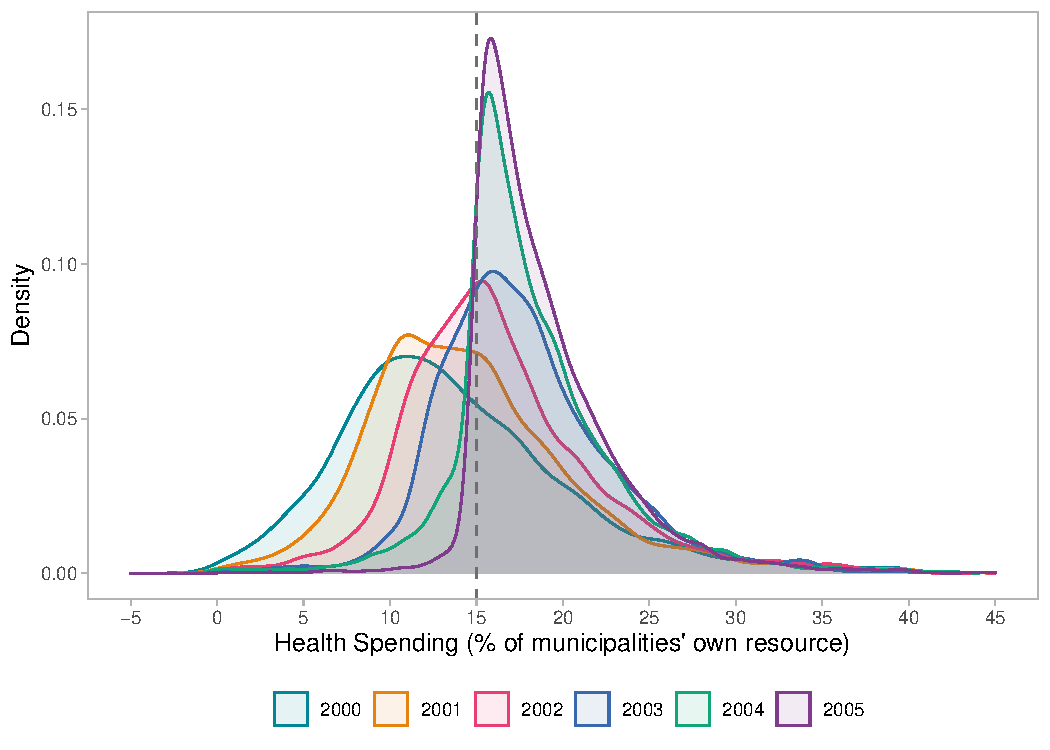
\includegraphics[width=\textwidth]{plots/hist_ec29.pdf}
    \end{subfigure}
        \begin{subfigure}{0.48\textwidth}
        \caption{\scriptsize Health Spending per capita (2010 R\$)}\label{fig:density_b}
        \centering
        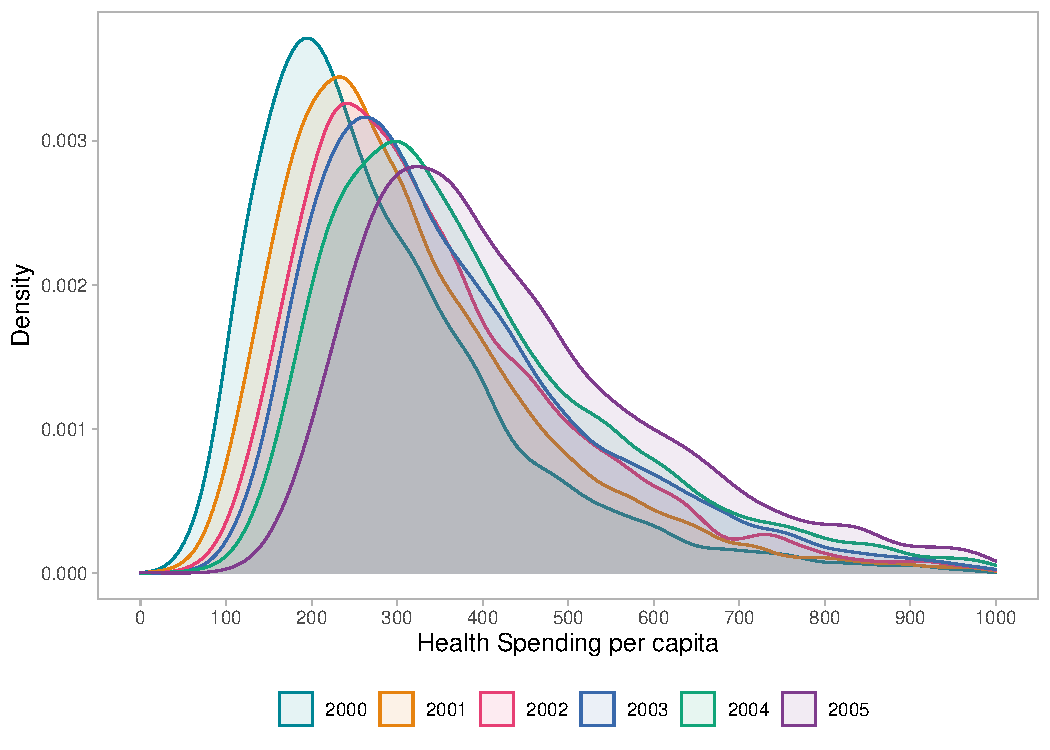
\includegraphics[width=\textwidth]{plots/hist_pc.pdf}
    \end{subfigure}
    \end{center}\vspace{+1pt}
    
    \floatfoot{    \scriptsize{Notes: Density plots calculated using SIOPS data (see Section \ref{sec:data} for more details). Dotted line in Figure \ref{fig:density_a} marks the EC/29 target (see Section \ref{sec:inst} for more details).}}

\end{figure}

\subsection{Municipalities Health Expenditure after the EC/29}

Figure \ref{fig:density_a} shows the distribution of municipalities according to their share of own resources spent in public health. While in 2000, our baseline year, most of the municipalities spent less than 15\%, in 2005 the great majority of municipalities were complying with the target stipulated by the EC/29. Figure \ref{fig:density_b} presents the distribution of municipalities according to their health spending per capita (in 2010 R\$). One could suggest two facts about this figure. First, there was a significant increase in the average health spending per capita and second, there was also some increase in the inequality of health spending per capita across municipalities.\footnote{\cite{Piola2013} highlights that the EC/29 provided a broad definition of health care that led some states and municipalities to include in this account expenditures that should not be considered part of expenditures related to the provision of public health services by the SUS.}


Figure \ref{fig:2} present trends in health spending at the municipality level converted into indices set at 100 in 2000, for the bottom and top quartile of the distribution of the share of own resources spent in health care. Figure \ref{fig:2a} shows that the municipalities in the bottom of the distribution presented much higher increase in health spending relative to the municipalities on the top of the distribution. Moreover, as shown in Figure \ref{fig:2b} and \ref{fig:2c}, expenditure coming from own resources explains almost all the difference in the health spending increase between the bottom and top quartile. Figure \ref{fig:3} plots trends for health spending per capita by source. Own resources has always been the main source of public health spending for municipalities, but the trends suggest that it gain even more importance after the EC/29 (Figure \ref{fig:3a}). In the baseline year of 2000, health spending per capita in the bottom quartile was half of the top quartile. Figures \ref{fig:3b} and \ref{fig:3b} suggest that all these difference comes from differential own resource spending. \cite{Piola2013} shows that states and municipalities own resource spending was responsible for about two thirds of the increase in health spending between 2000 and 2011.

\begin{figure}[h!]
    \begin{center}
    \caption{\footnotesize Health Spending Trends}\label{fig:2}
    \begin{subfigure}{.9\textwidth}
        \caption{\scriptsize Total Health Spending (2000 = 100)}\label{fig:2a}
        \centering
        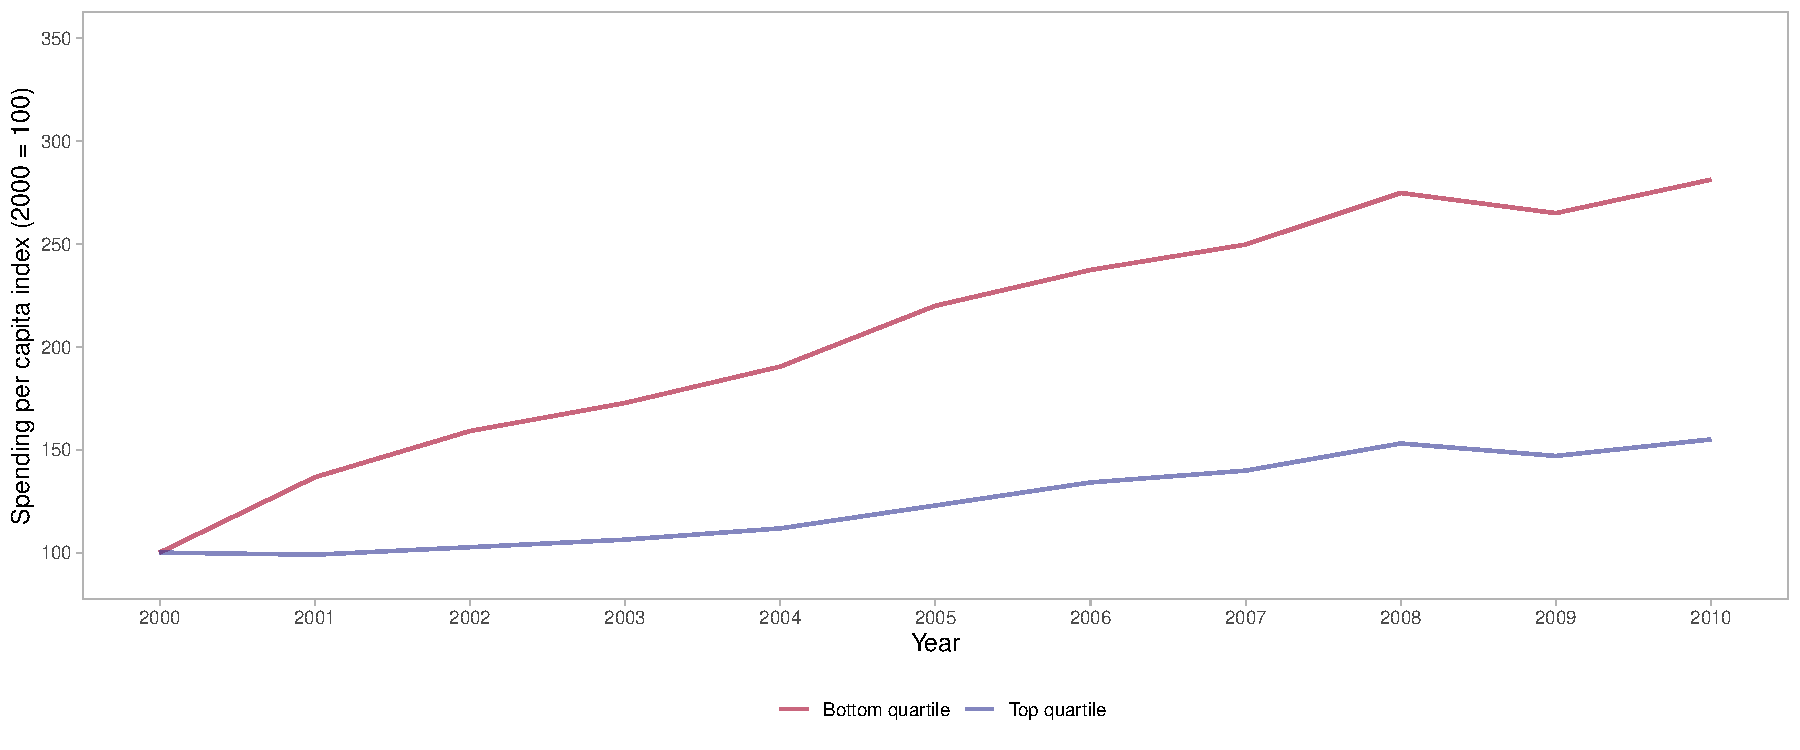
\includegraphics[width=\textwidth]{plots/plot_total.pdf}
    \end{subfigure}
        \begin{subfigure}{0.45\textwidth}
        \caption{\scriptsize Health Spending from Own Resources (2000 = 100)}\label{fig:2b}
        \centering
        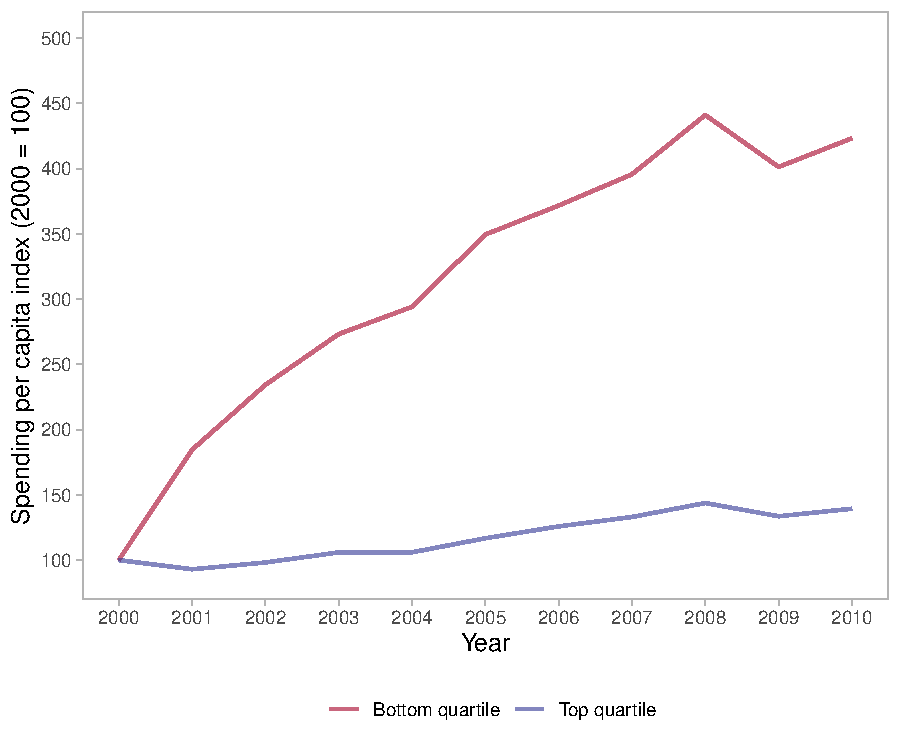
\includegraphics[width=\textwidth]{plots/plot_own.pdf}
    \end{subfigure}
        \begin{subfigure}{0.45\textwidth}
        \caption{\scriptsize Health Spending from Transfers (2000 = 100)}\label{fig:2c}
        \centering
        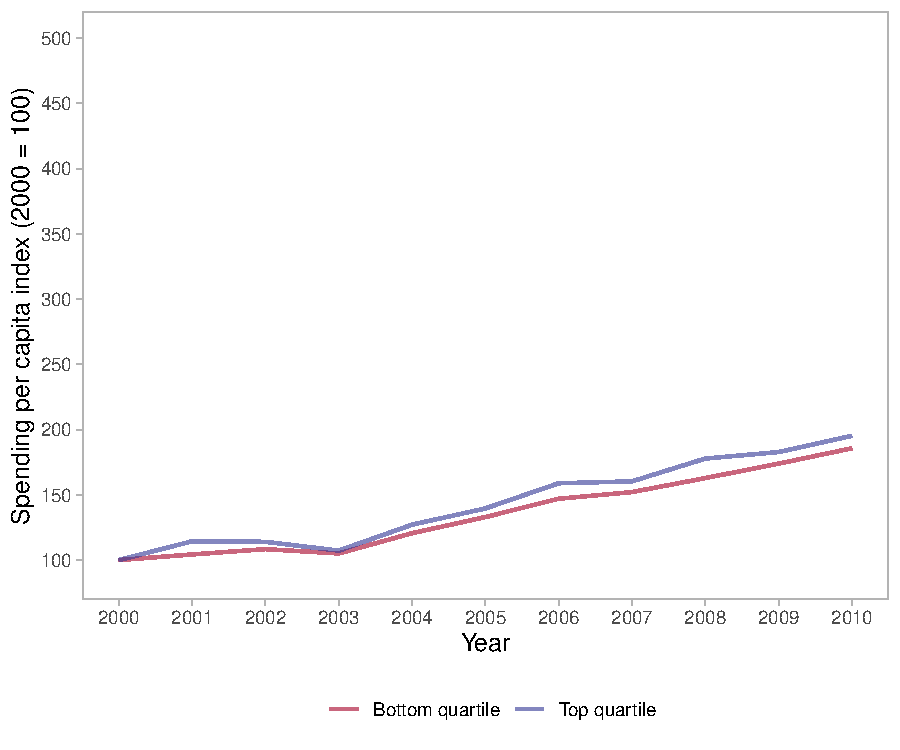
\includegraphics[width=\textwidth]{plots/plot_transf.pdf}
    \end{subfigure}
    \end{center}\vspace{+1pt}
\end{figure}
\begin{figure}[h!]
    \begin{center}
    \caption{\footnotesize Health Spending Trends}\label{fig:3}
    \begin{subfigure}{.9\textwidth}
        \caption{\scriptsize Health Spending by Source (R\$2010) - Full Sample}\label{fig:3a}
        \centering
        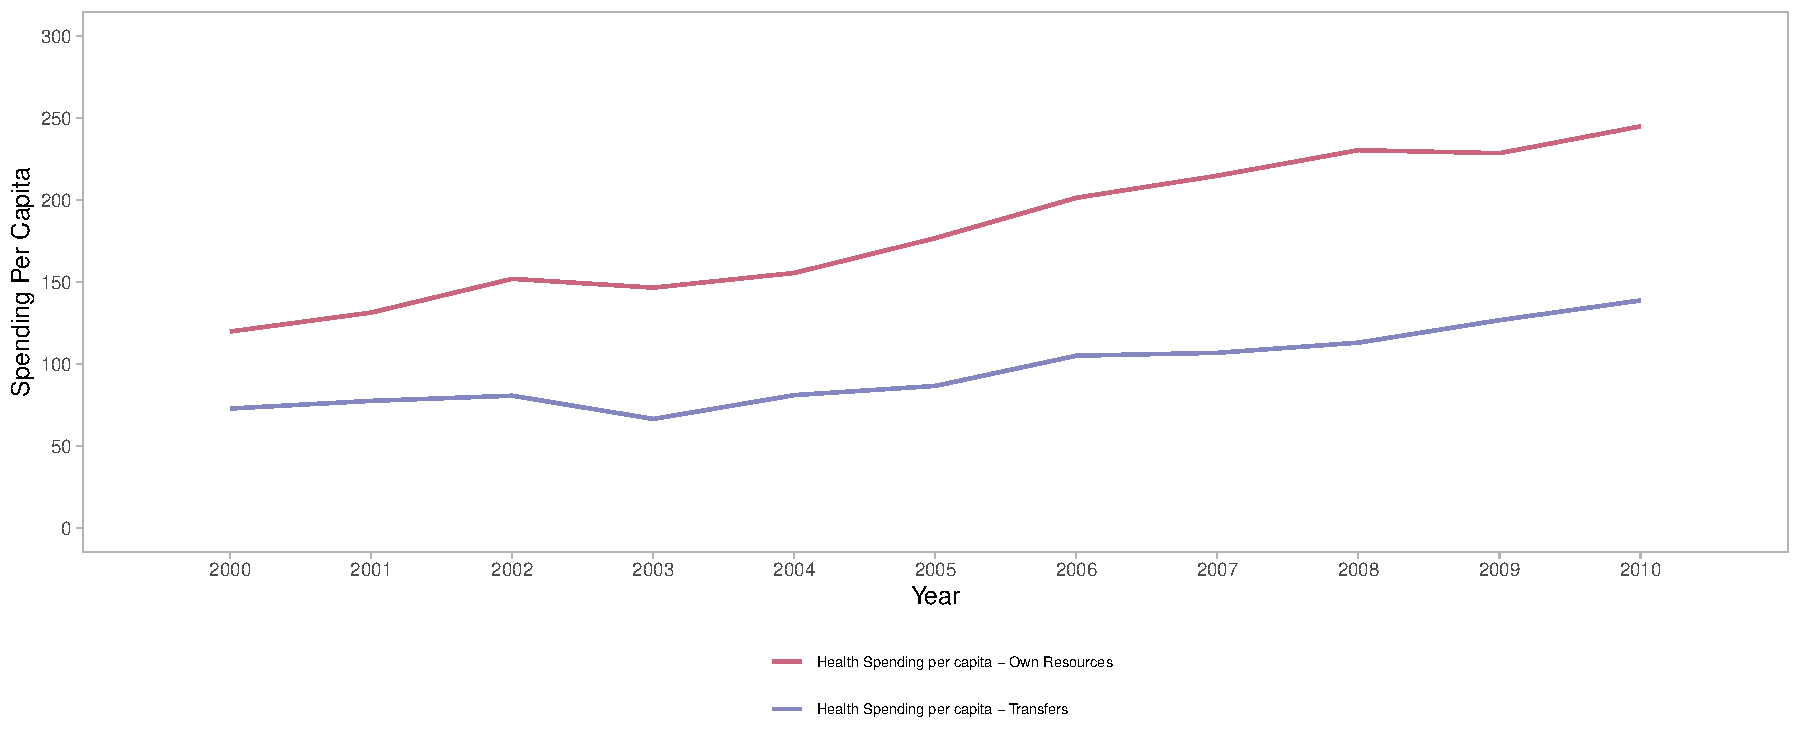
\includegraphics[width=\textwidth]{plots/plot_siops_level_source.pdf}
    \end{subfigure}
        \begin{subfigure}{0.45\textwidth}
        \caption{\scriptsize Health Spending by Source (R\$2010) - Bottom Quartile}\label{fig:3b}
        \centering
        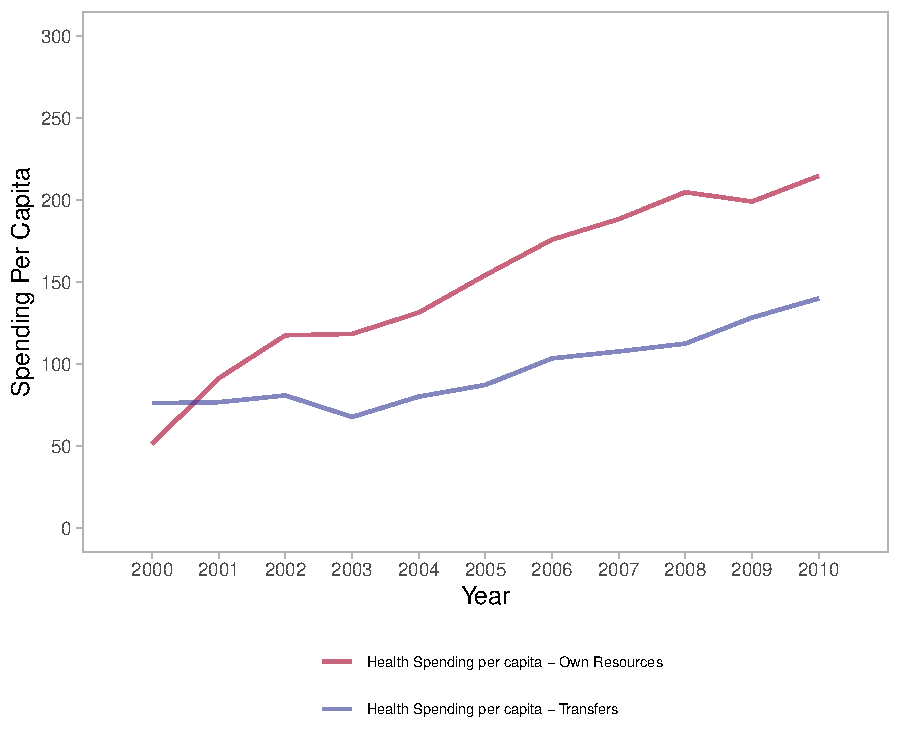
\includegraphics[width=\textwidth]{plots/plot_siops_level_source_bottom.pdf}
    \end{subfigure}
        \begin{subfigure}{0.45\textwidth}
        \caption{\scriptsize Health Spending by Source (R\$2010) - Top Quartile)}\label{fig:3c}
        \centering
        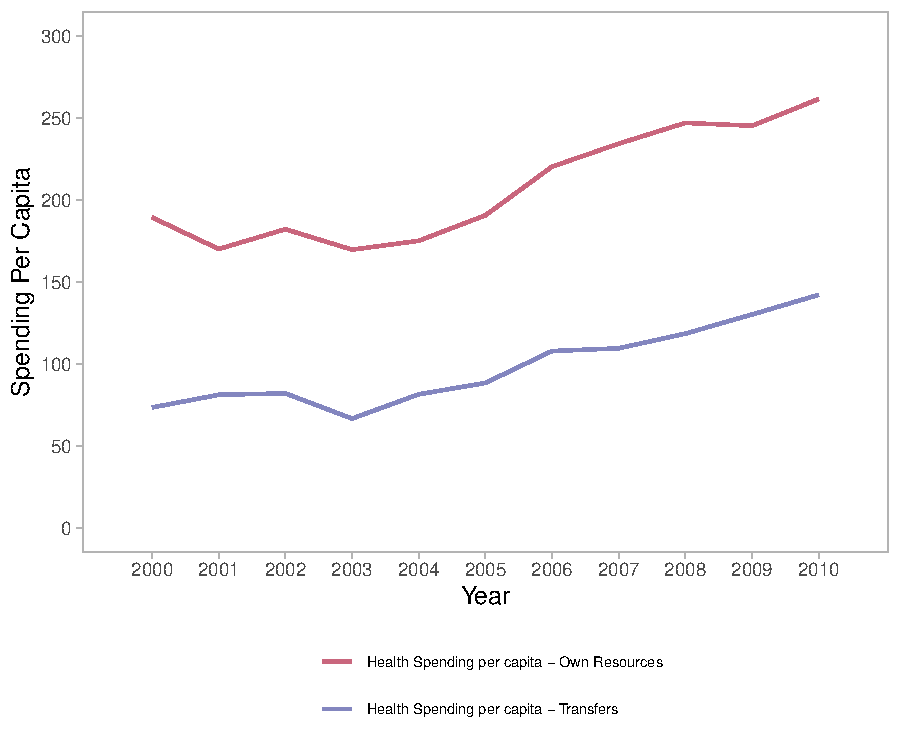
\includegraphics[width=\textwidth]{plots/plot_siops_level_source_top.pdf}
    \end{subfigure}
    \end{center}\vspace{+1pt}
    \scriptsize{Notes: Trends calculated using SIOPS spending data (see Section \ref{sec:data} for more details).}
\end{figure}


Moreover, municipalities' baseline level of own resource spending in health presents ample variation and is somewhat predictive of the change in total health spending per capita, which will be crucial to our identification strategy. Figure \ref{fig:4} plots, for all municipalities, the distance in percentage points to the EC/29 own resource spending target\footnote{We choose to work with the distance the target instead of the share of own resource expenditure in health in order to have easier to interpret estimates, as this measures presents a positive correlation with health spending} versus the change in total health spending per capita between 2000 and 2005. Consistently with the evidence presented in figure \ref{fig:2} and \ref{fig:3}, increases in health spending were larger in places with initially low levels of own resource spending, with a moderate to strong correlation of $0.45$.


\begin{figure}[h!]
\begin{center}
    \caption{Changes in Health Spending per capita (2000-2005)}
    \scalebox{0.7}{
    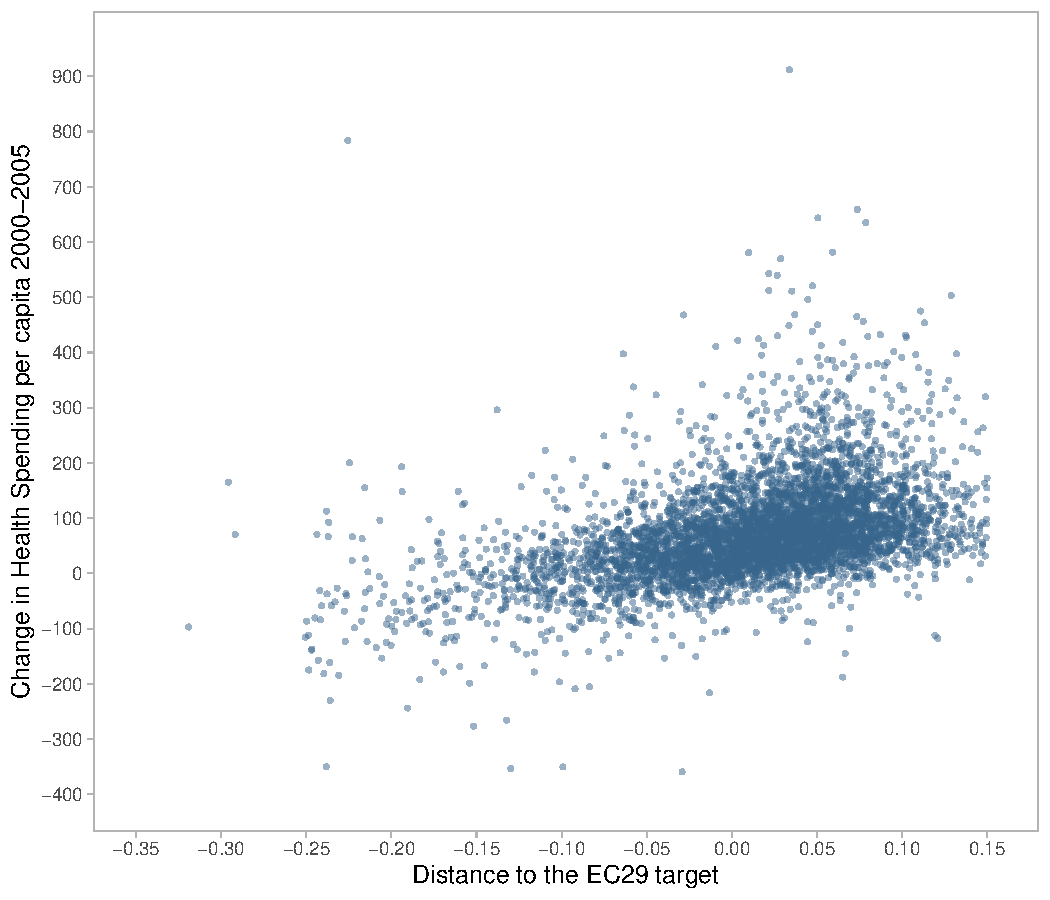
\includegraphics{plots/scatter_dist_ec29_baseline_change05.pdf}
    \label{fig:4}
    }
\end{center}
\end{figure}


In general, the descriptive evidence suggests that the EC/29 was responsible for bringing more resources to the provision of public health services and increasing the direct participation of states and municipalities in the financing of health care.

\section{Data}\label{sec:data}
\setstretch{1.5}

Table \ref{table:stats} presents summary statistics at the baseline year for all the variables used in this analysis: variables related to the EC/29, fiscal data, health inputs, infant mortality rates, birth outcomes, and control variables.

\subsection{EC/29 and Fiscal Data}

To evaluate municipalities' fiscal reactions to the EC/29, we combine public spending data from the Brazilian Finance System (FINBRA)\footnote{All spending data is presented in 2010 R\$. We used the General Price Index (IGP) to correct values}, which covers the period of 1998 to 2010, with data from the Brazilian National System of Public Health Budget (Datasus/SIOPS)\footnote{SIOPS was created right after the EC/29 to monitor revenues and expenditure in the provision of health care at the state and municipal levels, and to monitor compliance with the EC/29.} available from 2000 onward. FINBRA provides data on total public spending, and spending by a few aggregated categories, such as Health and Sanitation, Education and Culture, etc, and data on public revenues. The SIOPS, on the other hand, provides more detailed information on public health spending, which allow us to evaluate how municipalities allocate resources within the public health sector. It gathers data on total health spending, health spending from own resources, health spending from intergovernmental transfers, and health spending by types of spending, including spending in human resources, investments, services from third parties, and others\footnote{Others expenditures includes mainly administrative spending}. Moreover, SIOPS calculates for each municipality the share of own resources spent in the provision of health care, that we use to build our independent variable.

Figure \ref{fig:5} displays the spatial variation in the share of own resources spent in health. Municipalities below the EC/29 are represented with colors in the red scale, while municipalities above the target are represented with the blue scale. The map shows significant differences in the share of own resources spent in health within the same state, providing the identifying variation of this study as we include state fixed-effects in our main specification. 

\begin{figure}[h!]
\begin{center}
    \caption{EC/29 Compliance Geographic Variation}
    \scalebox{0.7}{
    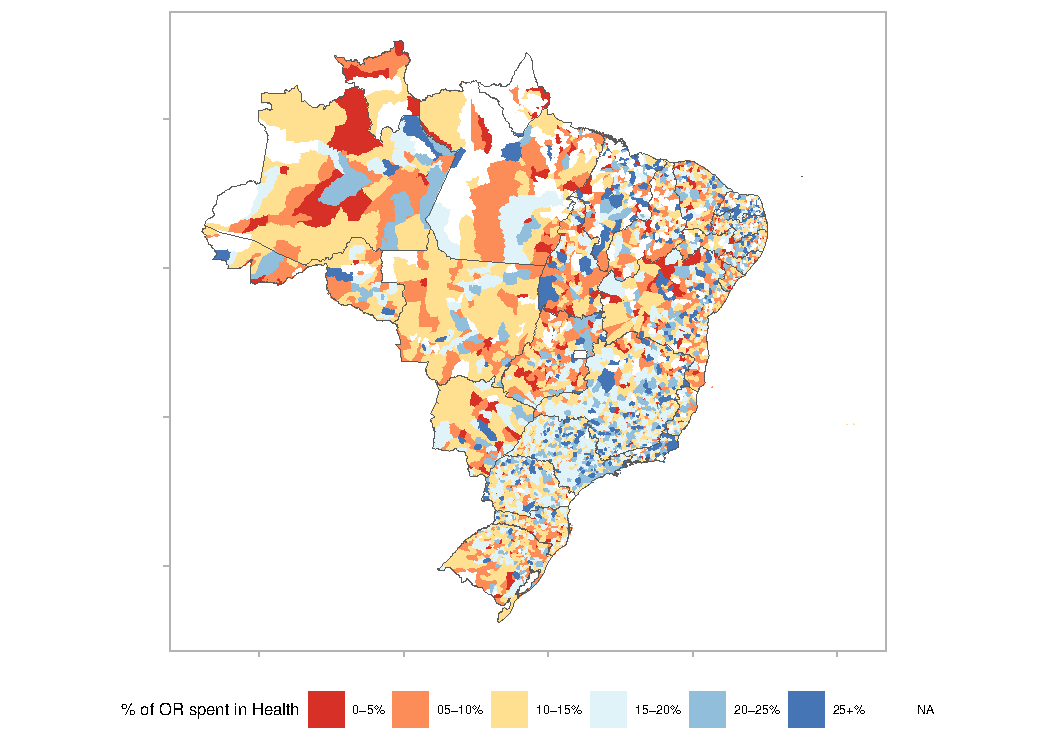
\includegraphics{plots/ec29_map.pdf}
    \label{fig:5}
    }
\end{center}
\end{figure}

\subsection{Health Inputs}

We combine data from several sources to build our health inputs data base. First we collect data on primary care coverage - extensive and intensive margin -  from Brazilian National System of Information on Primary Care (Datasus/SIAB) . Data on health human resources and hospital infrastructure comes from the 1999, 2002, 2005 and 2009 Medical-Sanitary Assistance Survey (AMS), a census of the health sector run by Brazilian Institute of Geography and Statistics (IBGE). 

The Brazilian National System of Information on Ambulatory Care (Datasus/SIA) every ambulatory procedure funded by SUS, with information on the type and complexity of the procedure, the health professional responsible, and the corresponding health facility register number. This data is used to create variables on ambulatory production, primary care ambulatory production, and ambulatory production by procedures complexity. We also use this data to indirectly create variables that measure the supply of health ambulatory facilities, as well as the supply of ambulatory facilities with health professionals related to primary care services. This is done by evaluating the number of facilities within a municipality that recorded ambulatory procedures of interests or ambulatory procedures executed by specific professionals of interest \footnote{We are able to construct these variables only for the period of 1998 to 2007, as changes in the SIA classification of ambulatorial procedures changes in 2008.}.

To measure access to health services, we used data from the from Brazilian National System of Birth Records (Datasus/SINASC), that records every birth in Brazil and provides detailed information on these births. Using this data we calculated the share of no prenatal visits, 1-6 prenatal visits and more than 7 prenatal visits. Importantly, in the first years of our sample, there is no information on prenatal visits for a considerable amount of births. To account for this under-registration issue, we also calculated the share of prenatal ignored. By estimating the impacts on this variable, we can separate the effects of access increasing from improvements in data registration.


\subsection{Infant Mortality and Birth Outcomes}

We use micro-data from Brazilian National System of Mortality Records (Datasus/SIM) and from SINASC to construct Infant Mortality Rates. These micro-data allow us to construct Infant Mortality Rates by the timing of death, and for the main causes of death. Moreover, following \cite{alfradique2009internaccoes} classification we are able to construct mortality rates that are amenable and non-amenable to primary care access. The SINASC also provides detailed information on Apgar 1 and 5, birth weight, and premature births. We also use data on population by age and sex from Datasus to calculate fertility rates.


\subsection{Controls}

Our control variables can be classified into three different categories: baseline socioeconomic controls, time varying socioeconomic controls, and time varying fiscal controls. The first, comes from IBGE's Census of 2000. Our time varying socioeconomic controls includes GDP per capita, from IBGE, and the \emph{Bolsa Família} program transfers per capita, from the Ministry of Social Development. The last set of controls comes from FINBRA dataset. We use as fiscal controls the average health spending per capita in the bordering municipalities\footnote{\cite{castro2021effects} show the importance spending of spillover effects in health, which highlights the importance of including this control.} and the share of total current public revenue spent with personnel\footnote{In the year of 2000, the Fiscal Responsibility Law \citep{lrf} was enacted. This law defined that municipalities cannot spend more than 60\% of its revenue in personnel. We include this control to account for the different incentives municipalities might face according to their compliance with the law.}. 

\section{Empirical Approach}\label{sec:emp}
\setstretch{1.5}

We estimate the effects of the EC/29 using a difference-in-difference (DiD) design with a continuous treatment, exploiting within-municipality variation. Intuitively, we compare the evolution of outcomes in municipalities far from the EC/29 15\% target with municipalities that were already complying with the target. The underlying assumption is that changes in outcomes for the later group provide a good counterfactual for changes that would have been observed in the former group had they been complying with the target. 

The identification relies on the cross-municipality variation in the share of own resource spent in the provision of healthcare and on the exogeneity of the EC/29 approval. Our approach to estimate the effect of the EC/29 correspond to the following equation:

\begin{equation} \label{eq:1}
    Y_{mts} = \beta \, Dist_{m,pre} \times Post_t  +  \delta_{st} + \delta_j +  \theta Z_{m,pre} \times \delta_{t} + \gamma \, X_{mts} + \epsilon_{mts}
\end{equation}

were $Y_{mts}$ is an outcome of interest in municipality $m$, state $s$, year $t$; $Dist_{m,pre}$ is the baseline percentage points distance to EC/29 target in municipality $m$; $Post_t$ is a dummy that equals one if the year is 2001 or above. $\delta_{st}$ and $\delta_j$ represent state-year fixed effects and municipality fixed effects. Additionally we include and an interaction between socioeconomic baseline controls and time, $\theta Z_{m,pre} * \delta_{t}$, and time varying socioeconomic and fiscal controls, $X_{mts}$. Finally, $\epsilon_{mts}$ is the error component. Standard errors are cluster at the municipality level and the parameter of interest is $\beta$.

We choose to work with the distance to the EC/29 target instead of the share of own resource spent in health for the ease of interpretation, as the distance positively correlates with changes in health spending. The inclusion of state-year fixed effects accounts for state-specific policies that might coincidentally affect outcomes in all municipalities within a state, and for the fact that some health policies and institutions are decentralized to state governments in Brazil. The time varying fiscal controls include compliance with the Fiscal Responsibility Law (LRF) \citep{lrf} and average health spending per capita in the neighboring municipalities. The LRF determines that municipalities must spend less than 60\% of its revenue in personnel. Municipalities not complying or close to the 60\% cap might have different incentives when increasing spending relative the municipalities complying with the LRF. \cite{castro2021effects} shows that health spending presents strong spatial externalities in Brazil, with neighbouring municipalities benefiting from better health outcomes, which highlights the importance of including this control.

\subsection{Validity of the Research Design}\label{sec:emp_val}

Recent advances in econometric theory point out to several drawbacks in the two way fixed effects regressions generally used by empirical researches. \cite{callaway2021difference} highlights that DiD models with continuous treatment may require stronger parallel trends assumptions, as comparisons between different intensities of treatment can also be confounded by selection bias. Unlike usual DiD, this bias comes from the heterogeneity in treatment effects. If group of units have difference response to a certain dosage of treatment, the DiD will be contaminated by the differences in expected returns for these different dosage groups. Moreover, this bias persists even under traditional parallel trends assumption. For the estimator to be unbiased, we also need treatment effects across different dosage groups to be homogeneous at the same dosage. 

Like the classic DiD, under randomization of treatment dosage, this stronger parallel trends assumption is satisfied, as groups do not choose dosage levels based on expected returns. But, differently from the classic DiD, there is still no clear way to verify whether this assumption is satisfied. In this study, treatment was not randomized, but we argue that is quite exogenous and it is very unlikely that municipalities chose their distance to the spending target established by the EC/29 based on expected increases in health spending per capita. 

First, the process of approval of the EC/29 involved several political stages and actors and it was arguably quite difficult to predict when the proposals would become an amendment, what exactly would define, and how it would affect municipalities' public health spending decisions. Lastly, the strong relationship between baseline distance to the target and changes in health spending per capita presented in Figure \ref{fig:4} suggests that the constitutional amendment was binding\footnote{According to the Ministry of Health Financial Management Manual (Minitério da Saúde \citeyear{msmanual}), non-compliance with the minimum amount of resources that should be spent in the provision of healthcare can lead to sanctions similar to those imposed by the Fiscal Responsibility Law, such as retention of resources from the Municipalities’ Participation Fund and States’ Participation Fund, suspension of a term of office, and even Federal intervention.}. Therefore, it is fair to say that changes in spending across different distance to the target groups would probably be very similar for a specific distance.

We are not able to empirically assess homogeneity in treatment effect, but we can still check for the presence of pre-trends and evaluate if classic parallel trends assumption holds in our case. For that, we estimate a variation of equation \ref{eq:1}, that allows for more flexible coefficient estimates:

\begin{equation} \label{eq:2}
\begin{aligned}
    Y_{mts} \, =  \, & \sum\limits_{i=1}^I \beta_{pre,i} \, Dist_{m,pre} \times EC29_{t+i} \, + \, \sum\limits_{j=0}^J \beta_{j} \, Dist_{m,pre} \times EC29_{t-j} \\  
             & +  \delta_{st} + \delta_m + \, \theta \, Z_{m,pre} \times \delta_{t} + \gamma \, X_{mts} +  \epsilon_{mts}
\end{aligned}
\end{equation}

where $EC29_{t+i}$ are year specific indicators for whether EC/29 would be enacted $i$ years into the future; in like manner, $EC29_{t-j}$ are specific year indicators for whether EC/29 was enacted in year $t-j$. The former, captures pre-trends in the outcome variable, the later allow us to evaluate the dynamics through the years following the EC/29. All the other terms are the same described in Equation \ref{eq:1}.


% Build in point on multiple hypothesis correction.  This will be important here....  \citet{RomanoWolf2005,Anderson2008}.








\section{Empirical Findings}\label{sec:results}
\setstretch{1.5}

The goal of this section is to understand the impacts of health spending on health outcomes, and the pathways through which the impact take place. For that, we first present the estimates of the impact of EC/29 on fiscal and spending outcomes. Later, we analyse how health expenditure increases translate into health inputs. Lastly, we examine the impacts on infant mortality rates and birth outcomes. All outcomes were analyzed as rates and that is how effects are presented in our regression tables and graphs. However, in our discussion of results, we will focus on the percent variation relative to baseline means of a representative municipality with a distance of 10\% to the EC/29 target of the share of own resource spent in health. This distance is equivalent to the distance to the target of the municipalities in bottom quartile of the distribution of the share of own resource spent in health, which is the group of municipalities that presented the most pronounced increase in health spending after the EC/29 was enacted.


\subsection{Municipalities' Fiscal Response to the EC/29}\label{sec:results_fiscal}

Table \ref{table:fiscal} shows the estimates for total public revenue and spending, public spending by category, and public health spending, total, by source and type. In column 1 we present our baseline estimates, a continuous DiD with municipality and state-year fixed effects. Column 2 adds to the baseline specification a set of baseline controls interacted with time. Column 3 adds socioeconomic time varying controls, and column 4, our preferred specification and most saturated, adds time varying fiscal controls. 

Panel A shows that the EC/29 had no significant impact on total revenues and total spending per capita. Though the points estimates are positive, Finbra data, specially for the pre-reform years, is in general quite noisy\footnote{Appendix Figure \ref{fig:b1} plots the dynamic effects for these outcomes estimated with Equation \ref{eq:2}.}. Next, we look at public health spending by category (Panel B). The only category that has been significantly impacted by the amendment is Health and Sanitation spending per capita, and the results are quite robust across different specifications. 

In our preferred specification (column 4), the estimate of around 300 suggests a increase of R\$30 in health spending per capita for our representative municipality, equivalent to a increase of around 14\% relative to the baseline health and sanitation spending per capita (see Table \ref{table:stats}). This distance is roughly the distance to the target of the bottom quartile of the distribution of the share of own resources spent in health in the baseline.

As discussed in Section \ref{sec:emp}, the validation of our research design relies partially on evaluating the presence of pre-trends. Even though SIOPS is a much better data source to study health spending, it is only available after the year 2000. Therefore, we will use Finbra data mainly to evaluate the presence of pre-trends in health spending and the move to analyse health spending and resource allocation within the public health sector using SIOPS data. Figure \ref{fig:6a} plots the dynamic effects estimated with Equation \ref{eq:2} for the equivalent of the specifications presented in Column 1 and 4, for Health and Sanitation per capita. We find no pre-trends and a clear and significant pattern of increase in spending, with each of the first years after the EC/29 presenting stronger effects, that stabilize after 2004. Appendix Figure \ref{fig:b2} plots the dynamic effects for all other categories of spending. Estimates are very imprecise for almost all categories and it is hard to extract much information. But in general, there seem to be no pre-trend, nor significant effects on other categories of spending besides Health and Sanitation. These results are extremely relevant because it will allow us to claim that any reductions we find in Infant Mortality rates are most certainly associated with increases in health expenditure and not increases in spending from other categories that could also affect mortality, such as social assistance and education. 


\begin{table}[h!]
\begin{footnotesize}
\begin{center}
\scalebox{0.8}{
\begin{threeparttable}[b]

  \centering
  \caption{Fiscal Reactions}
     \begin{tabular}{rrrrrr}
          &       &       &       &       &  \\
    \midrule
    \midrule
          &       & \multicolumn{1}{c}{(1)} & \multicolumn{1}{c}{(2)} & \multicolumn{1}{c}{(3)} & \multicolumn{1}{c}{(4)} \\
    \midrule
    \multicolumn{1}{p{17.645em}}{\textbf{A. Public Revenue per capita (Finbra)}} &       &       &       &       &  \\
    \multicolumn{1}{p{17.645em}}{Total Revenue} &       & \multicolumn{1}{c}{836.808} & \multicolumn{1}{c}{863.702} & \multicolumn{1}{c}{906.461} & \multicolumn{1}{c}{924.916} \\
          &       & \multicolumn{1}{c}{(1246.358)} & \multicolumn{1}{c}{(1261.693)} & \multicolumn{1}{c}{(1259.601)} & \multicolumn{1}{c}{(1261.256)} \\
          &       &       &       &       &  \\
    \midrule
    \multicolumn{1}{p{17.645em}}{\textbf{B. Public Spending per capita (Finbra)}} &       &       &       &       &  \\
    \multicolumn{1}{p{17.645em}}{Total Spending} &       & \multicolumn{1}{c}{1087.221} & \multicolumn{1}{c}{1113.132} & \multicolumn{1}{c}{1150.066} & \multicolumn{1}{c}{1116.422} \\
          &       & \multicolumn{1}{c}{(1447.687)} & \multicolumn{1}{c}{(1464.348)} & \multicolumn{1}{c}{(1462.633)} & \multicolumn{1}{c}{(1463.927)} \\
    \multicolumn{1}{p{17.645em}}{\textbf{By Type}} &       &       &       &       &  \\
    \multicolumn{1}{p{17.645em}}{Human Resources Spending} &       & \multicolumn{1}{c}{379.094} & \multicolumn{1}{c}{387.236} & \multicolumn{1}{c}{401.055} & \multicolumn{1}{c}{369.758} \\
          &       & \multicolumn{1}{c}{(467.975)} & \multicolumn{1}{c}{(473.533)} & \multicolumn{1}{c}{(473.072)} & \multicolumn{1}{c}{(473.041)} \\
    \multicolumn{1}{p{17.645em}}{Investment Spending} &       & \multicolumn{1}{c}{-3.655} & \multicolumn{1}{c}{-5.16} & \multicolumn{1}{c}{0.894} & \multicolumn{1}{c}{0.582} \\
          &       & \multicolumn{1}{c}{(60.544)} & \multicolumn{1}{c}{(61.56)} & \multicolumn{1}{c}{(60.118)} & \multicolumn{1}{c}{(60.201)} \\
    \multicolumn{1}{p{17.645em}}{Other Spending} &       & \multicolumn{1}{c}{714.17} & \multicolumn{1}{c}{734.512} & \multicolumn{1}{c}{751.919} & \multicolumn{1}{c}{750.087} \\
          &       & \multicolumn{1}{c}{(980.705)} & \multicolumn{1}{c}{(992.273)} & \multicolumn{1}{c}{(991.445)} & \multicolumn{1}{c}{(992.396)} \\
    \multicolumn{1}{p{17.645em}}{\textbf{By Category}} &       &       &       &       &  \\
    \multicolumn{1}{p{17.645em}}{Health and Sanitation Spending} &       & \multicolumn{1}{c}{301.558***} & \multicolumn{1}{c}{305.893***} & \multicolumn{1}{c}{313.09***} & \multicolumn{1}{c}{306.849***} \\
          &       & \multicolumn{1}{c}{(94.325)} & \multicolumn{1}{c}{(95.601)} & \multicolumn{1}{c}{(94.6)} & \multicolumn{1}{c}{(94.649)} \\
    \multicolumn{1}{p{17.645em}}{Transport Spending} &       & \multicolumn{1}{c}{54.117} & \multicolumn{1}{c}{56.175} & \multicolumn{1}{c}{58.192} & \multicolumn{1}{c}{59.046} \\
          &       & \multicolumn{1}{c}{(64.464)} & \multicolumn{1}{c}{(65.544)} & \multicolumn{1}{c}{(65.499)} & \multicolumn{1}{c}{(65.563)} \\
    \multicolumn{1}{p{17.645em}}{Education and Culture Spending} &       & \multicolumn{1}{c}{181.354} & \multicolumn{1}{c}{192.539} & \multicolumn{1}{c}{202.462} & \multicolumn{1}{c}{194.738} \\
          &       & \multicolumn{1}{c}{(390.341)} & \multicolumn{1}{c}{(395.815)} & \multicolumn{1}{c}{(395.515)} & \multicolumn{1}{c}{(395.841)} \\
    \multicolumn{1}{p{17.645em}}{Housing and Urban Spending} &       & \multicolumn{1}{c}{106.013} & \multicolumn{1}{c}{103.406} & \multicolumn{1}{c}{107.639} & \multicolumn{1}{c}{105.529} \\
          &       & \multicolumn{1}{c}{(151.518)} & \multicolumn{1}{c}{(153.227)} & \multicolumn{1}{c}{(152.911)} & \multicolumn{1}{c}{(153.047)} \\
    \multicolumn{1}{p{17.645em}}{Social Assistance Spending per capita} &       & \multicolumn{1}{c}{189.164} & \multicolumn{1}{c}{197.27} & \multicolumn{1}{c}{200.542} & \multicolumn{1}{c}{200.274} \\
          &       & \multicolumn{1}{c}{(250.997)} & \multicolumn{1}{c}{(254.167)} & \multicolumn{1}{c}{(254.074)} & \multicolumn{1}{c}{(254.271)} \\
    \multicolumn{1}{p{17.645em}}{Spending in Other Categories per capita} &       & \multicolumn{1}{c}{360.927} & \multicolumn{1}{c}{363.75} & \multicolumn{1}{c}{379.137} & \multicolumn{1}{c}{363.341} \\
          &       & \multicolumn{1}{c}{(667.376)} & \multicolumn{1}{c}{(675.284)} & \multicolumn{1}{c}{(674.371)} & \multicolumn{1}{c}{(674.972)} \\
          &       &       &       &       &  \\
    \midrule
    \multicolumn{1}{p{17.645em}}{\textbf{C. Public Health Spending (SIOPS)}} &       &       &       &       &  \\
    \multicolumn{1}{p{17.645em}}{Total} &       & \multicolumn{1}{c}{527.781***} & \multicolumn{1}{c}{528.862***} & \multicolumn{1}{c}{529.49***} & \multicolumn{1}{c}{528.868***} \\
          &       & \multicolumn{1}{c}{(18.128)} & \multicolumn{1}{c}{(17.841)} & \multicolumn{1}{c}{(17.472)} & \multicolumn{1}{c}{(17.45)} \\
    \multicolumn{1}{p{17.645em}}{\textbf{By Source}} &       &       &       &       &  \\
    \multicolumn{1}{p{17.645em}}{Own Resources} &       & \multicolumn{1}{c}{579.68***} & \multicolumn{1}{c}{580.296***} & \multicolumn{1}{c}{580.493***} & \multicolumn{1}{c}{580.069***} \\
          &       & \multicolumn{1}{c}{(13.917)} & \multicolumn{1}{c}{(13.696)} & \multicolumn{1}{c}{(13.392)} & \multicolumn{1}{c}{(13.402)} \\
    \multicolumn{1}{p{17.645em}}{Transfers} &       & \multicolumn{1}{c}{-53.721***} & \multicolumn{1}{c}{-53.2***} & \multicolumn{1}{c}{-52.546***} & \multicolumn{1}{c}{-52.757***} \\
          &       & \multicolumn{1}{c}{(11.257)} & \multicolumn{1}{c}{(11.147)} & \multicolumn{1}{c}{(11.114)} & \multicolumn{1}{c}{(11.099)} \\
    \multicolumn{1}{p{17.645em}}{\textbf{By Type}} &       &       &       &       &  \\
    \multicolumn{1}{p{17.645em}}{Human Resources} &       & \multicolumn{1}{c}{96.582***} & \multicolumn{1}{c}{94.588***} & \multicolumn{1}{c}{94.88***} & \multicolumn{1}{c}{92.829***} \\
          &       & \multicolumn{1}{c}{(11.183)} & \multicolumn{1}{c}{(11.1)} & \multicolumn{1}{c}{(10.98)} & \multicolumn{1}{c}{(10.895)} \\
    \multicolumn{1}{p{17.645em}}{Investiment} &       & \multicolumn{1}{c}{132.581***} & \multicolumn{1}{c}{132.998***} & \multicolumn{1}{c}{133.035***} & \multicolumn{1}{c}{133.256***} \\
          &       & \multicolumn{1}{c}{(9.637)} & \multicolumn{1}{c}{(9.665)} & \multicolumn{1}{c}{(9.649)} & \multicolumn{1}{c}{(9.654)} \\
    \multicolumn{1}{p{17.645em}}{3rd parties services} &       & \multicolumn{1}{c}{55.767***} & \multicolumn{1}{c}{54.76***} & \multicolumn{1}{c}{54.646***} & \multicolumn{1}{c}{55.06***} \\
          &       & \multicolumn{1}{c}{(11.661)} & \multicolumn{1}{c}{(11.519)} & \multicolumn{1}{c}{(11.445)} & \multicolumn{1}{c}{(11.464)} \\
    \multicolumn{1}{p{17.645em}}{Other Expenditures} &       & \multicolumn{1}{c}{246.578***} & \multicolumn{1}{c}{249.698***} & \multicolumn{1}{c}{250.095***} & \multicolumn{1}{c}{250.871***} \\
          &       & \multicolumn{1}{c}{(11.355)} & \multicolumn{1}{c}{(11.408)} & \multicolumn{1}{c}{(11.394)} & \multicolumn{1}{c}{(11.36)} \\
          &       &       &       &       &  \\
    \bottomrule
    \bottomrule
    \end{tabular}%
    
    
  \label{table:fiscal}%
  
  \begin{tablenotes}
  \scriptsize{\underline{Notes}: The number of observations is 64224 for Finbra variables and  56012 for SIOPS variables.  DiD Estimates from Equation \ref{eq:1}. Independent variable is the distance to the EC/29 target in p.p. Column 1 presents the baseline model with municipality and state-year fixed effects. Column 2 adds baseline socioeconomic controls from the Census interacted with time. Column 3 adds controls for GDP per capita and \emph{Bolsa Familia} transfers per capita. Column 4 adds fiscal controls. Covariates ommited. Standard errors in brackets are clustered in the municipality level. ∗p < 0.10, ∗ ∗ p < 0.05, ∗ ∗ ∗p < 0.01}
  \end{tablenotes}

\end{threeparttable}
}
\end{center}
\end{footnotesize}
\end{table}

\begin{figure}[h!]
    \begin{center}
    \caption{Fiscal Reactions}\label{fig:6}
    \begin{subfigure}{0.49\textwidth}
        \caption{\scriptsize Total Revenue}\label{fig:6a}
        \centering
        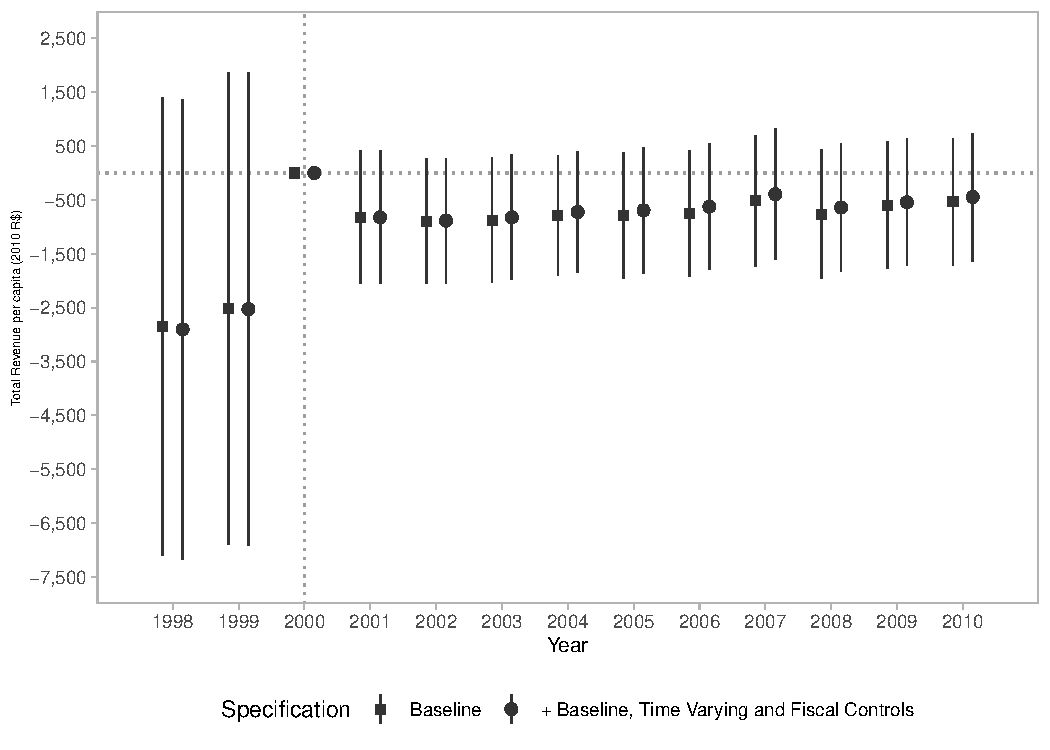
\includegraphics[width=\textwidth]{plots/finbra_reccorr_pcapita_dist_ec29_baseline_dist_ec29_baseline_6.pdf}
    \end{subfigure}
    \begin{subfigure}{0.49\textwidth}
        \centering
        \caption{\scriptsize Total Public Spending}\label{fig:6b}
        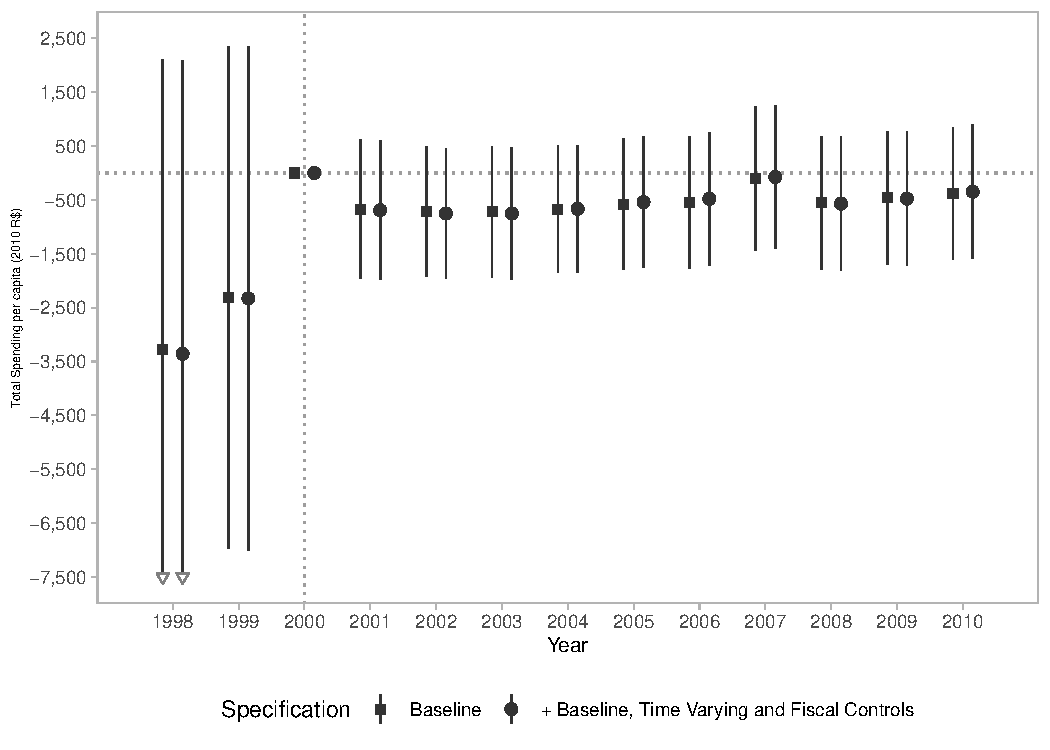
\includegraphics[width=\textwidth]{plots/finbra_desp_o_pcapita_dist_ec29_baseline_dist_ec29_baseline_6.pdf}
    \end{subfigure}
    
    \end{center}
    \scriptsize{Notes: The number of observations is 64224. DiD Estimates from Equation \ref{eq:2}. Independent variable is the distance to the EC/29 target in p.p. Square dots represent the baseline model with municipality and state-year fixed effects. Round dots represent fully saturated specification (Column 4 in regression Tables). Lines represent 95\% confidence intervals. Arrows, when present, indicate confidence intervals out of the plot bounds. Standard errors are clustered in the municipality level.}
    
\end{figure}

Panel C in Table \ref{table:fiscal} presents the results for total health spending, health spending by source and health spending by type. Our estimations suggests an effect of R\$ 530 for total Health Spending per capita, which is equivalent to a 27\% increase in spending relative to the baseline for our representative municipality, almost twice the effect on Health and Sanitation per capita. Additionally, this effect comes almost entirely from increases in spending from own resources, a 50\% increase relative to own resource spending in the baseline. We also find some substitution effects, with municipalities reducing some of its spending from intergovernmental transfers in health. All types of health spending were responsible for this increase in total health spending, but the increase in investment is the noteworthy, specially in relative terms. This estimate is associated with a 90\% increase in health investments. Baseline statistics show very little resources allocated in investments within total public health spending, the great majority of resources were allocated in human resources and in other administrative expenses. Considering the importance of capital investments to the supply of medical resources and the quality of medical services, and the little amount of investments in the baseline, an effect of this size is really relevant. Other expenditures, that includes mainly administrative spending, presents the strongest effect in per capita terms, almost half of the total increase in health spending per capita, equivalent to a 34\% increase relative to the baseline for the representative municipality. In opposition to the relevance investment in a health production function, administrative expenditure plays a much minor role in affecting health outcomes.

\begin{figure}[h!]
    \begin{center}
    \caption{Effects Public Spending per capita - By Type}\label{fig:7}
    \begin{subfigure}{0.32\textwidth}
        \centering
        \caption{\scriptsize Human Resources}\label{fig:7a}
        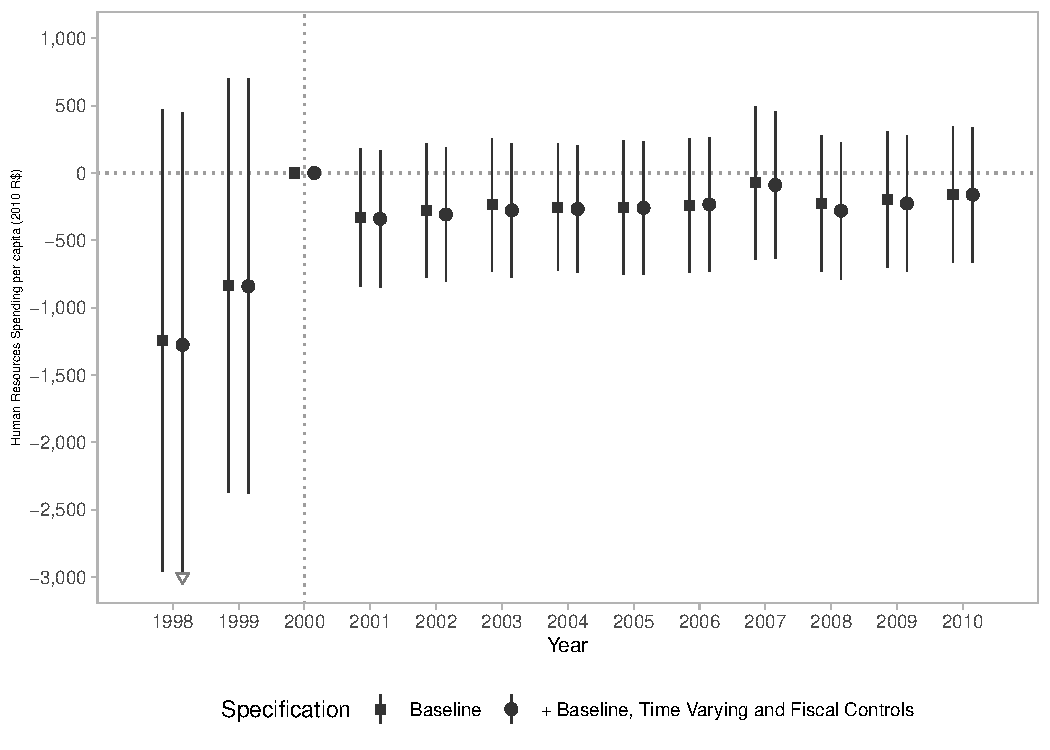
\includegraphics[width=\textwidth]{plots/finbra_desp_pessoal_pcapita_dist_ec29_baseline_dist_ec29_baseline_7.pdf}
    \end{subfigure}
    \begin{subfigure}{0.32\textwidth}
        \centering
        \caption{\scriptsize Investments}\label{fig:7b}
        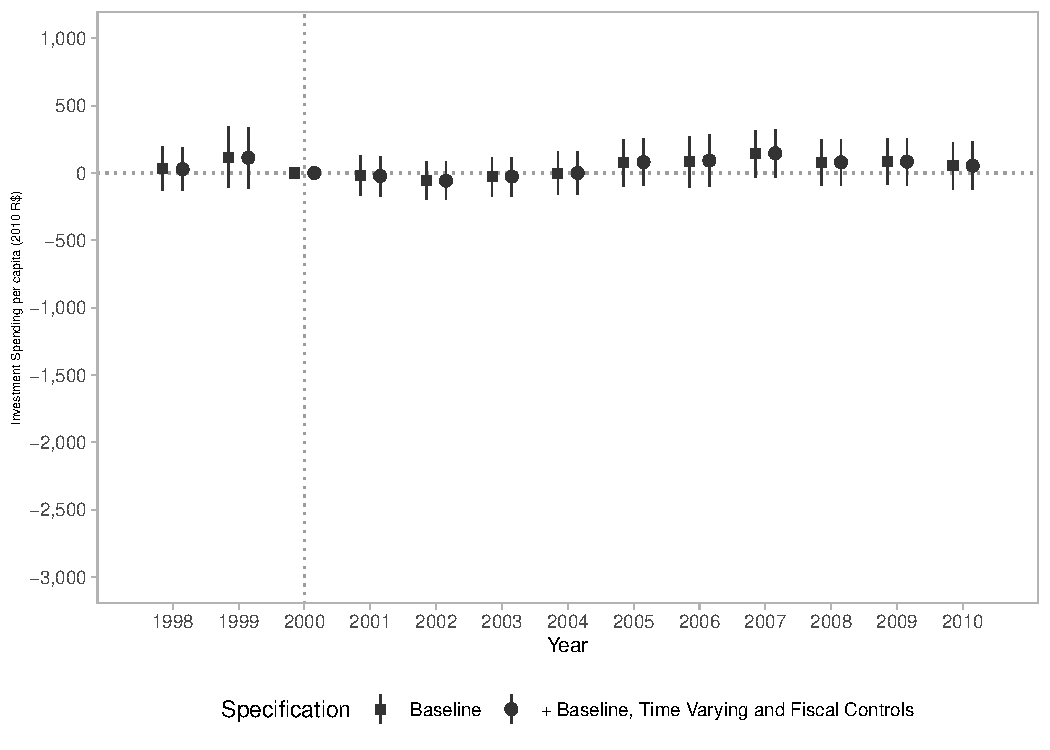
\includegraphics[width=\textwidth]{plots/finbra_desp_investimento_pcapita_dist_ec29_baseline_dist_ec29_baseline_7.pdf}
    \end{subfigure}
    \begin{subfigure}{0.32\textwidth}
        \centering
        \caption{\scriptsize Other}\label{fig:7c}
        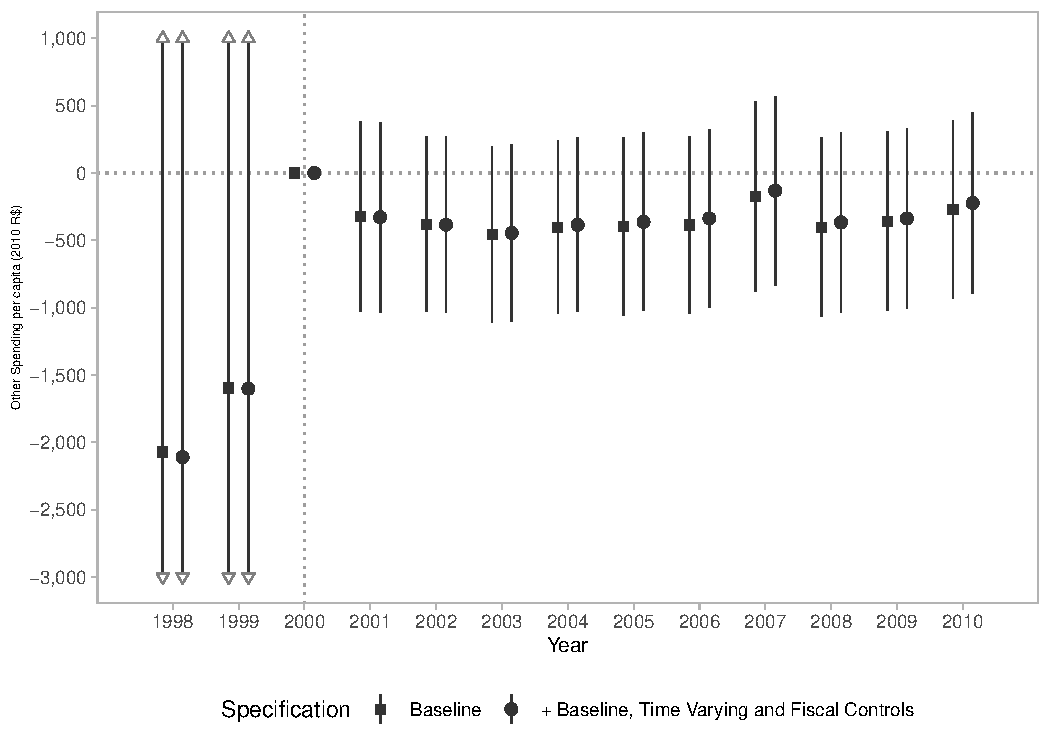
\includegraphics[width=\textwidth]{plots/finbra_desp_outros_nature_pcapita_dist_ec29_baseline_dist_ec29_baseline_7.pdf}
    \end{subfigure}
    
    \end{center}
    \scriptsize{Notes: The number of observations is 64224. DiD Estimates from Equation \ref{eq:2}. Independent variable is the distance to the EC/29 target in p.p. Square dots represent the baseline model with municipality and state-year fixed effects. Round dots represent fully saturated specification (Column 4 in regression Tables). Lines represent 95\% confidence intervals. Arrows, when present, indicate confidence intervals out of the plot bounds. Standard errors are clustered in the municipality level.}
    
\end{figure}

The clear pattern of increases in health and sanitation spending depicted in Figure \ref{fig:6a} can also be seen for SIOPS total health spending in Figure \ref{fig:6b}, but at different levels. Figure \ref{fig:7} suggests that this pattern is mostly influenced by dynamic of the effects on human resources spending (Figure \ref{fig:7a}). Investments, 3rd parties and other expenditures present a sharp increase in spending in the first one or two years after the EC/29 an than stabilize.


\subsection{Effects on Health Inputs}

In this subsection we aim to explore the pathways that mediate the relationship between health spending and health outcomes. For that, we explore the impacts of the EC/29 on several health inputs: primary care coverage, human resources, hospital infrastructure, primary care related infrastructure, ambulatorial production, and access to health services. 

\begin{table}[H]
\begin{footnotesize}
\begin{center}
\scalebox{0.65}{
\begin{threeparttable}[b]

  \centering
  \caption{Primary Care Coverage, Health Infrastructure and Human Resources}
     \begin{tabular}{rrcccr}
          &       &       &       &       &  \\
    \midrule
    \midrule
          &       & \multicolumn{4}{c}{Distance to EC9 target} \\
\cmidrule{3-6}          &       & (1)   & (2)   & (3)   & \multicolumn{1}{c}{(4)} \\
    \midrule
    \multicolumn{1}{p{23.645em}}{\textbf{A. Primary Care Coverage -  Extensive Margin}} &       &       &       &       &  \\
    \multicolumn{1}{l}{\multirow{2}[0]{*}{Population covered (share) by Community Health Agents}} &       & 0.25*** & 0.245*** & 0.245*** & \multicolumn{1}{c}{0.245***} \\
          &       & (0.056) & (0.055) & (0.055) & \multicolumn{1}{c}{(0.055)} \\
    \multicolumn{1}{l}{\multirow{2}[0]{*}{Population covered (share) by Family Health Agents}} &       & 0.187*** & 0.197*** & 0.201*** & \multicolumn{1}{c}{0.2***} \\
          &       & (0.059) & (0.058) & (0.058) & \multicolumn{1}{c}{(0.058)} \\
          &       &       &       &       &  \\
    \midrule
    \multicolumn{1}{p{23.645em}}{\textbf{B. Primary Care Coverage -  Intensive Margin}} &       &       &       &       &  \\
    \multicolumn{1}{l}{\multirow{2}[0]{*}{N. of People Visited by Primary Care Agents (per capita)}} &       & 0.294*** & 0.287*** & 0.298*** & \multicolumn{1}{c}{0.297***} \\
          &       & (0.101) & (0.097) & (0.097) & \multicolumn{1}{c}{(0.097)} \\
    \multicolumn{1}{l}{\multirow{2}[0]{*}{N. of People Visited by Community Health Agents (per capita)}} &       & -0.028 & -0.025 & -0.026 & \multicolumn{1}{c}{-0.026} \\
          &       & (0.053) & (0.053) & (0.053) & \multicolumn{1}{c}{(0.053)} \\
    \multicolumn{1}{l}{\multirow{2}[0]{*}{N. of People Visited by Family Health Agents (per capita)}} &       & 0.321*** & 0.311*** & 0.323*** & \multicolumn{1}{c}{0.322***} \\
          &       & (0.098) & (0.093) & (0.093) & \multicolumn{1}{c}{(0.093)} \\
    \multicolumn{1}{l}{\multirow{2}[0]{*}{N. of Household Visits (per capita)}} &       & 1.059*** & 1.057*** & 1.085*** & \multicolumn{1}{c}{1.085***} \\
          &       & (0.325) & (0.325) & (0.324) & \multicolumn{1}{c}{(0.324)} \\
    \multicolumn{1}{l}{\multirow{2}[0]{*}{N. of Household Visits by Community Health Agents (per capita)}} &       & 0.396 & 0.375 & 0.368 & \multicolumn{1}{c}{0.37} \\
          &       & (0.277) & (0.279) & (0.279) & \multicolumn{1}{c}{(0.278)} \\
    \multicolumn{1}{l}{\multirow{2}[0]{*}{N. of Household Visits by Family Health Agents (per capita)}} &       & 0.653** & 0.676*** & 0.711*** & \multicolumn{1}{c}{0.71***} \\
          &       & (0.256) & (0.247) & (0.246) & \multicolumn{1}{c}{(0.246)} \\
    \multicolumn{1}{l}{\multirow{2}[0]{*}{N. of Appointments (per capita)}} &       & 0.181* & 0.181* & 0.186* & \multicolumn{1}{c}{0.187*} \\
          &       & (0.108) & (0.108) & (0.109) & \multicolumn{1}{c}{(0.109)} \\
    \multicolumn{1}{l}{\multirow{2}[0]{*}{N. of Appointments from Community Health Program (per capita)}} &       & -0.015 & -0.013 & -0.013 & \multicolumn{1}{c}{-0.013} \\
          &       & (0.02) & (0.021) & (0.021) & \multicolumn{1}{c}{(0.021)} \\
    \multicolumn{1}{l}{\multirow{2}[0]{*}{N. of Appointments from Family Health Program (per capita)}} &       & 0.192* & 0.188* & 0.193* & \multicolumn{1}{c}{0.194*} \\
          &       & (0.108) & (0.107) & (0.108) & \multicolumn{1}{c}{(0.108)} \\
          &       &       &       &       &  \\
    \midrule
    \multicolumn{1}{p{23.645em}}{\textbf{C. Number of Health Facilities (per capita * 1000) with}} &       &       &       &       &  \\
    \multicolumn{1}{l}{\multirow{2}[0]{*}{Ambulatory Service}} &       & -0.094** & -0.085** & -0.08* & \multicolumn{1}{c}{ -0.08* } \\
          &       & (0.042) & (0.043) & (0.042) & \multicolumn{1}{c}{ (0.042) } \\
    \multicolumn{1}{l}{\multirow{2}[0]{*}{Ambulatory Service and PSF Teams}} &       & 0.061** & 0.059** & 0.063** & \multicolumn{1}{c}{ 0.063** } \\
          &       & (0.029) & (0.028) & (0.028) & \multicolumn{1}{c}{ (0.028) } \\
    \multicolumn{1}{l}{\multirow{2}[0]{*}{Ambulatory Service and ACS Teams}} &       & 0.046 & 0.052 & 0.056* & \multicolumn{1}{c}{ 0.056* } \\
          &       & (0.033) & (0.032) & (0.032) & \multicolumn{1}{c}{ (0.032) } \\
    \multicolumn{1}{l}{\multirow{2}[0]{*}{Ambulatory Service and Community Doctors}} &       & 0.054* & 0.056* & 0.061** & \multicolumn{1}{c}{ 0.061** } \\
          &       & (0.032) & (0.031) & (0.031) & \multicolumn{1}{c}{ (0.031) } \\
    \multicolumn{1}{l}{\multirow{2}[0]{*}{Ambulatory Service and PSF Doctors}} &       & 0.047 & 0.051* & 0.056* & \multicolumn{1}{c}{ 0.056* } \\
          &       & (0.032) & (0.03) & (0.03) & \multicolumn{1}{c}{ (0.03) } \\
    \multicolumn{1}{l}{\multirow{2}[0]{*}{Ambulatory Service and PSF Nurses}} &       & 0.033* & 0.032 & 0.034* & \multicolumn{1}{c}{ 0.034* } \\
          &       & (0.02) & (0.02) & (0.02) & \multicolumn{1}{c}{ (0.02) } \\
    \multicolumn{1}{l}{\multirow{2}[0]{*}{Ambulatory Service and PSF Nursing Assistants}} &       & 0.061** & 0.066** & 0.07** & \multicolumn{1}{c}{ 0.07** } \\
          &       & (0.031) & (0.03) & (0.029) & \multicolumn{1}{c}{ (0.029) } \\
    \multicolumn{1}{l}{\multirow{2}[0]{*}{Ambulatory Service and ACS Nurses}} &       & 0.02  & 0.023 & 0.028 & \multicolumn{1}{c}{ 0.028 } \\
          &       & (0.03) & (0.029) & (0.029) & \multicolumn{1}{c}{ (0.029) } \\
          &       &       &       &       &  \\
    \midrule
    \multicolumn{1}{p{23.645em}}{\textbf{D. Hospital and Beds}} &       &       &       &       &  \\
    \multicolumn{1}{l}{\multirow{2}[0]{*}{N. of Hospital Beds (per capita * 1000)}} &       & -0.933** & -0.803** & -0.779** & \multicolumn{1}{c}{ -0.78** } \\
          &       & (0.373) & (0.373) & (0.372) & \multicolumn{1}{c}{ (0.372) } \\
    \multicolumn{1}{l}{\multirow{2}[0]{*}{Presence of Hospital}} &       & -0.11*** & -0.082** & -0.082** & \multicolumn{1}{c}{ -0.082** } \\
          &       & (0.041) & (0.039) & (0.039) & \multicolumn{1}{c}{ (0.039) } \\
          &       &       &       &       &  \\
    \midrule
    \midrule
          &       &       &       &       &  \\
    \end{tabular}%
    
    
  \label{table:infra}%

\end{threeparttable}
}
\end{center}
\end{footnotesize}
\end{table}

First we analyse the effects on primary care coverage at the extensive and intensive margin (Table \ref{table:infra}, Panel A and B). We find significant effects on the share of population covered by the Community Health program and by Family Health Program. Though significant and positive, these effects are quite small. The representative municipality only increased by 2 percentage points the share of the population covered by these primary care programs. On the other hand, the effects on the intensive margin are much more pronounced and our estimates suggests that they come mainly from the Family Health Program. We find significant increases in the number of people visited and in the number of household visits and appointments by Family Health Agents. They are equivalent to a 21\% and 11\% increase relative to the baseline, respectively, for our representative municipality. Figure \ref{fig:8} shows the dynamic effects for the extensive margin and Figure \ref{fig:9} the dynamic effects for the intensive margin of primary care coverage. The temporal patterns of this effects resemble the pattern in health spending increase, where the effect is increasing in the first years after the EC/29 and becomes steady after 2004. 

\begin{figure}[h!]
    \begin{center}
    \caption{Effects on Public Spending per capita - By Category}\label{fig:8}
    \begin{subfigure}{0.48\textwidth}
        \caption{\scriptsize Health and Sanitation}\label{fig:8a}
        \centering
        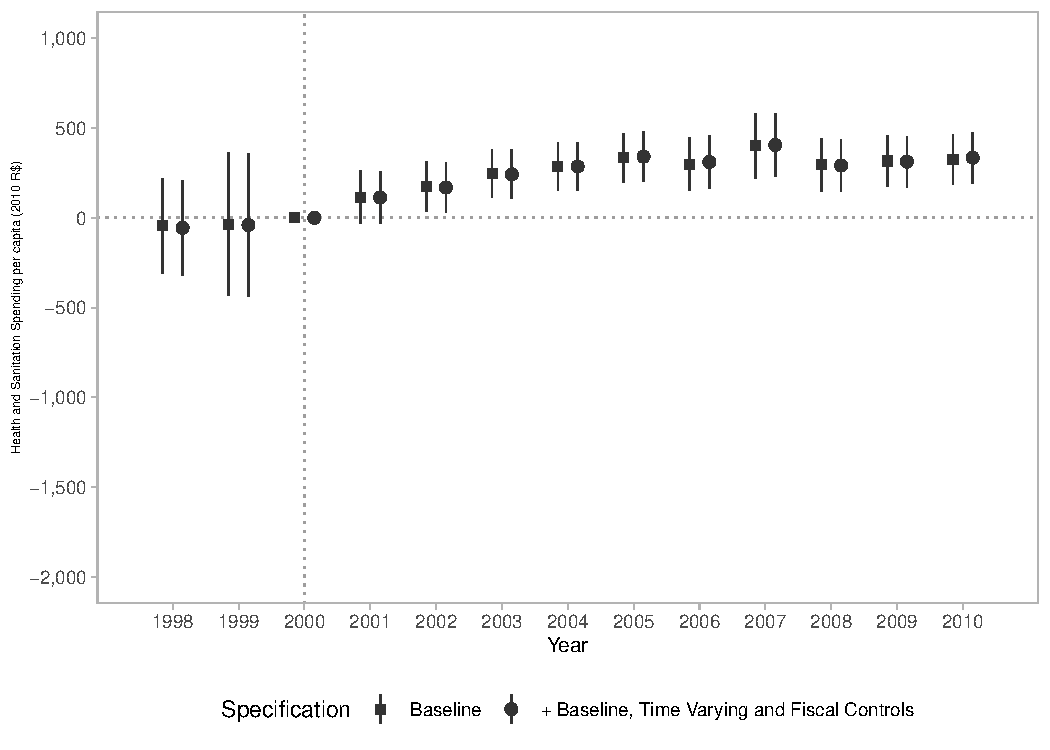
\includegraphics[width=\textwidth]{plots/finbra_desp_saude_san_pcapita_dist_ec29_baseline_dist_ec29_baseline_8.pdf}
    \end{subfigure}
    \begin{subfigure}{0.48\textwidth}
        \centering
        \caption{\scriptsize Education and Culture}\label{fig:8b}
        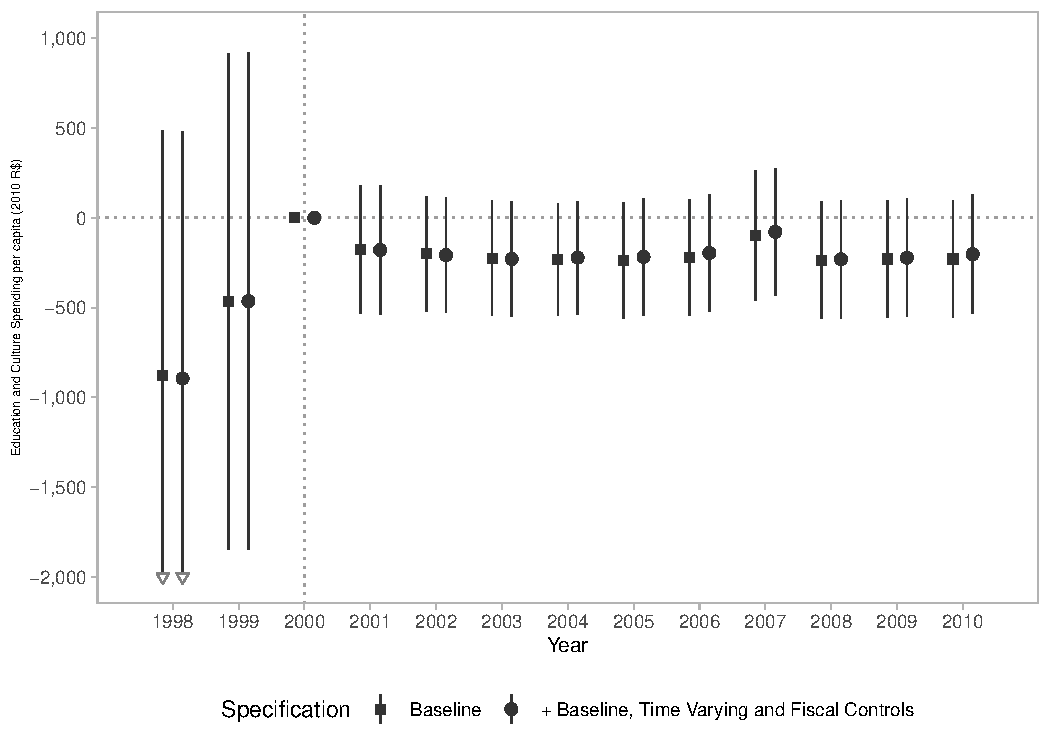
\includegraphics[width=\textwidth]{plots/finbra_desp_educ_cultura_pcapita_dist_ec29_baseline_dist_ec29_baseline_8.pdf}
    \end{subfigure}
    \begin{subfigure}{0.48\textwidth}
        \centering
        \caption{\scriptsize Social Assistance}\label{fig:8c}
        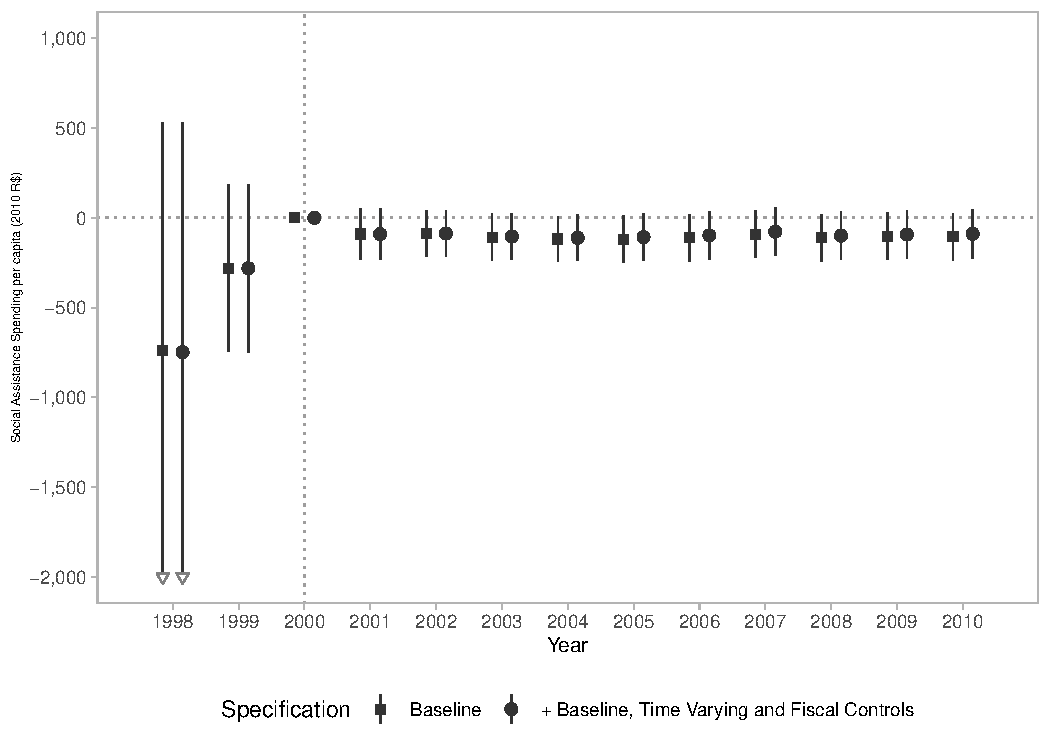
\includegraphics[width=\textwidth]{plots/finbra_desp_assist_prev_pcapita_dist_ec29_baseline_dist_ec29_baseline_8.pdf}
    \end{subfigure}
    \begin{subfigure}{0.48\textwidth}
        \centering
        \caption{\scriptsize Transport}\label{fig:8d}
        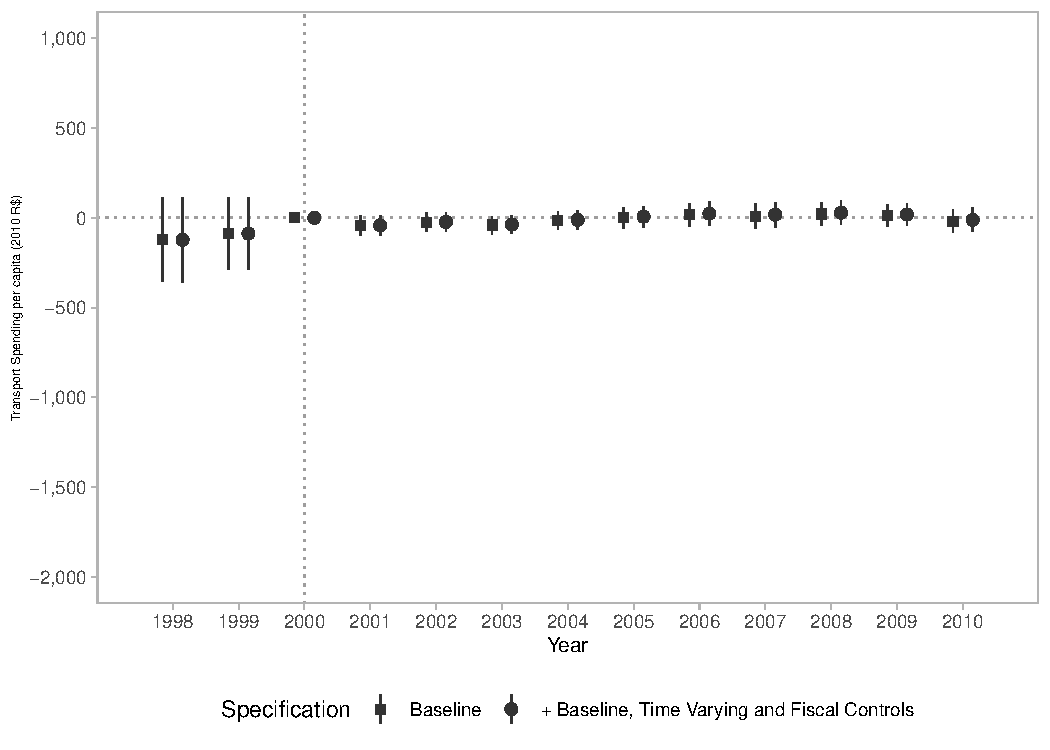
\includegraphics[width=\textwidth]{plots/finbra_desp_transporte_pcapita_dist_ec29_baseline_dist_ec29_baseline_8.pdf}
    \end{subfigure}
    \begin{subfigure}{0.48\textwidth}
        \centering
        \caption{\scriptsize Housing and Urban}\label{fig:8e}
        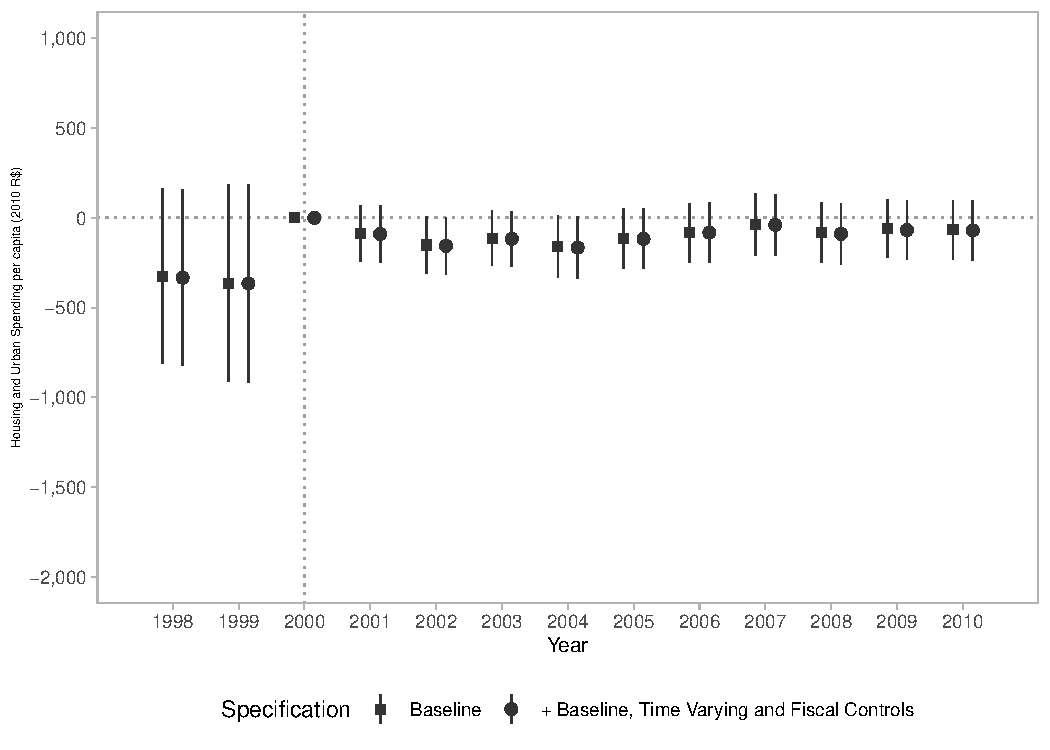
\includegraphics[width=\textwidth]{plots/finbra_desp_hab_urb_pcapita_dist_ec29_baseline_dist_ec29_baseline_8.pdf}
    \end{subfigure}
    \begin{subfigure}{0.48\textwidth}
        \centering
        \caption{\scriptsize Spending in Other Categories}\label{fig:8f}
        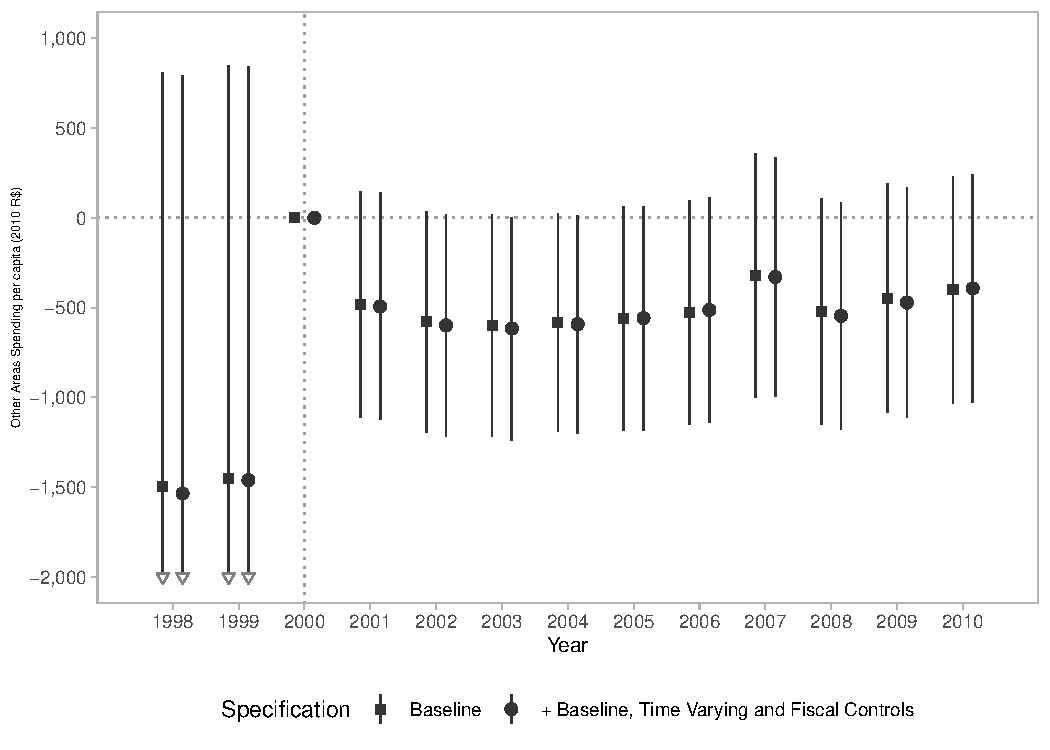
\includegraphics[width=\textwidth]{plots/finbra_desp_outros_area_pcapita_dist_ec29_baseline_dist_ec29_baseline_8.pdf}
    \end{subfigure}
    
    \end{center}
    \scriptsize{Notes: The number of observations is 64224. DiD Estimates from Equation \ref{eq:2}. Independent variable is the distance to the EC/29 target in p.p. Square dots represent the baseline model with municipality and state-year fixed effects. Round dots represent fully saturated specification (Column 4 in regression Tables). Lines represent 95\% confidence intervals. Arrows, when present, indicate confidence intervals out of the plot bounds. Standard errors are clustered in the municipality level.}
    
\end{figure}

\begin{figure}[h!]
    \begin{center}
    \caption{Effects on Public Health Spending per capita}\label{fig:9}
    \begin{subfigure}{0.48\textwidth}
        \caption{\scriptsize Health and Sanitation (Finbra)}\label{fig:9a}
        \centering
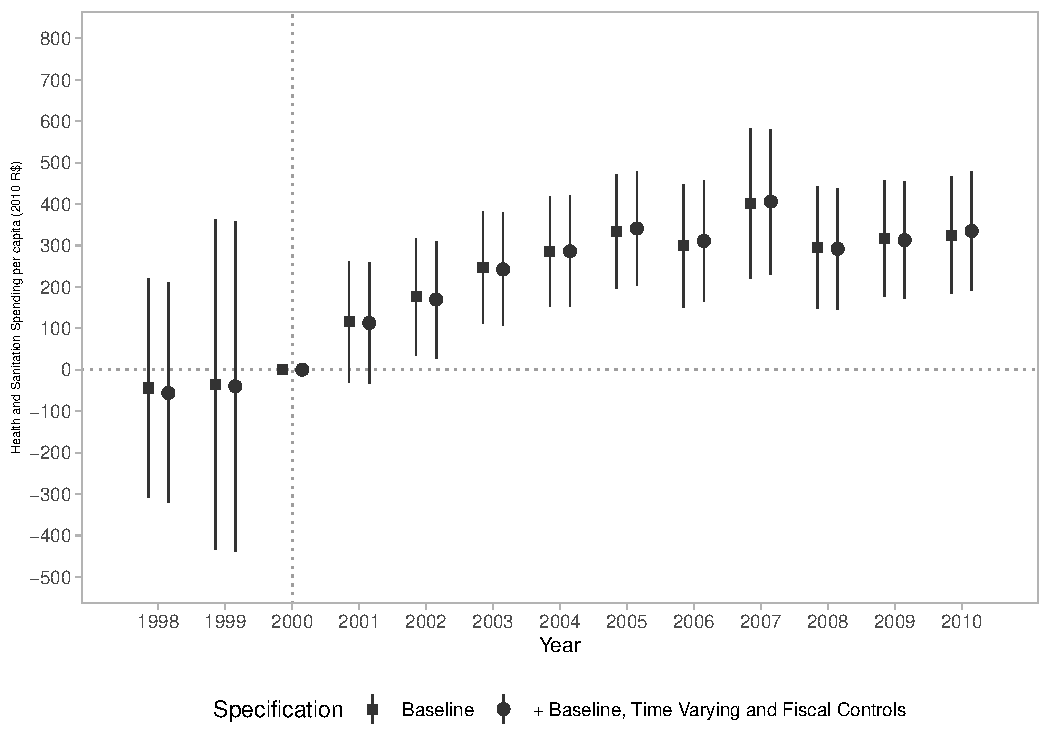
\includegraphics[width=\textwidth]{plots/finbra_desp_saude_san_pcapita_dist_ec29_baseline_dist_ec29_baseline_9.pdf}
    \end{subfigure}
    \begin{subfigure}{0.48\textwidth}
        \centering
        \caption{\scriptsize Total Health Spending (SIOPS)}\label{fig:9b}
        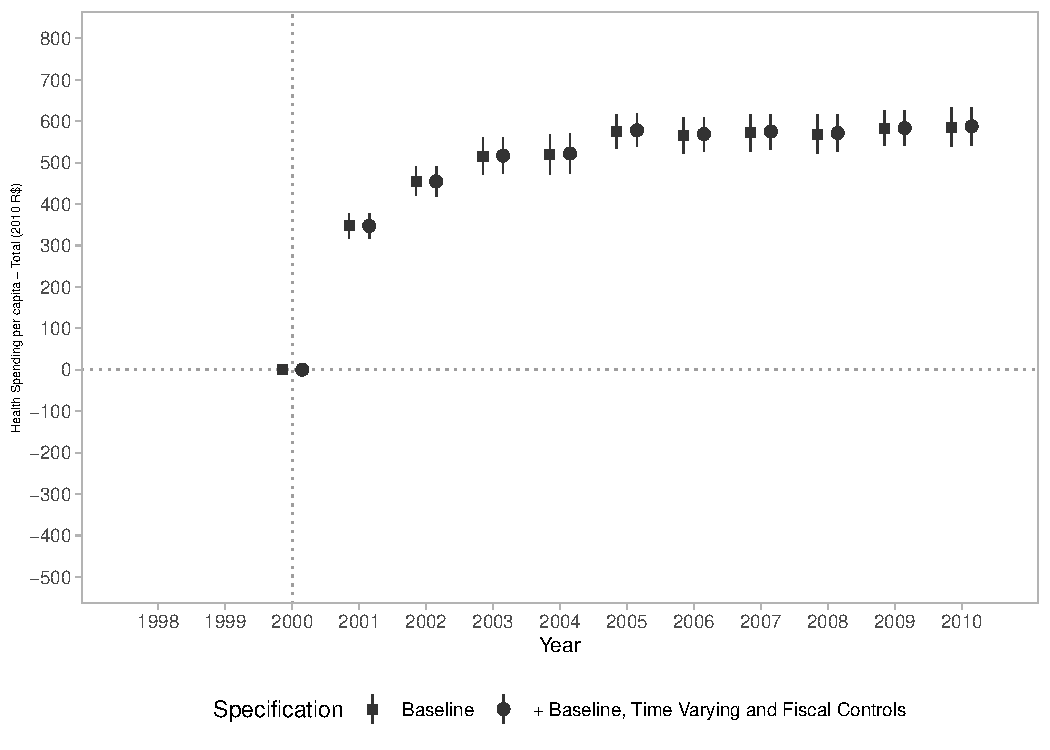
\includegraphics[width=\textwidth]{plots/siops_despsaude_pcapita_dist_ec29_baseline_dist_ec29_baseline_9.pdf}
    \end{subfigure}
    \begin{subfigure}{0.48\textwidth}
        \centering
        \caption{\scriptsize Health Spending - Own Resources (SIOPS)}\label{fig:9c}
        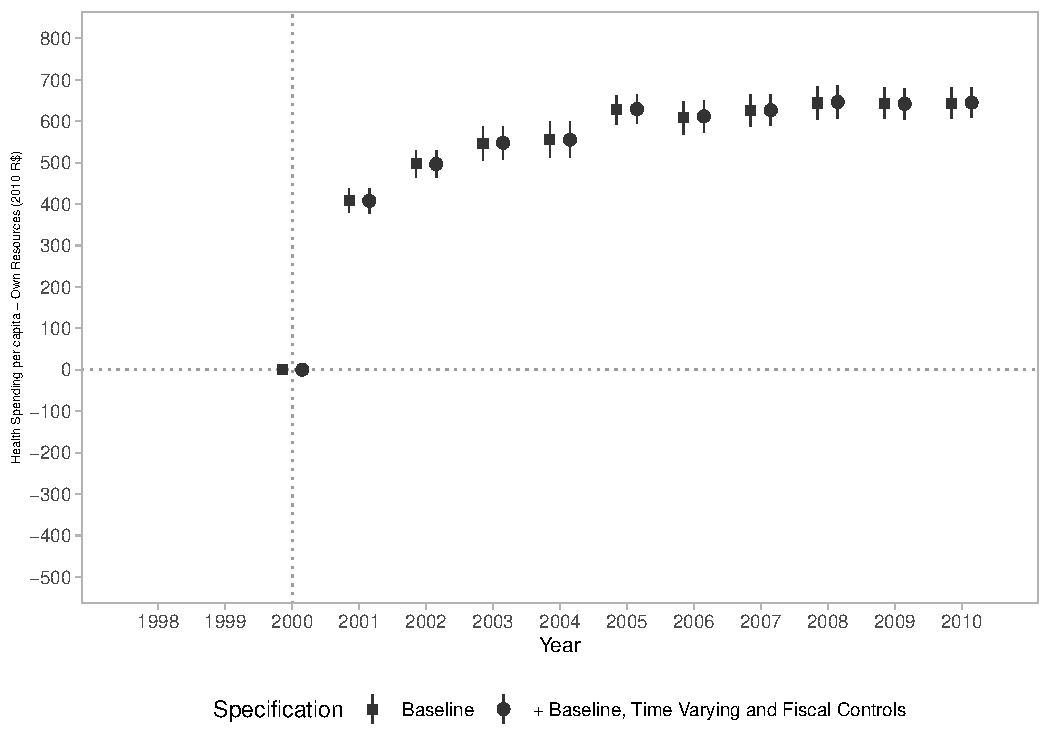
\includegraphics[width=\textwidth]{plots/siops_desprecpropriosaude_pcapita_dist_ec29_baseline_dist_ec29_baseline_9.pdf}
    \end{subfigure}
    \begin{subfigure}{0.48\textwidth}
        \centering
        \caption{\scriptsize Health Spending  - Transfers (SIOPS)}\label{fig:9d}
        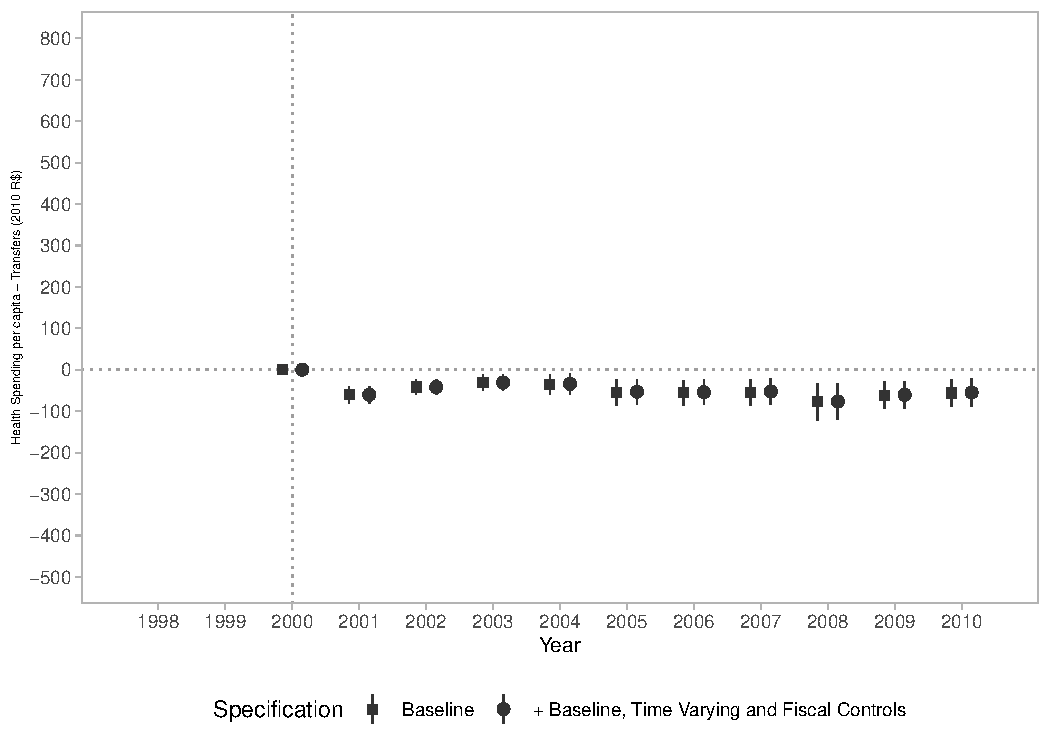
\includegraphics[width=\textwidth]{plots/siops_despexrecproprio_pcapita_dist_ec29_baseline_dist_ec29_baseline_9.pdf}
    \end{subfigure}
    
    \end{center}
    
\end{figure}

Panel C presents our results on the public health sector human resources. We find no significant effect for the number of doctors and nurses, but Figures \ref{fig:10a} and \ref{fig:10b} suggests some effect taking place after 2005. On the other hand, we find significant effects in the number of nursing assistants and administrative professionals, a 13\% and 15\% increase, respectively, relative to the baseline. While Figure \ref{fig:10c} indicates a gradual effect trend after the EC/29, Figure \ref{fig:10d} suggests a sharp increase in the number of administrative personnel right after the EC/29. Not coincidentally, this pattern resembles the pattern found in other expenditures within health spending (Figure \ref{fig:7d}), that, as mentioned before, includes mainly administrative spending. 

\begin{figure}[h!]
    \begin{center}
    \caption{Effects on Public Health Spending per capita - By Type}\label{fig:10}
    \begin{subfigure}{0.48\textwidth}
        \centering
        \caption{\scriptsize Human Resources}\label{fig:10a}
        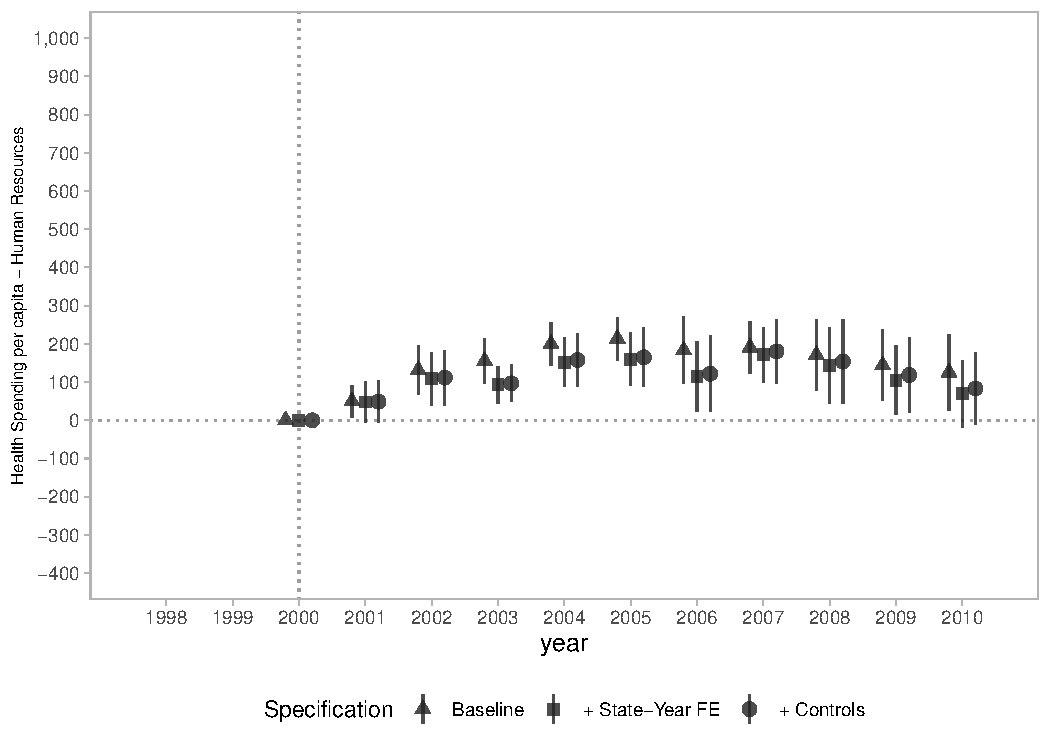
\includegraphics[width=\textwidth]{plots/spending/siops_desppessoal_pcapita_dist_ec29_baseline_dist_ec29_baseline_full.pdf}
    \end{subfigure}
    \begin{subfigure}{0.48\textwidth}
        \centering
        \caption{\scriptsize Investiment}\label{fig:10b}
        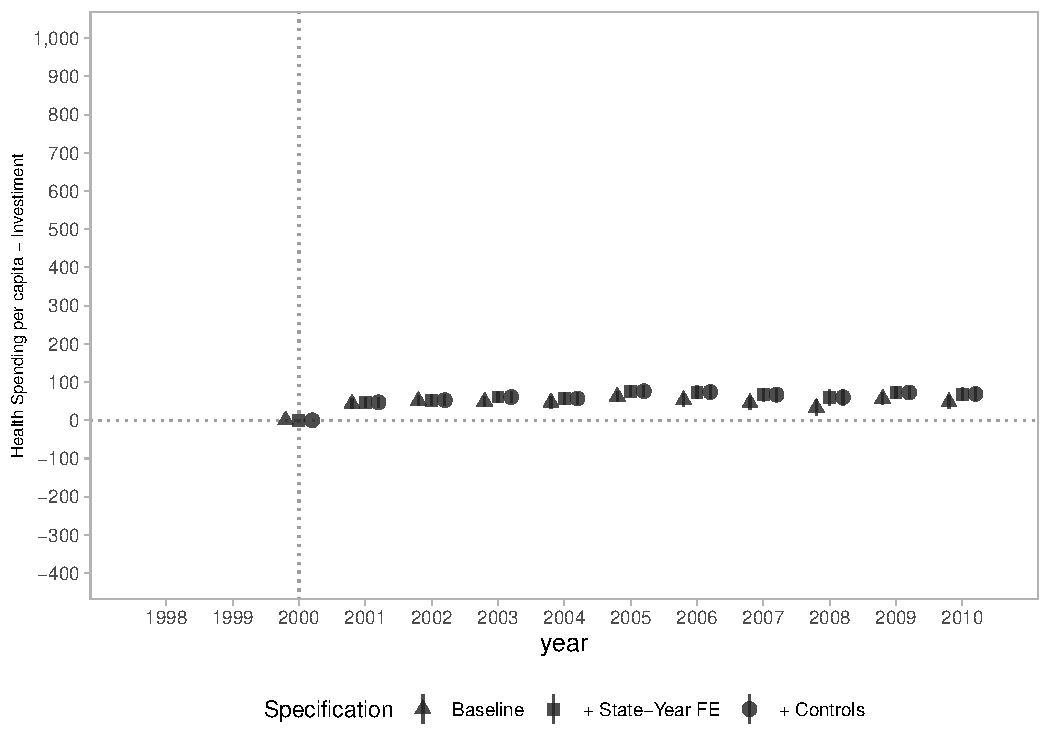
\includegraphics[width=\textwidth]{plots/spending/siops_despinvest_pcapita_dist_ec29_baseline_dist_ec29_baseline_full.pdf}
    \end{subfigure}
    \begin{subfigure}{0.48\textwidth}
        \centering
        \caption{\scriptsize 3rd parties services}\label{fig:10c}
        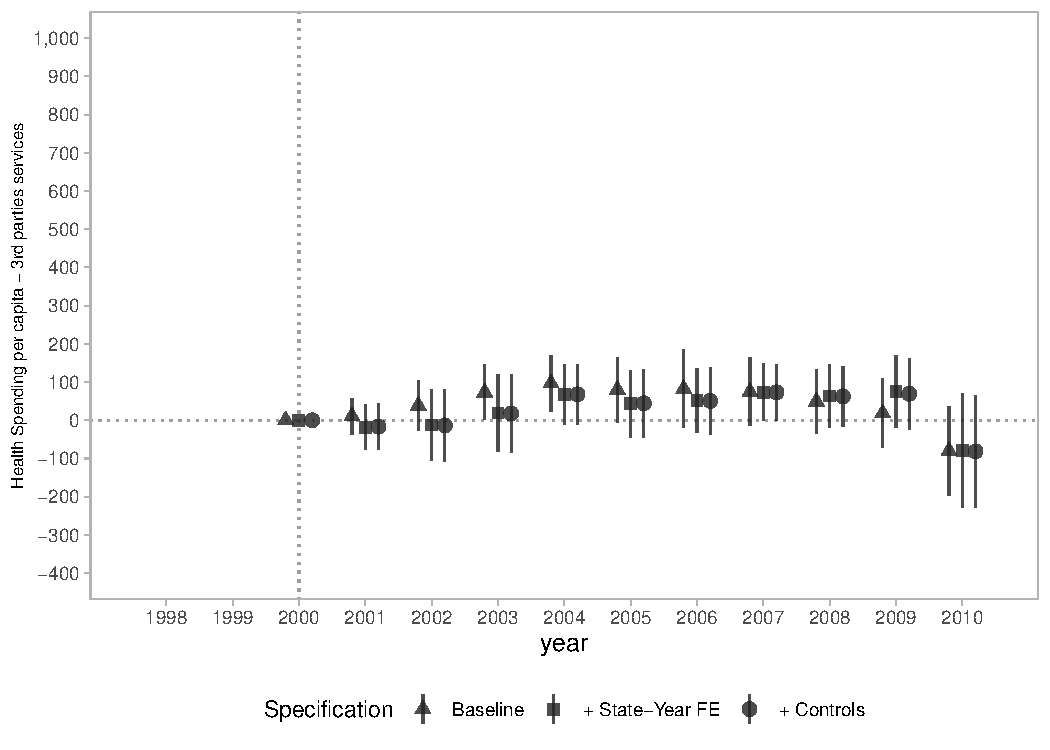
\includegraphics[width=\textwidth]{plots/spending/siops_despservicoster_pcapita_dist_ec29_baseline_dist_ec29_baseline_full.pdf}
    \end{subfigure}
    \begin{subfigure}{0.48\textwidth}
        \centering
        \caption{\scriptsize Other Expenditures}\label{fig:10d}
        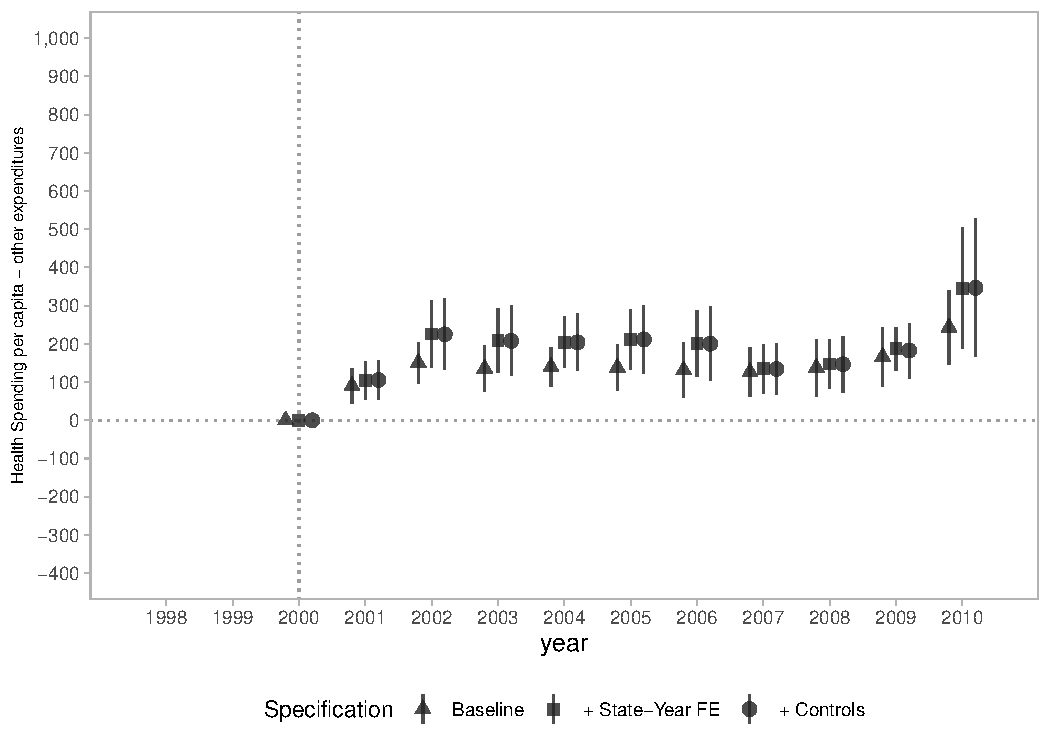
\includegraphics[width=\textwidth]{plots/spending/siops_despoutros_pcapita_dist_ec29_baseline_dist_ec29_baseline_full.pdf}
    \end{subfigure}
    
    \end{center}
    
\end{figure}

Next, panel D shows the results for health infrastructure. The number of municipal hospital per 1000 inhabitants presented a significant increase of 0.16. This effect represents a sizable variation of 27\% relative to the baseline number of hospitals for the representative municipality. Moreover, Figure \ref{fig:11a} suggests that the effect follows a similar dynamic pattern as the increase in investment spending within health (Figure \ref{fig:7b}). In this analysis we leverage the variation in municipal health spending induced by the EC/29 within state governments, so one would not expect to see increases in the number of hospital from other governmental spheres or from the private sector. Our results validates that. Yet, the point estimates for the number of Federal, State and Private hospitals are negative, which could suggest some substitution effects in the supply of hospitals. These results would be worrisome if the effects were large, as mortality outcomes can be affected by the supply of hospitals, but that is not what the point estimates and Figure \ref{fig:11b} \ref{fig:11b} suggests. Our results also indicate some marginally significant reduction in the number of health facilities with ambulatory service, but this effect is rather small, representing a reduction of 1.5\% relative to the baseline for the representative municipality.

\begin{figure}[h!]
    \begin{center}
    \caption{Effects on Primary Care Coverage - Extensive Margin}\label{fig:11}
    \begin{subfigure}{0.48\textwidth}
        \centering
        \caption{\scriptsize Population Covered by Community Health Agents}\label{fig:11a}
        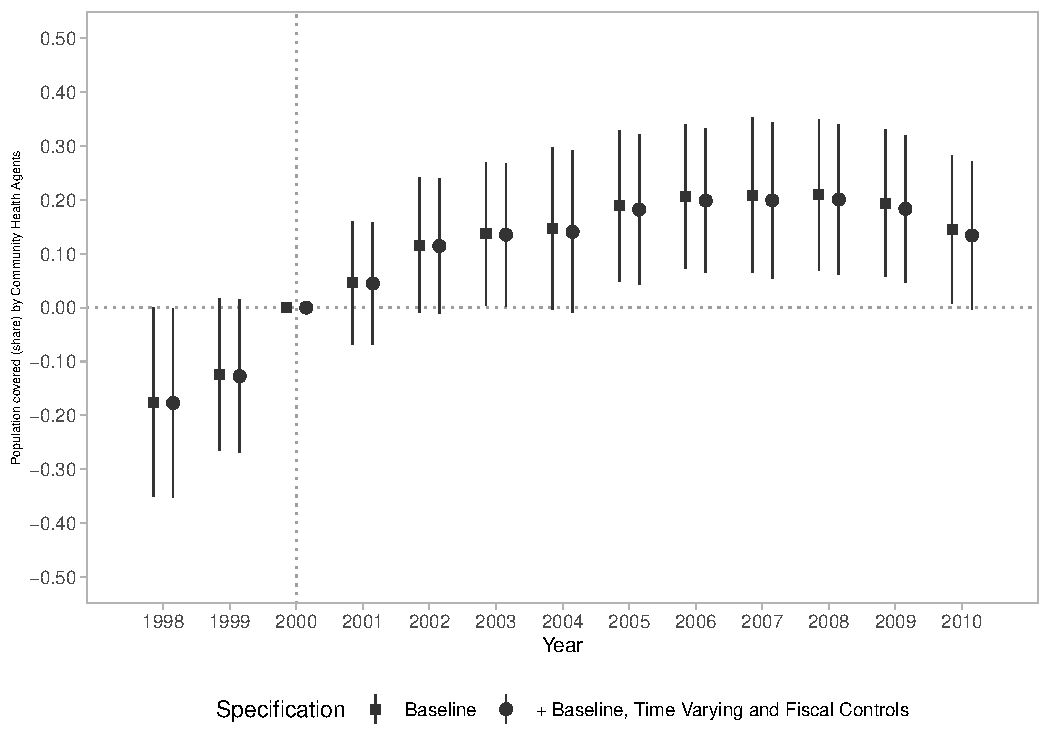
\includegraphics[width=\textwidth]{plots/ACS_popprop_dist_ec29_baseline_dist_ec29_baseline_11.pdf}
    \end{subfigure}
    \begin{subfigure}{0.48\textwidth}
        \centering
        \caption{\scriptsize Population Covered by Family Health Agents}\label{fig:1b}
        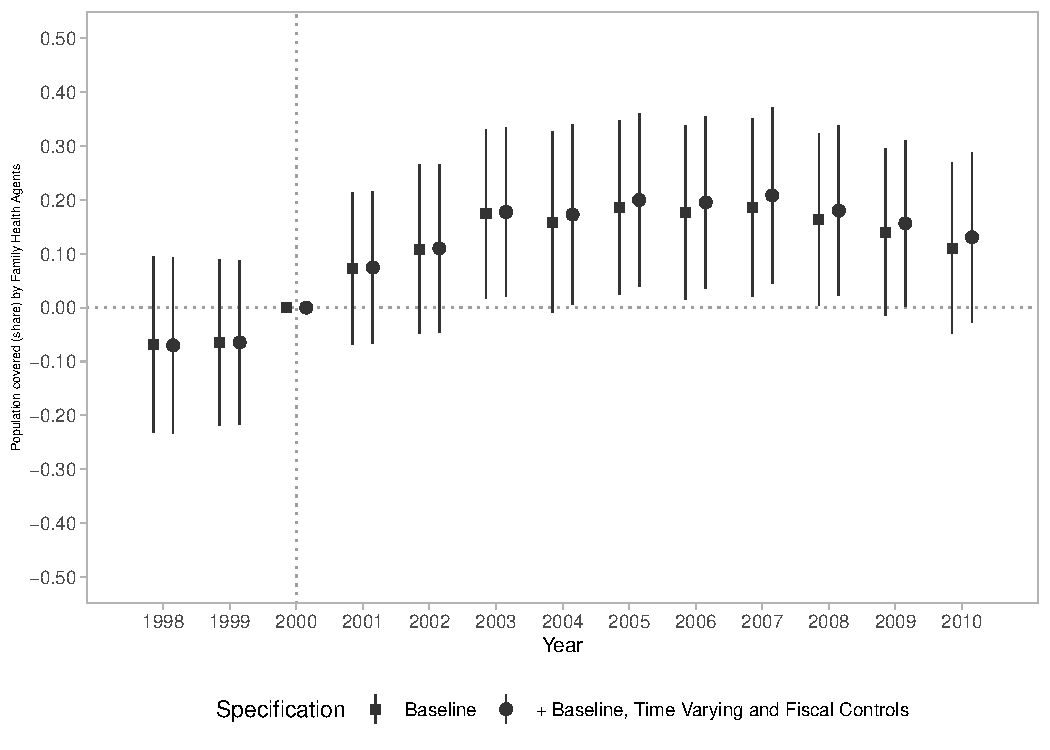
\includegraphics[width=\textwidth]{plots/eSF_popprop_dist_ec29_baseline_dist_ec29_baseline_11.pdf}
    \end{subfigure}
    
    \end{center}
    
\end{figure}

We also find significant effects on the number of health facilities with ambulatorial services and professionals related to primary care (Panel E of Table \ref{table:infra} and Figure \ref{fig:12}), with effects ranging from 5\% to 10\% relative to the baseline.

\begin{figure}[h!]
    \begin{center}
    \caption{Effects on Primary Care Coverage - Intensive Margin}\label{fig:12}
    \begin{subfigure}{0.32\textwidth}
        \caption{\scriptsize N. of People Visited}\label{fig:12a}
        \centering
        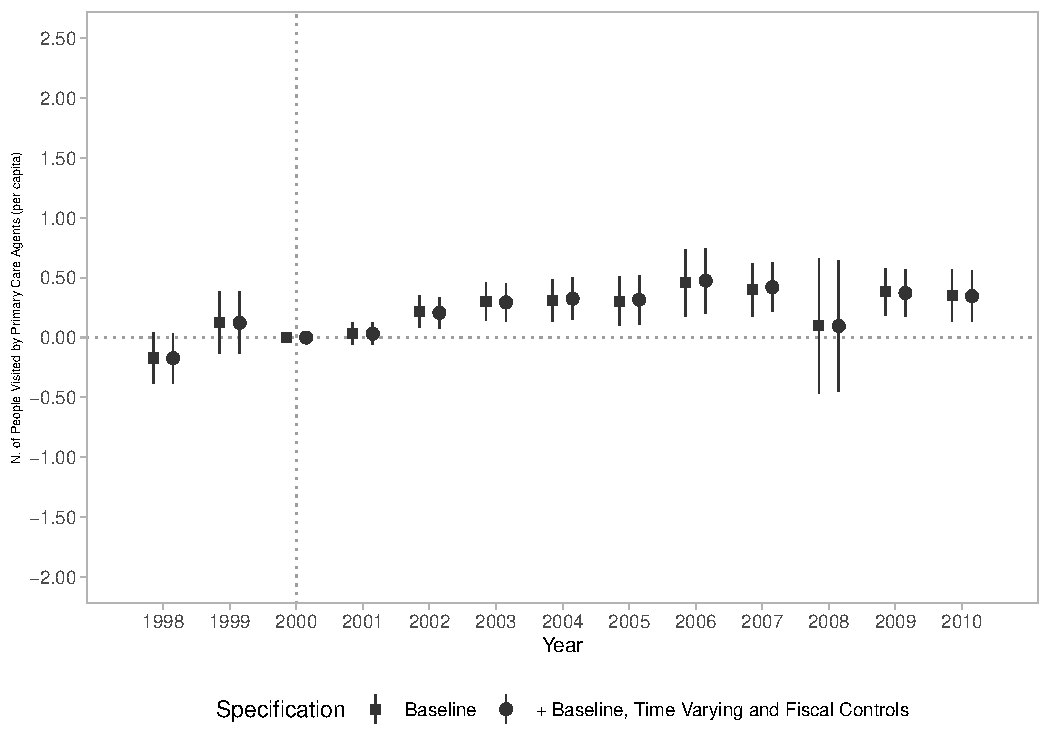
\includegraphics[width=\textwidth]{plots/siab_accomp_especif_pcapita_dist_ec29_baseline_dist_ec29_baseline_12.pdf}
    \end{subfigure}
    \begin{subfigure}{0.32\textwidth}
        \centering
        \caption{\scriptsize People Visited by CH Agents}\label{fig:12b}
        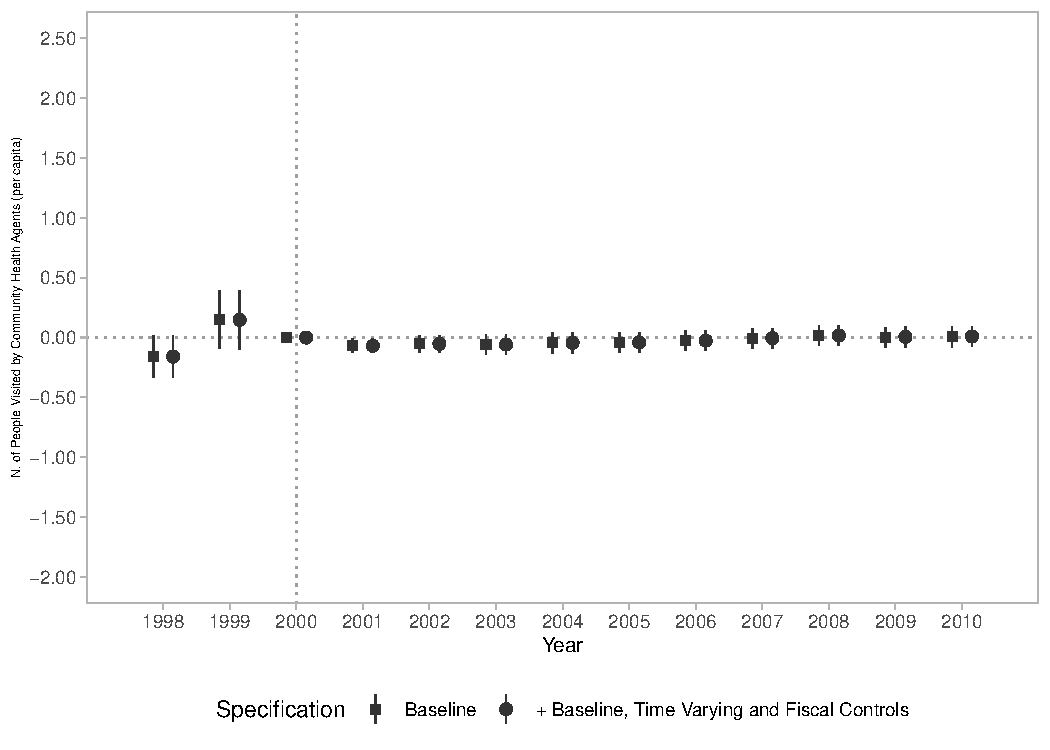
\includegraphics[width=\textwidth]{plots/siab_accomp_especif_pacs_pcapita_dist_ec29_baseline_dist_ec29_baseline_12.pdf}
    \end{subfigure}
    \begin{subfigure}{0.32\textwidth}
        \centering
        \caption{\scriptsize People Visited by FH Agents}\label{fig:12c}
        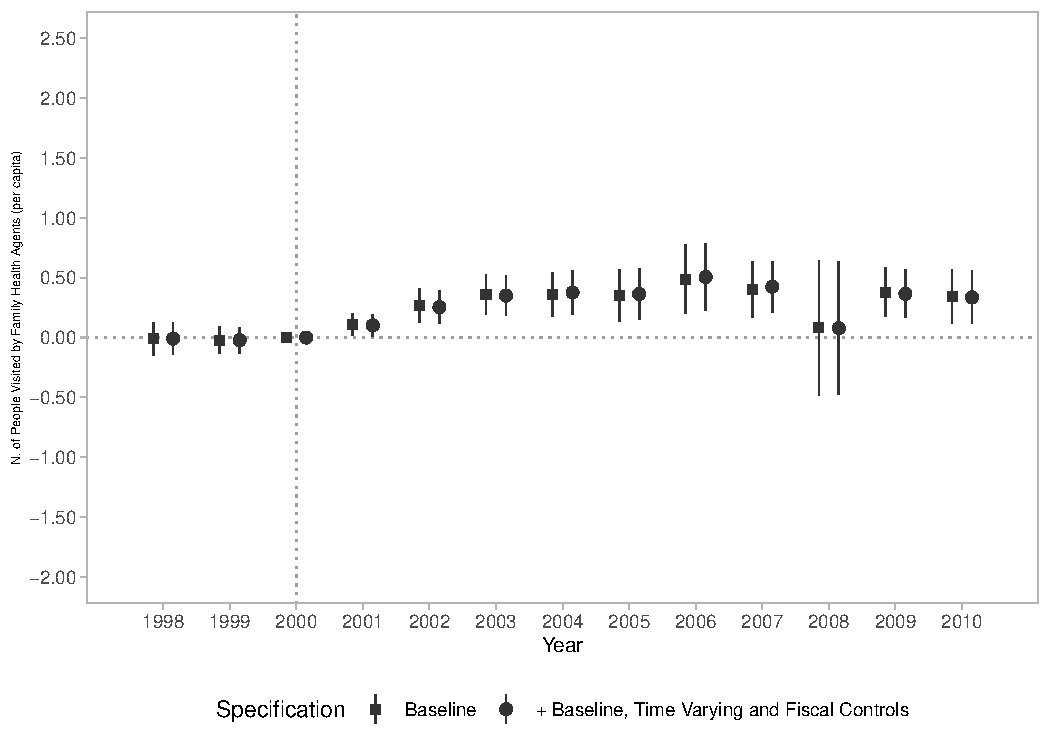
\includegraphics[width=\textwidth]{plots/siab_accomp_especif_psf_pcapita_dist_ec29_baseline_dist_ec29_baseline_12.pdf}
    \end{subfigure}
        \begin{subfigure}{0.32\textwidth}
        \caption{\scriptsize N. of Household Visits}\label{fig:12d}
        \centering
        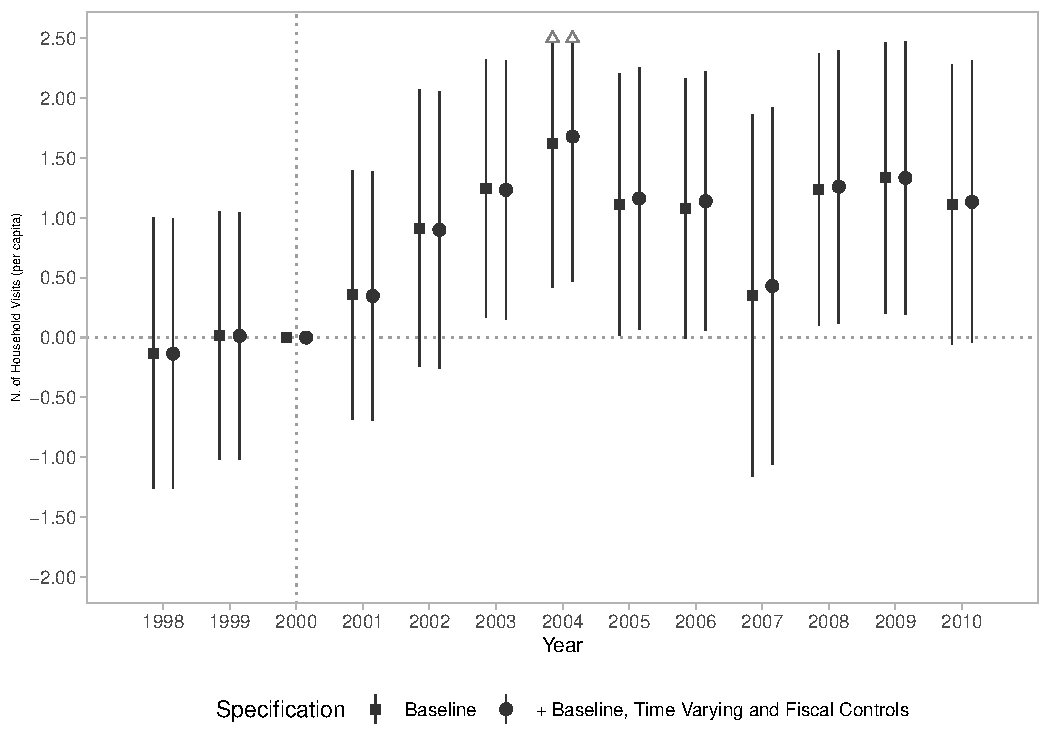
\includegraphics[width=\textwidth]{plots/siab_visit_cha_pcapita_dist_ec29_baseline_dist_ec29_baseline_12.pdf}
    \end{subfigure}
    \begin{subfigure}{0.32\textwidth}
        \centering
        \caption{\scriptsize N. of Household Visits by CH Agents}\label{fig:12e}
        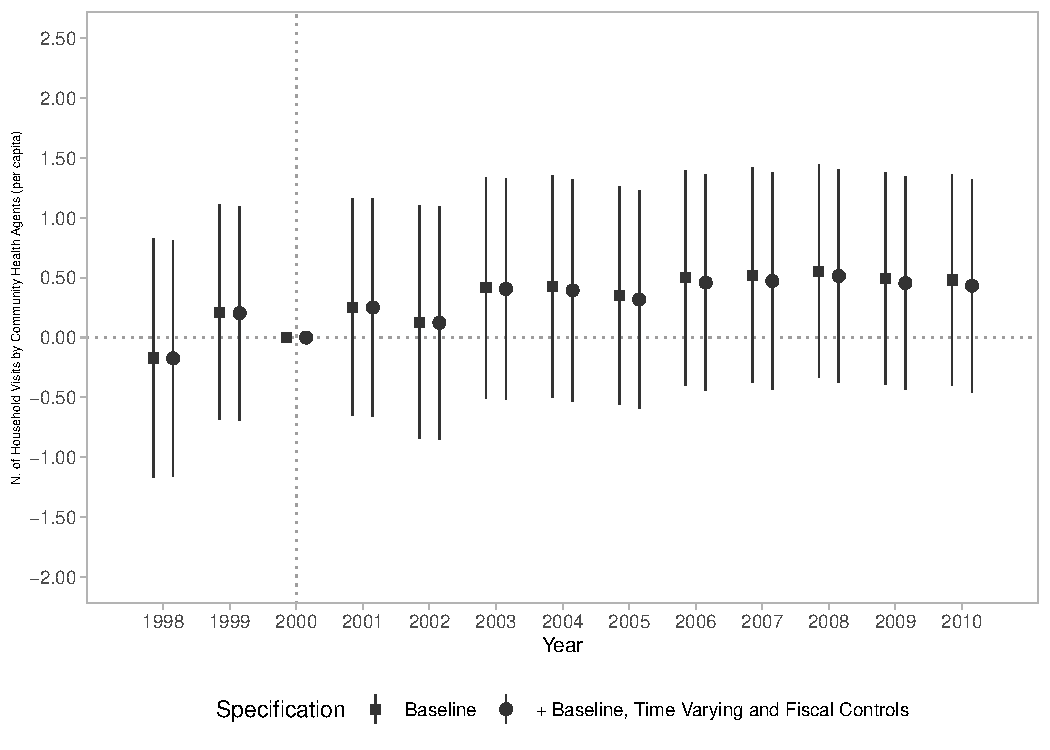
\includegraphics[width=\textwidth]{plots/siab_visit_cha_pacs_pcapita_dist_ec29_baseline_dist_ec29_baseline_12.pdf}
    \end{subfigure}
    \begin{subfigure}{0.32\textwidth}
        \centering
        \caption{\scriptsize N. of Household Visits by FH Agents}\label{fig:12f}
        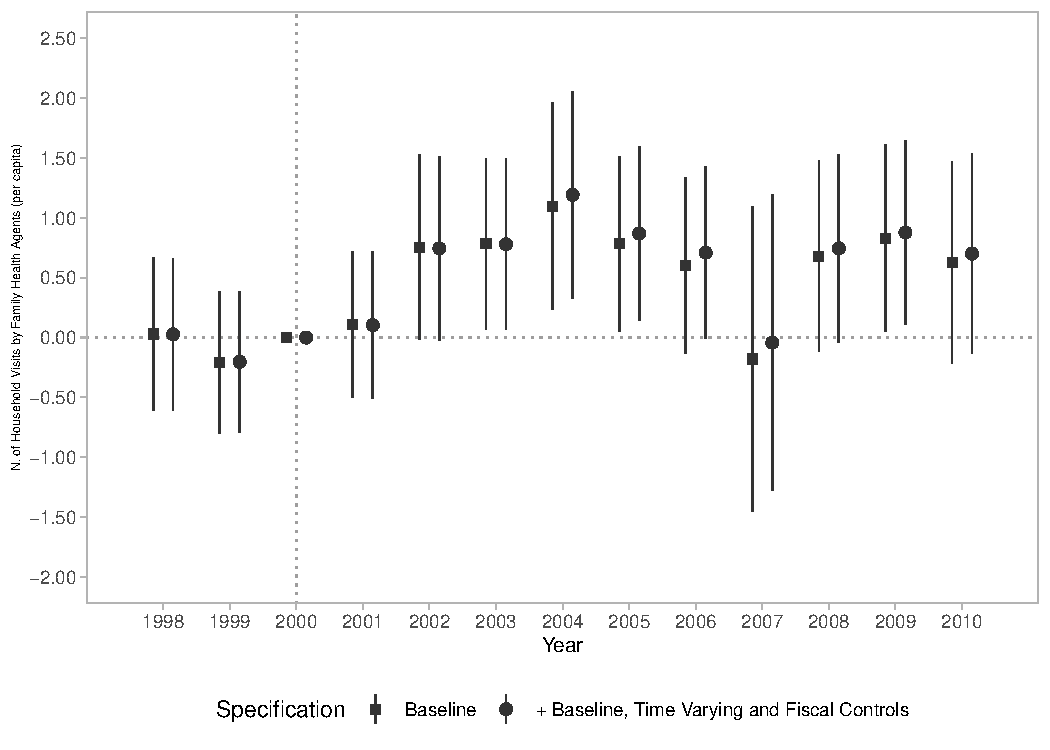
\includegraphics[width=\textwidth]{plots/siab_visit_cha_psf_pcapita_dist_ec29_baseline_dist_ec29_baseline_12.pdf}
    \end{subfigure}
        \begin{subfigure}{0.32\textwidth}
        \caption{\scriptsize N. of Appointments}\label{fig:12g}
        \centering
        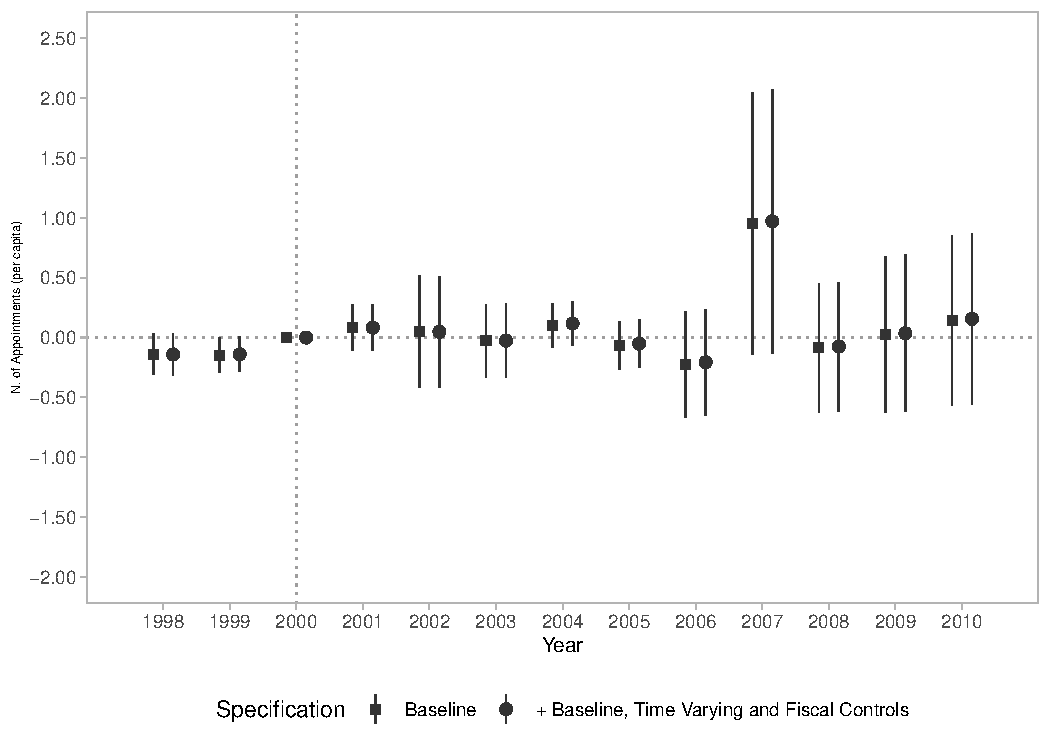
\includegraphics[width=\textwidth]{plots/siab_cons_especif_pcapita_dist_ec29_baseline_dist_ec29_baseline_12.pdf}
    \end{subfigure}
    \begin{subfigure}{0.32\textwidth}
        \centering
        \caption{\scriptsize N. of Appointments from CH Program}\label{fig:12h}
        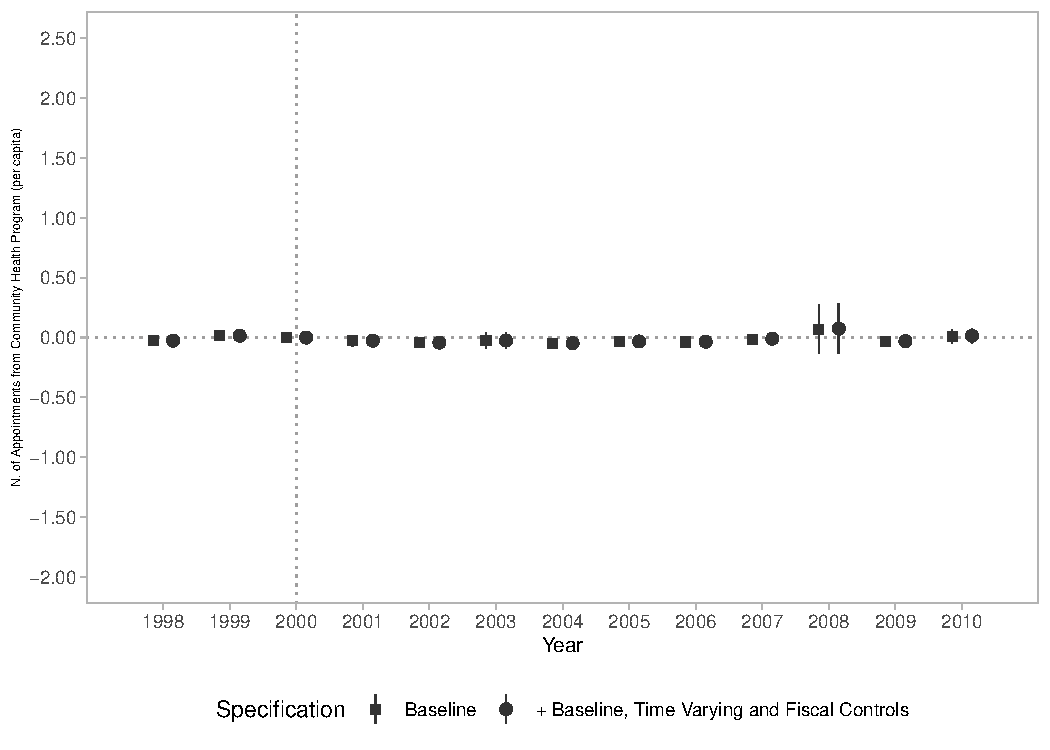
\includegraphics[width=\textwidth]{plots/siab_cons_especif_pacs_pcapita_dist_ec29_baseline_dist_ec29_baseline_12.pdf}
    \end{subfigure}
    \begin{subfigure}{0.32\textwidth}
        \centering
        \caption{\scriptsize N. of Appointments from FH Program}\label{fig:12i}
        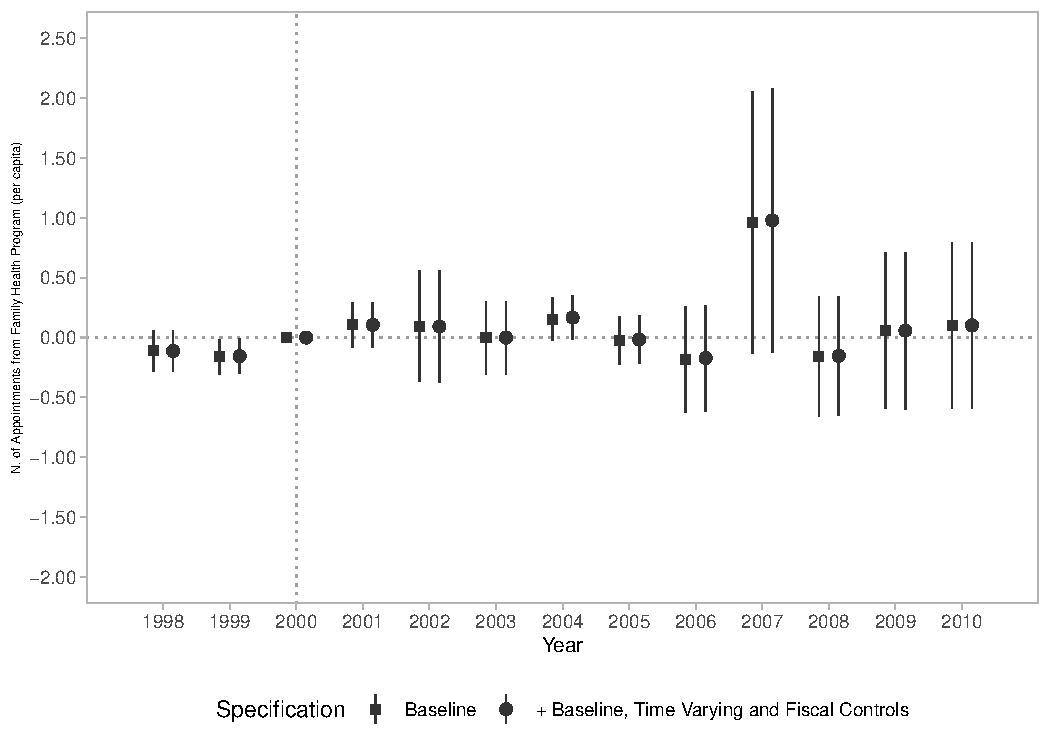
\includegraphics[width=\textwidth]{plots/siab_cons_especif_psf_pcapita_dist_ec29_baseline_dist_ec29_baseline_12.pdf}
    \end{subfigure}
    
    \end{center}
    
\end{figure}

Finally, in Table \ref{table:production} we assess the impacts on ambulatory production and on the access to health services. Panel A show significant effects on the number of outpatient procedures, primary care outpatient procedures and outpatient procedures of low and mid complexity. These point estimates represent a considerably small increase in production, between 2-3\%. We find no significant impact on outpatient procedures of high complexity. The dynamic effects for these outcomes are presented in Figure \ref{fig:14}. In Panel B we present our estimates for the access to health services, measured by prenatal visits. The results show a significant decrease of 0.093 in prenatal visits ignored, that measures under-registration of information on birth records, and a increase of 0.116 in 1 to 6 prenatal visits. These results suggests an improvement in data registration, and considerably small effect on prenatal 1-6. If we consider only the effect beyond the reduction in under-registration, the effect will be equivalent to only 0.4\% increase relative to the baseline for the representative municipality. Figure \ref{fig:13} present the dynamic effects for prenatal visits. Figure \ref{fig:13b} suggests that the EC/29 might have had some effect in reducing the share of births with mothers having no prenatal visits, which could explain this increase in prenatal 1-6 above the reduction in under-registration.

\begin{table}[H]
\begin{footnotesize}
\begin{center}
\scalebox{0.8}{
\begin{threeparttable}[b]

  \centering
  \caption{Ambulatorial Production and Access to Health Services}
     \begin{tabular}{rrrrrr}
          &       &       &       &       &  \\
    \midrule
    \midrule
          &       & \multicolumn{4}{c}{Distance to EC9 target} \\
\cmidrule{3-6}          &       & \multicolumn{1}{c}{(1)} & \multicolumn{1}{c}{(2)} & \multicolumn{1}{c}{(3)} & \multicolumn{1}{c}{(4)} \\
    \midrule
    \multicolumn{1}{p{26.355em}}{\textbf{A. Ambulatorial Production}} &       &       &       &       &  \\
    \multicolumn{1}{l}{\multirow{2}[0]{*}{Outpatient procedures per capita}} &       & \multicolumn{1}{c}{2.67***} & \multicolumn{1}{c}{2.473**} & \multicolumn{1}{c}{2.544**} & \multicolumn{1}{c}{ 2.528** } \\
          &       & \multicolumn{1}{c}{(1.027)} & \multicolumn{1}{c}{(1.025)} & \multicolumn{1}{c}{(1.021)} & \multicolumn{1}{c}{ (1.019) } \\
    \multicolumn{1}{l}{\multirow{2}[0]{*}{Primary Care Outpatient procedures per capita}} &       & \multicolumn{1}{c}{2.231**} & \multicolumn{1}{c}{2.228**} & \multicolumn{1}{c}{2.282**} & \multicolumn{1}{c}{ 2.266** } \\
          &       & \multicolumn{1}{c}{(0.944)} & \multicolumn{1}{c}{(0.934)} & \multicolumn{1}{c}{(0.931)} & \multicolumn{1}{c}{ (0.929) } \\
    \multicolumn{1}{l}{\multirow{2}[0]{*}{N. of Low \& Mid Complexity Outpatient Procedures (per capita)}} &       & \multicolumn{1}{c}{2.337**} & \multicolumn{1}{c}{2.225**} & \multicolumn{1}{c}{2.331***} & \multicolumn{1}{c}{ 2.337*** } \\
          &       & \multicolumn{1}{c}{(0.908)} & \multicolumn{1}{c}{(0.898)} & \multicolumn{1}{c}{(0.892)} & \multicolumn{1}{c}{ (0.891) } \\
    \multicolumn{1}{l}{\multirow{2}[0]{*}{N. of High Complexity Outpatient Procedures (per capita)}} &       & \multicolumn{1}{c}{-0.136} & \multicolumn{1}{c}{-0.191} & \multicolumn{1}{c}{-0.174} & \multicolumn{1}{c}{ -0.177 } \\
          &       & \multicolumn{1}{c}{(0.134)} & \multicolumn{1}{c}{(0.133)} & \multicolumn{1}{c}{(0.132)} & \multicolumn{1}{c}{ (0.132) } \\
    \multicolumn{1}{l}{\multirow{2}[0]{*}{N. of Outpatient Procedures by Low Skilled Workers (per capita)}} &       & \multicolumn{1}{c}{0.04} & \multicolumn{1}{c}{0.019} & \multicolumn{1}{c}{0.074} & \multicolumn{1}{c}{ 0.074 } \\
          &       & \multicolumn{1}{c}{(0.354)} & \multicolumn{1}{c}{(0.346)} & \multicolumn{1}{c}{(0.343)} & \multicolumn{1}{c}{ (0.342) } \\
    \multicolumn{1}{l}{\multirow{2}[0]{*}{N. of Outpatient procedures by Mid Skilled Workers (per capita)}} &       & \multicolumn{1}{c}{0.383} & \multicolumn{1}{c}{0.346} & \multicolumn{1}{c}{0.353} & \multicolumn{1}{c}{ 0.351 } \\
          &       & \multicolumn{1}{c}{(0.481)} & \multicolumn{1}{c}{(0.479)} & \multicolumn{1}{c}{(0.479)} & \multicolumn{1}{c}{ (0.479) } \\
          &       &       &       &       &  \\
    \midrule
    \multicolumn{1}{p{26.355em}}{\textbf{B. Access to Health Services}} &       &       &       &       &  \\
    \multicolumn{1}{l}{\multirow{2}[0]{*}{Prenatal Visits None}} &       & \multicolumn{1}{c}{0.025*} & \multicolumn{1}{c}{0.006} & \multicolumn{1}{c}{0.005} & \multicolumn{1}{c}{0.005} \\
          &       & \multicolumn{1}{c}{(0.015)} & \multicolumn{1}{c}{(0.011)} & \multicolumn{1}{c}{(0.011)} & \multicolumn{1}{c}{(0.011)} \\
    \multicolumn{1}{l}{\multirow{2}[0]{*}{Prenatal Visits 1-6}} &       & \multicolumn{1}{c}{0.13**} & \multicolumn{1}{c}{0.121**} & \multicolumn{1}{c}{0.118*} & \multicolumn{1}{c}{0.116*} \\
          &       & \multicolumn{1}{c}{(0.059)} & \multicolumn{1}{c}{(0.061)} & \multicolumn{1}{c}{(0.061)} & \multicolumn{1}{c}{(0.06)} \\
    \multicolumn{1}{l}{\multirow{2}[0]{*}{Prenatal Visits 7+}} &       & \multicolumn{1}{c}{-0.051} & \multicolumn{1}{c}{-0.034} & \multicolumn{1}{c}{-0.03} & \multicolumn{1}{c}{-0.029} \\
          &       & \multicolumn{1}{c}{(0.074)} & \multicolumn{1}{c}{(0.062)} & \multicolumn{1}{c}{(0.061)} & \multicolumn{1}{c}{(0.061)} \\
          &       &       &       &       &  \\
    \bottomrule
    \bottomrule
    \end{tabular}%
    
    
  \label{table:production}%

\end{threeparttable}
}
\end{center}
\end{footnotesize}
\end{table}

\begin{figure}[h!]
    \begin{center}
    \caption{Effects on Access to Health Services}\label{fig:14}
    \begin{subfigure}{0.32\textwidth}
        \caption{\scriptsize Prenatal Visits None}\label{fig:14a}
        \centering
        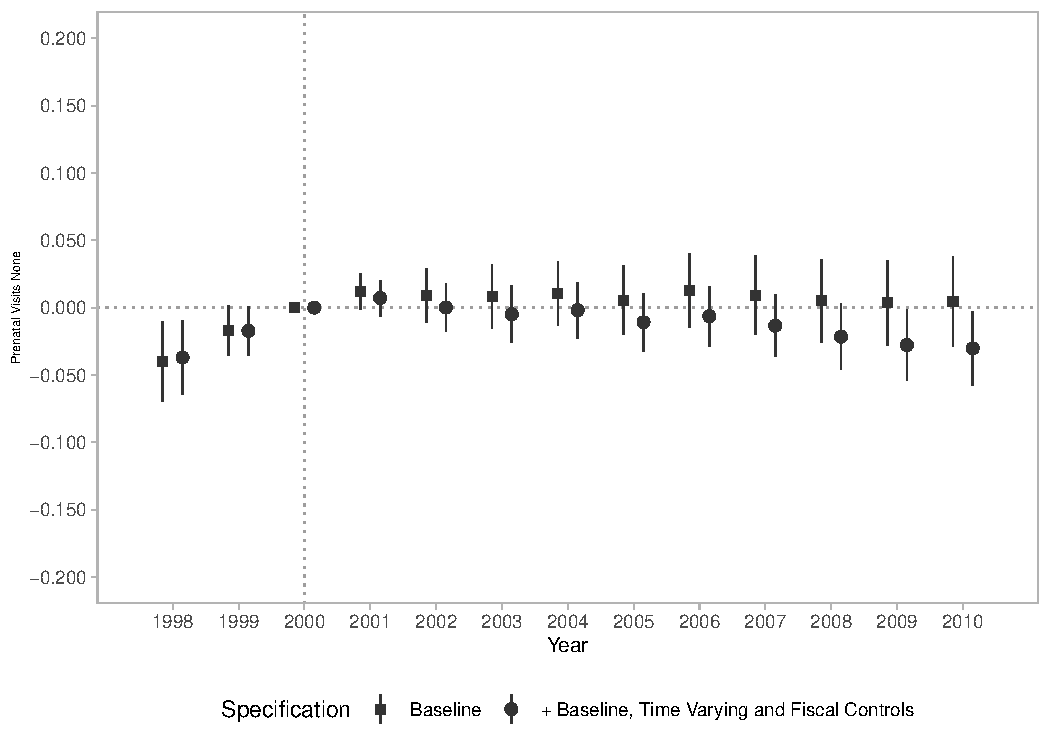
\includegraphics[width=\textwidth]{plots/birth_prenat_0_dist_ec29_baseline_dist_ec29_baseline_14.pdf}
    \end{subfigure}
    \begin{subfigure}{0.32\textwidth}
        \centering
        \caption{\scriptsize Prenatal Visits 1-6}\label{fig:14b}
        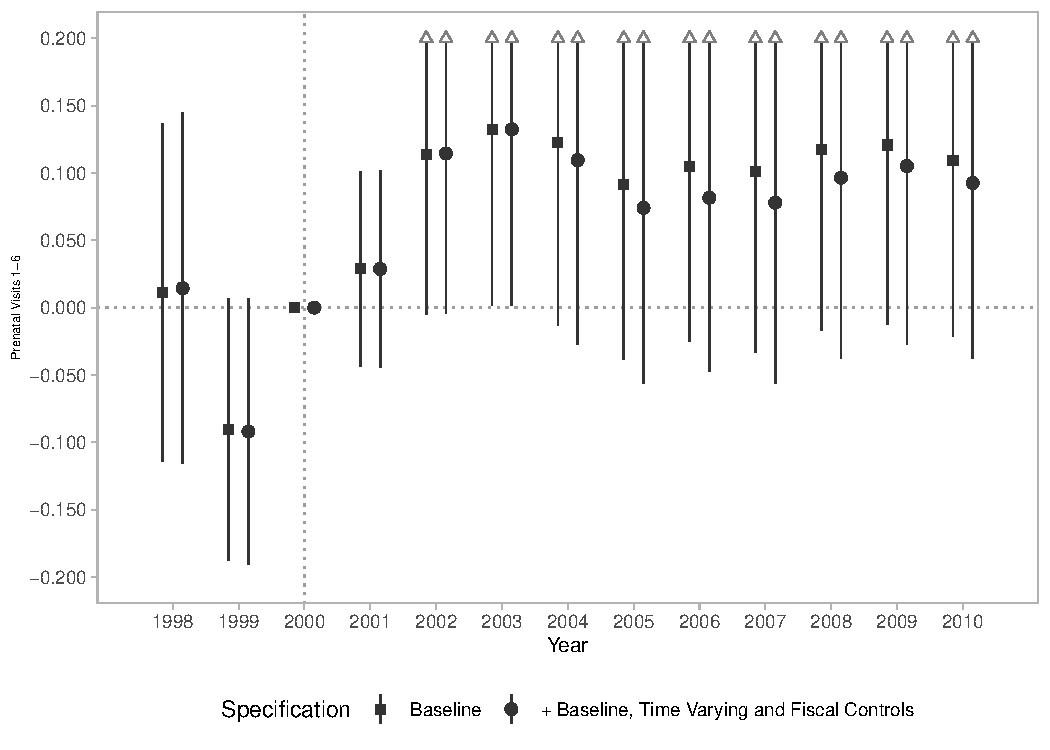
\includegraphics[width=\textwidth]{plots/birth_prenat_1_6_dist_ec29_baseline_dist_ec29_baseline_14.pdf}
    \end{subfigure}
    \begin{subfigure}{0.32\textwidth}
        \centering
        \caption{\scriptsize Prenatal Visits 7+}\label{fig:14c}
        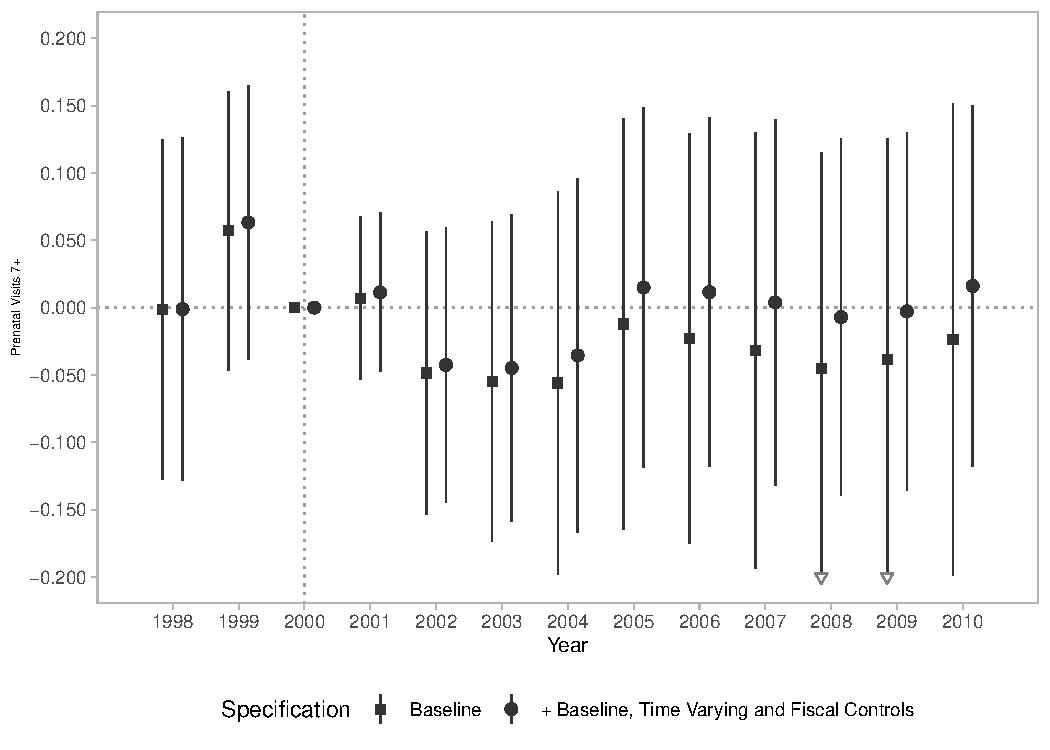
\includegraphics[width=\textwidth]{plots/birth_prenat_7_plus_dist_ec29_baseline_dist_ec29_baseline_14.pdf}
    \end{subfigure}
        
    
    \end{center}
    
\end{figure}

\begin{figure}[h!]
    \begin{center}
    \caption{Effects on Access to Health Services}\label{fig:13}
    \begin{subfigure}{0.48\textwidth}
        \caption{\scriptsize Prenatal Visits Ignored}\label{fig:13a}
        \centering
        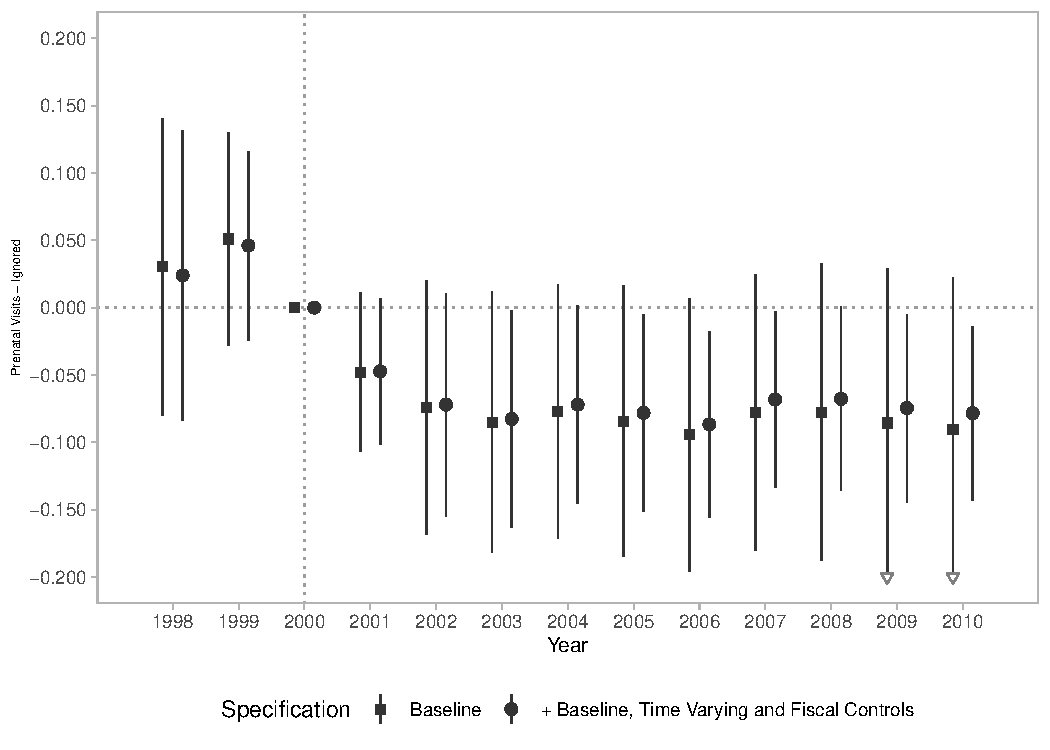
\includegraphics[width=\textwidth]{plots/birth_prenat_ig_dist_ec29_baseline_dist_ec29_baseline_13.pdf}
    \end{subfigure}
    \begin{subfigure}{0.48\textwidth}
        \caption{\scriptsize Prenatal Visits None}\label{fig:13b}
        \centering
        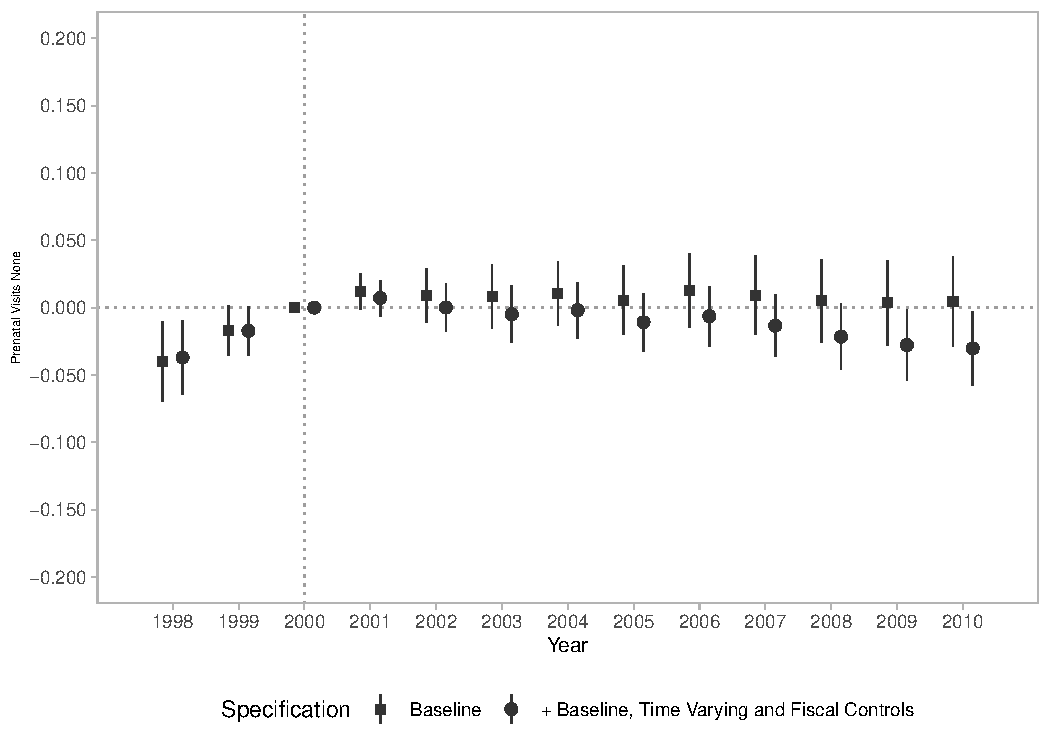
\includegraphics[width=\textwidth]{plots/birth_prenat_0_dist_ec29_baseline_dist_ec29_baseline_13.pdf}
    \end{subfigure}
    \begin{subfigure}{0.48\textwidth}
        \centering
        \caption{\scriptsize Prenatal Visits 1-6}\label{fig:13c}
        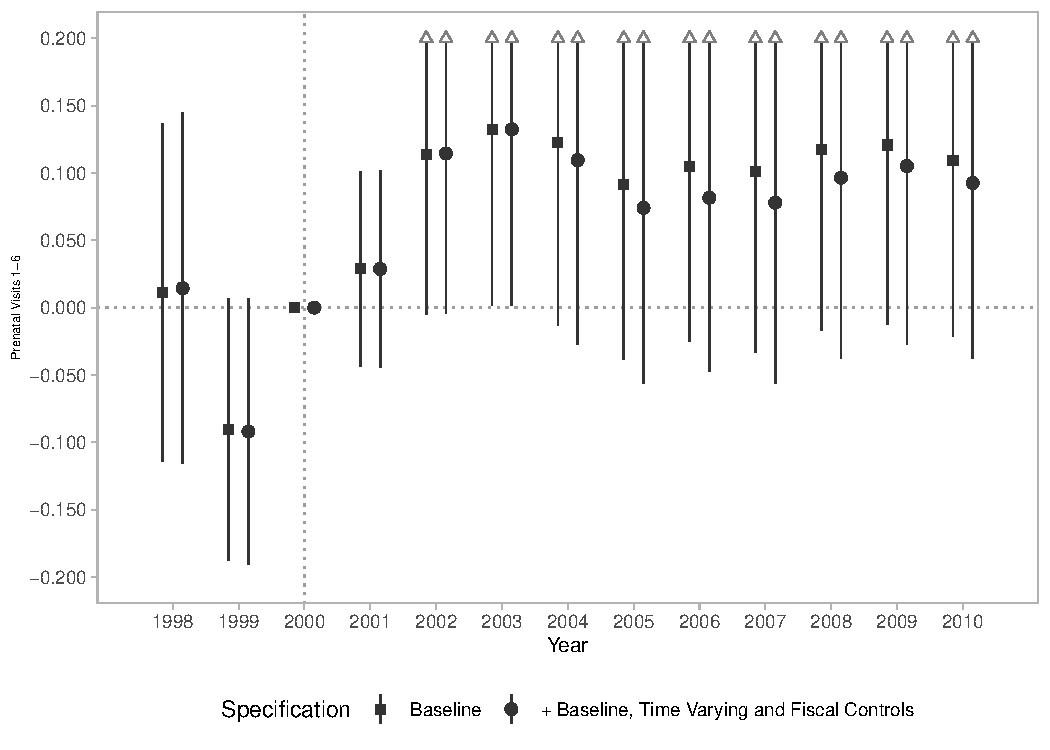
\includegraphics[width=\textwidth]{plots/birth_prenat_1_6_dist_ec29_baseline_dist_ec29_baseline_13.pdf}
    \end{subfigure}
    \begin{subfigure}{0.48\textwidth}
        \centering
        \caption{\scriptsize Prenatal Visits 7+}\label{fig:13d}
        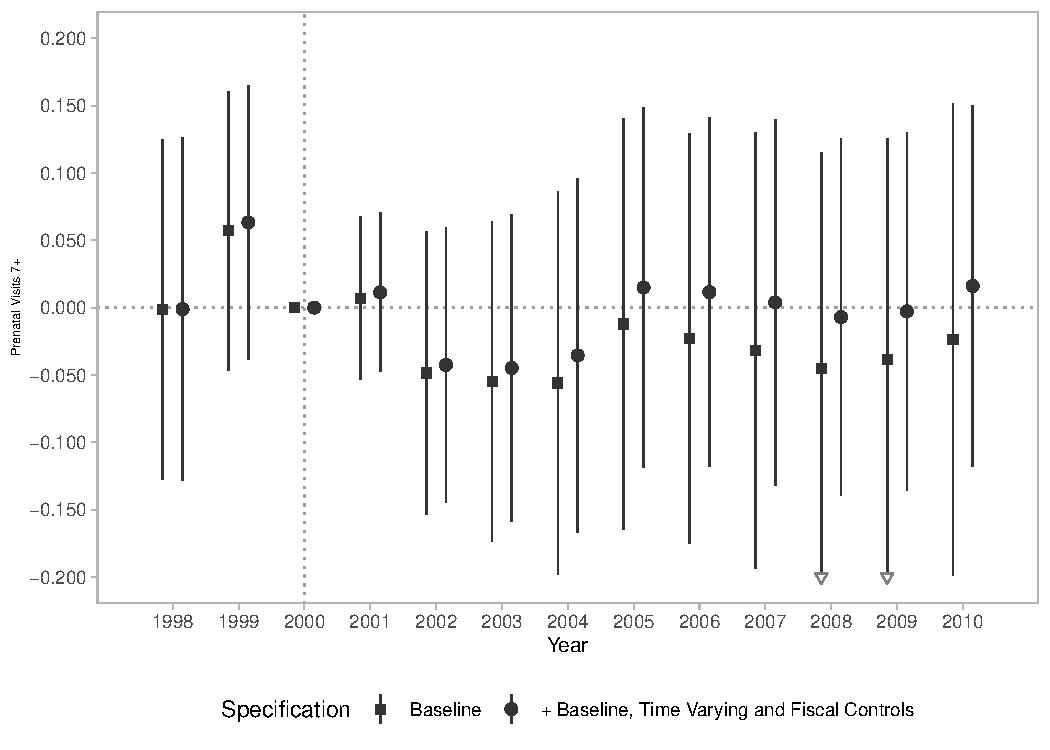
\includegraphics[width=\textwidth]{plots/birth_prenat_7_plus_dist_ec29_baseline_dist_ec29_baseline_13.pdf}
    \end{subfigure}
        
    
    \end{center}
    
    \scriptsize{Notes: The number of observations is 64481. DiD Estimates from Equation \ref{eq:2}. Independent variable is the distance to the EC/29 target in p.p. Square dots represent the baseline model with municipality and state-year fixed effects. Round dots represent fully saturated specification (Column 4 in regression Tables). Lines represent 95\% confidence intervals. Arrows, when present, indicate confidence intervals out of the plot bounds. Standard errors are clustered in the municipality level.}

    
\end{figure}

With the data available we are not able to directly connect the increase in health spending with the increase in health inputs presented in this section. However, the evidence presented so far suggests that: (i) increases in human resource spending have been translated into greater primary care coverage at the intensive margin, a higher number of facilities with primary care personnel, and into a increase in the number of nursing assistants; (ii) increases in investment spending has been translated into a greater supply of municipal hospitals and a marginal increase ambulatory production; and (iii) increases in other expenditures, which consist mainly of administrative spending, might be associated with the increase in the number of administrative professionals.


\subsection{Effects on Infant Mortality}

Having provided meaningful evidence of the effects of EC/29 on health spending and how these effects translated into health inputs, we now present estimates of the effects on infant mortality. Differently from most of the literature linking health spending with infant mortality \citep{filmer1999,bokhari2007,moreno2015,nixon2006,gupta2002effectiveness,cremieux1999,bokhari2007}, we are able to assess the effects not only for total infant mortality rates, but also for infant mortality rates by timing of death and by cause of death. We are also able to analyse infant mortality rates by classifying them between amenable and non-amenable to primary care. These results are presented in Table \ref{table:imr}. In all specifications presented for this section, we added a trend of baseline ill-defined infant mortality with the goal of accounting for mortality under-reporting\footnote{Appendix Table \ref{app:imr} presents estimates with and without the baseline ill-defined infant mortality trend.}. During the period of analysis, the completeness of death counts improved considerably and it is strongly associated with the reduction in ill-defined causes of death \citep{lima2014evolution}.

\begin{table}[h!]
\begin{footnotesize}
\begin{center}
\scalebox{0.9}{
\begin{threeparttable}[b]

  \centering
  \caption{Infant Mortality Rates}
     \begin{tabular}{rrcccc}
          &       &       &       &       &  \\
          &       &       &       &       &  \\
    \midrule
    \midrule
          &       & (1)   & (2)   & (3)   & (4) \\
    \midrule
    \multicolumn{1}{p{15.145em}}{\textbf{A. Infant Mortality Rate}} &       &       &       &       &  \\
    \multicolumn{1}{p{15.145em}}{Total} &       & -5.015 & -3.772 & -3.831 & -3.889 \\
          &       & (3.435) & (2.853) & (2.836) & (2.828) \\
    \multicolumn{1}{p{15.145em}}{Amenable to Primary Care} &       & -0.361 & -0.866 & -0.893 & -0.905 \\
          &       & (0.603) & (0.553) & (0.553) & (0.554) \\
    \multicolumn{1}{p{15.145em}}{Non-Amenable to Primary Care} &       & -4.653 & -2.907 & -2.939 & -2.984 \\
          &       & (3.245) & (2.645) & (2.632) & (2.624) \\
          &       &       &       &       &  \\
    \midrule
    \multicolumn{1}{p{15.145em}}{\textbf{B. By timing}} &       &       &       &       &  \\
    \multicolumn{1}{p{15.145em}}{Fetal} &       & -0.008 & -0.007 & -0.008 & -0.008 \\
          &       & (0.008) & (0.008) & (0.008) & (0.008) \\
    \multicolumn{1}{p{15.145em}}{Within 24h} &       & -2.275* & -2.083** & -2.07** & -2.071** \\
          &       & (1.225) & (0.98) & (0.979) & (0.976) \\
    \multicolumn{1}{p{15.145em}}{1 to 27 days} &       & -4.228* & -2.883 & -2.911 & -2.922 \\
          &       & (2.555) & (2.064) & (2.052) & (2.046) \\
    \multicolumn{1}{p{15.145em}}{27 days to 1 year} &       & -0.787 & -0.89 & -0.92 & -0.967 \\
          &       & (1.435) & (1.248) & (1.246) & (1.243) \\
          &       &       &       &       &  \\
    \midrule
    \multicolumn{1}{p{15.145em}}{\textbf{C. By Cause of Death}} &       &       &       &       &  \\
    \multicolumn{1}{p{15.145em}}{Infectious} &       & -0.374 & -0.811 & -0.82 & -0.831 \\
          &       & (0.567) & (0.535) & (0.535) & (0.534) \\
    \multicolumn{1}{p{15.145em}}{Respiratory} &       & -0.494 & -0.507 & -0.511 & -0.517 \\
          &       & (0.474) & (0.411) & (0.409) & (0.409) \\
    \multicolumn{1}{p{15.145em}}{Perinatal} &       & -5.349** & -3.648* & -3.69* & -3.707* \\
          &       & (2.571) & (2.015) & (2.007) & (2.002) \\
    \multicolumn{1}{p{15.145em}}{Congenital} &       & -0.235 & -0.169 & -0.16 & -0.157 \\
          &       & (0.463) & (0.436) & (0.434) & (0.434) \\
    \multicolumn{1}{p{15.145em}}{External} &       & 0.024 & -0.049 & -0.037 & -0.034 \\
          &       & (0.183) & (0.165) & (0.165) & (0.166) \\
    \multicolumn{1}{p{15.145em}}{Nutritional} &       & -0.204 & -0.328 & -0.33 & -0.343 \\
          &       & (0.246) & (0.231) & (0.232) & (0.232) \\
    \multicolumn{1}{p{15.145em}}{Other} &       & -0.183 & -0.123 & -0.132 & -0.139 \\
          &       & (0.201) & (0.199) & (0.198) & (0.198) \\
    \multicolumn{1}{p{15.145em}}{Ill-Defined} &       & 1.8** & 1.862** & 1.849** & 1.84** \\
          &       & (0.849) & (0.776) & (0.779) & (0.779) \\
          &       &       &       &       &  \\
    \bottomrule
    \bottomrule
    \end{tabular}%
    
    
    \begin{tablenotes}
  \scriptsize{\underline{Notes}: The number of observations is 64482. DiD Estimates from Equation \ref{eq:1}. Independent variable is the distance to the EC/29 target in p.p. Column 1 presents the baseline model with municipality and state-year fixed effects. Column 2 adds baseline socioeconomic controls from the Census interacted with time. Column 3 adds controls for GDP per capita and \emph{Bolsa Familia} transfers per capita. Column 4 adds fiscal controls. Covariates omitted. Standard errors in brackets are clustered in the municipality level. ∗p < 0.10, ∗ ∗ p < 0.05, ∗ ∗ ∗p < 0.01}
  \end{tablenotes}
    
    
  \label{table:imr}%

\end{threeparttable}
}
\end{center}
\end{footnotesize}
\end{table}

Panel A present the estimates for total infant mortality rates (IMR) and IMR amenable and non-amenable to primary care. Though not significant, the estimates present the expected sign. Yet, the more flexible coefficients estimated with equation \ref{eq:2} provide useful information on the dynamics of the effects and suggest the presence of some significant reduction in IMR. Figure \ref{fig:15} plots the dynamic effects for the IMR presented in Panel A. IMR (Figure \ref{fig:15a}) and IMR amenable to primary care (Figure \ref{fig:15b})  present a clear trend of reduction, with estimates for 2007 onward being all statistically significant in our preferred specification. 

\begin{figure}[h!]
    \begin{center}
    \caption{Effects on Infant Mortality Rates}\label{fig:15}
    \begin{subfigure}{0.32\textwidth}
        \caption{\scriptsize Total}\label{fig:15a}
        \centering
        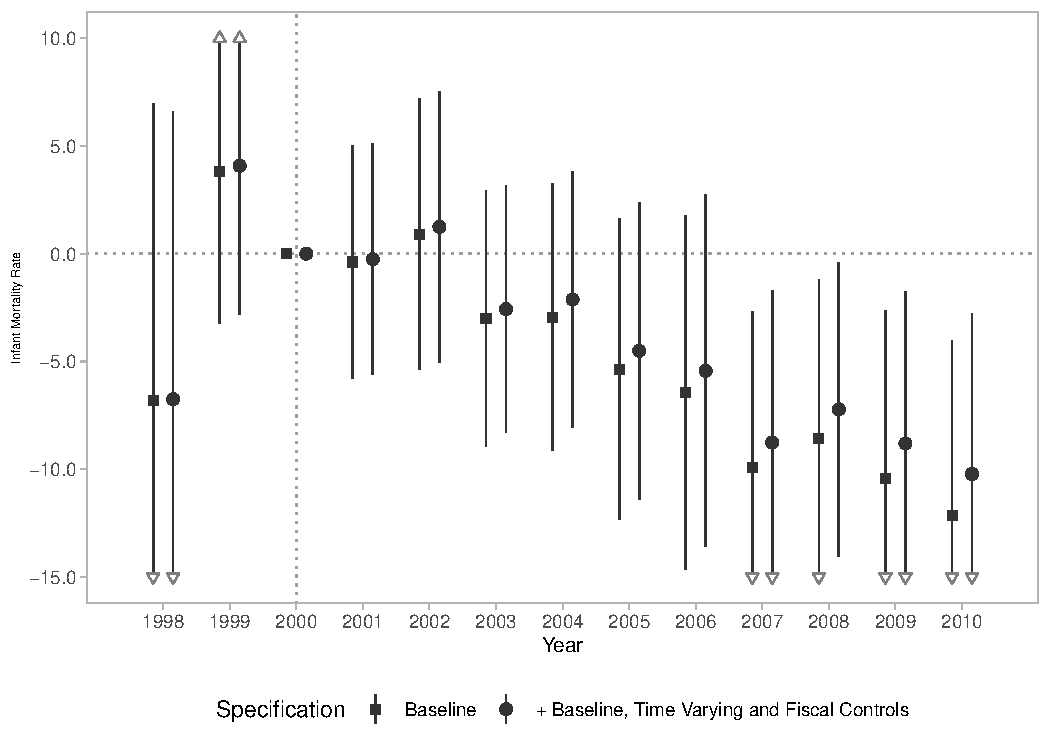
\includegraphics[width=\textwidth]{plots/tx_mi_dist_ec29_baseline_dist_ec29_baseline_15.pdf}
    \end{subfigure}
    \begin{subfigure}{0.32\textwidth}
        \centering
        \caption{\scriptsize Amenable to Primary Care}\label{fig:15b}
        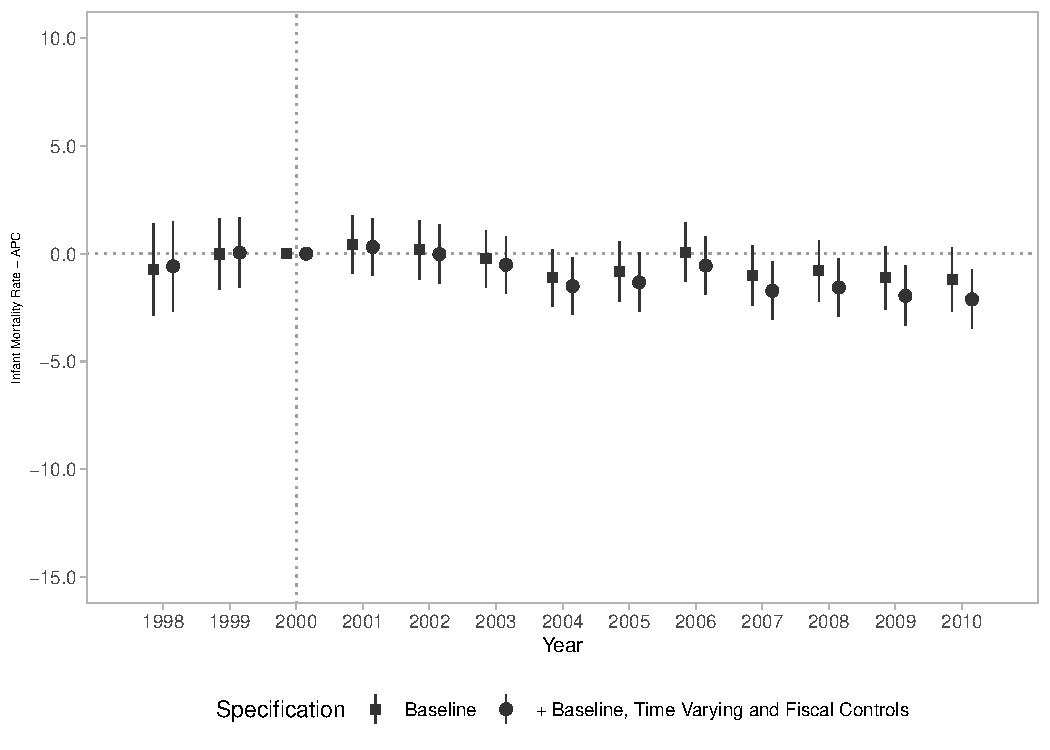
\includegraphics[width=\textwidth]{plots/tx_mi_icsap_dist_ec29_baseline_dist_ec29_baseline_15.pdf}
    \end{subfigure}
    \begin{subfigure}{0.32\textwidth}
        \centering
        \caption{\scriptsize Non-Amenable to Primary Care}\label{fig:15c}
        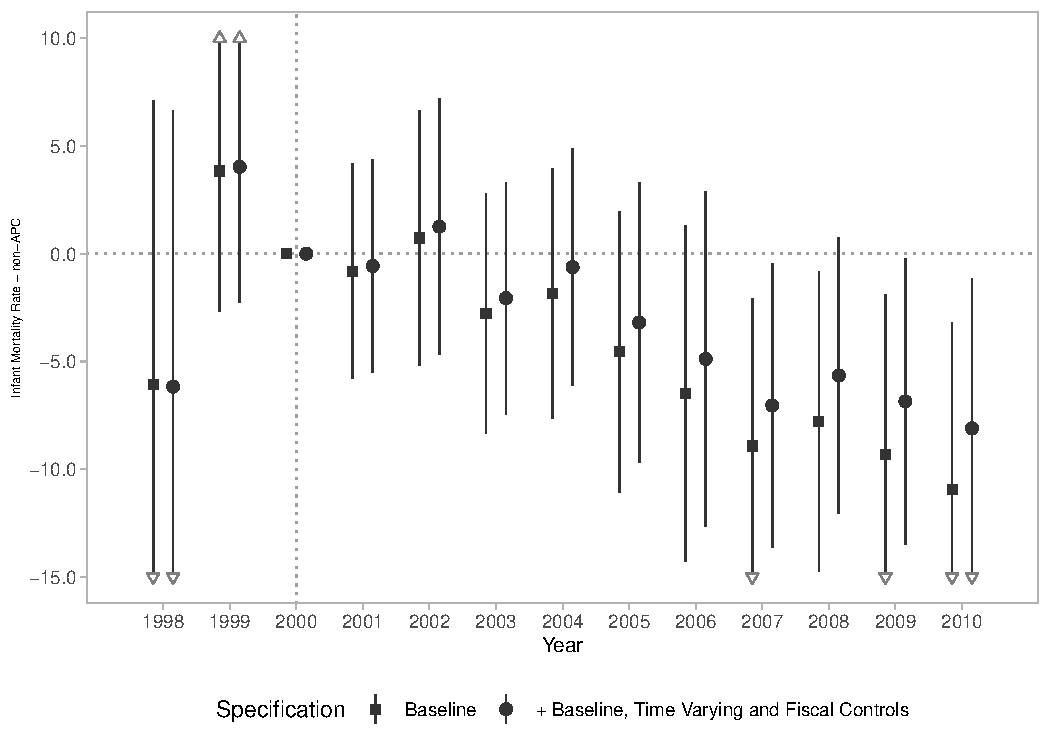
\includegraphics[width=\textwidth]{plots/tx_mi_nicsap_dist_ec29_baseline_dist_ec29_baseline_15.pdf}
    \end{subfigure}
    
    \end{center}
    
        \scriptsize{Notes: The number of observations is 64482. DiD Estimates from Equation \ref{eq:2}. Independent variable is the distance to the EC/29 target in p.p. Square dots represent the baseline model with municipality and state-year fixed effects. Round dots represent fully saturated specification (Column 4 in regression Tables). Lines represent 95\% confidence intervals. Arrows, when present, indicate confidence intervals out of the plot bounds. Standard errors are clustered in the municipality level.}
    
\end{figure}

Next, we present the estimates for IMR by timing of death (Panel B). IMR withing 24 hours shows a significant reduction of 2.071, which is equivalent to a 3.7\% decreased in baseline mortality for the representative municipality. The estimates for the remaining IMR of Panel B are not significant, but the dynamic effects suggests the presence of reduction trend in later years for IMR from 1 to 27 days (Figure \ref{fig:16c}) and IMR from 27 days to 1 year old (Figure \ref{fig:16d}).

\begin{figure}[h!]
    \begin{center}
    \caption{Effects on Infant Mortality Rates - By Timing}\label{fig:16}
    \begin{subfigure}{0.48\textwidth}
        \caption{\scriptsize Fetal}\label{fig:16a}
        \centering
        \includegraphics[width=\textwidth]{plots/tx_mi_fet_dist_ec29_baseline_dist_ec29_baseline_16.pdf}
    \end{subfigure}
    \begin{subfigure}{0.48\textwidth}
        \centering
        \caption{\scriptsize Within 24h}\label{fig:16b}
        \includegraphics[width=\textwidth]{plots/tx_mi_24h_dist_ec29_baseline_dist_ec29_baseline_16.pdf}
    \end{subfigure}
    \begin{subfigure}{0.48\textwidth}
        \centering
        \caption{\scriptsize 1 to 27 days}\label{fig:16c}
        \includegraphics[width=\textwidth]{plots/tx_mi_27d_dist_ec29_baseline_dist_ec29_baseline_16.pdf}
    \end{subfigure}
    \begin{subfigure}{0.48\textwidth}
        \centering
        \caption{\scriptsize 27 days to 1 year}\label{fig:16d}
        \includegraphics[width=\textwidth]{plots/tx_mi_ano_dist_ec29_baseline_dist_ec29_baseline_16.pdf}
    \end{subfigure}
    
    \end{center}
    
            \scriptsize{Notes: The number of observations is 64482. DiD Estimates from Equation \ref{eq:2}. Independent variable is the distance to the EC/29 target in p.p. Square dots represent the baseline model with municipality and state-year fixed effects. Round dots represent fully saturated specification (Column 4 in regression Tables). Lines represent 95\% confidence intervals. Arrows, when present, indicate confidence intervals out of the plot bounds. Standard errors are clustered in the municipality level.}
    
\end{figure}

The last part of Table \ref{table:imr} present the estimates for IMR by causes of death. We only find marginally significant reductions for IMR from Perinatal causes. This estimated represents a 3.4\% decrease relative to baseline mortality. We also find the unexpected effect of increases in IMR from ill-defined causes. Moreover, the dynamic effects presented in Figure \ref{fig:17} suggest the presence of some reduction in IMR by infectious and in IMR by respiratory causes.

In our preferred specification, with the exception of ill-defined infant mortality, all outcomes present negative point estimates, but only infant mortality rate within 24 hours and infant mortality rate by infectious diseases present marginally significant estimates. Relative to the baseline mortality rates, a 10\% distance to the target is associated with a reduction of around 3.5\% for mortality within 24 hours and a reduction of around 5\% for mortality due to infectious diseases. 

\begin{figure}[h!]
    \begin{center}
    \caption{Effects on Infant Mortality Rates - By Timing}\label{fig:17}
    \begin{subfigure}{0.48\textwidth}
        \caption{\scriptsize Fetal}\label{fig:17a}
        \centering
        \includegraphics[width=\textwidth]{plots/tx_mi_fet_dist_ec29_baseline_dist_ec29_baseline_17.pdf}
    \end{subfigure}
    \begin{subfigure}{0.48\textwidth}
        \centering
        \caption{\scriptsize Within 24h}\label{fig:17b}
        \includegraphics[width=\textwidth]{plots/tx_mi_24h_dist_ec29_baseline_dist_ec29_baseline_17.pdf}
    \end{subfigure}
    \begin{subfigure}{0.48\textwidth}
        \centering
        \caption{\scriptsize 1 to 27 days}\label{fig:17c}
        \includegraphics[width=\textwidth]{plots/tx_mi_27d_dist_ec29_baseline_dist_ec29_baseline_17.pdf}
    \end{subfigure}
    \begin{subfigure}{0.48\textwidth}
        \centering
        \caption{\scriptsize 27 days to 1 year}\label{fig:17d}
        \includegraphics[width=\textwidth]{plots/tx_mi_ano_dist_ec29_baseline_dist_ec29_baseline_17.pdf}
    \end{subfigure}
    
    \end{center}
    
\end{figure}

In general, articles estimating the causal relationship between health spending and mortality run log-log regressions and present estimates for the elasticity of mortality with respect to health spending. We explicitly choose not to apply transformations to our health outcomes variables due to the amount of observations with values equal to $0$, notably the ones related to birth and mortality. Our data comprises all the Brazilian municipalities with available data for the period of analyses, some with population size as little as $700$ inhabitants, and it is common to find infant mortality rates of $0$. Running log transformation would throw away some relevant information for several outcomes. Nonetheless, to relate our results to the literature on this topic we estimate "back of the envelope" elasticities for all IMR using the estimates of our regressions. Table \ref{table:elasticity} presents these elasticities. 

The elasticities presented in the literature vary greatly. Within cross-country studies, while \cite{filmer1999} finds a very small elasticity of $-0.08$, \cite{gupta2002effectiveness} finds an elasticity of $-0.31$ and \cite{bokhari2007} elasticities ranging between $-0.4$ and $-0.5$. In the micro studies \cite{cremieux1999} finds large elasticities between $-0.8$ and $-1.1$, \cite{sonia2007} finds an elasticity of $-0.24$ for rural regions, and \cite{castro2021effects} elasticities ranging between $-0.5$ and $-0.9$. Though not significant, our study finds much smaller elasticities for total infant mortality rates. Using SIOPS as the measure of health spending, we find IMR elasticities ranging between $-0.06$ and $-0.14$. When it comes to within 24 hours IMR and Perinatal IMR, the rates for which we found significant decreases, the back of the envelope calculations suggest an elasticity of $-0.136$ and $-0.124$, respectively.


\begin{table}[h!]
\begin{footnotesize}
\begin{center}
\scalebox{0.8}{
\begin{threeparttable}[b]

  \centering
  \caption{Fertility and Birth Outcomes}
     \begin{tabular}{rrcccr}
          &       &       &       &       &  \\
          &       &       &       &       &  \\
    \midrule
    \midrule
          &       & (1)   & (2)   & (3)   & \multicolumn{1}{c}{(4)} \\
    \midrule
    \multicolumn{1}{l}{\textbf{A. Fertility}} &       &       &       &       &  \\
    \multicolumn{1}{p{26.355em}}{Rates of Birth per Woman (10-49y)} &       & 0.009** & 0.008** & 0.009** & \multicolumn{1}{c}{ 0.009** } \\
          &       & (0.004) & (0.003) & (0.003) & \multicolumn{1}{c}{ (0.003) } \\
    \multicolumn{1}{p{26.355em}}{\textbf{B. Birth Outcomes}} &       &       &       &       &  \\
    \multicolumn{1}{p{26.355em}}{Apgar 1} &       & -0.056 & 0.063 & 0.053 & \multicolumn{1}{c}{ 0.051 } \\
          &       & (0.206) & (0.198) & (0.198) & \multicolumn{1}{c}{ (0.198) } \\
    \multicolumn{1}{p{26.355em}}{Apgar 5} &       & 0.009 & 0.107 & 0.104 & \multicolumn{1}{c}{ 0.101 } \\
          &       & (0.183) & (0.179) & (0.18) & \multicolumn{1}{c}{ (0.179) } \\
    \multicolumn{1}{p{26.355em}}{Low Birth Weight (<2.5k)} &       & -0.003 & -0.002 & -0.001 & \multicolumn{1}{c}{ -0.002 } \\
          &       & (0.003) & (0.003) & (0.003) & \multicolumn{1}{c}{ (0.003) } \\
    \multicolumn{1}{p{26.355em}}{Premature Birth} &       & -0.005 & -0.016 & -0.017 & \multicolumn{1}{c}{ -0.017 } \\
          &       & (0.026) & (0.023) & (0.023) & \multicolumn{1}{c}{ (0.023) } \\
    \multicolumn{1}{p{26.355em}}{Sex Ratio at Birth} &       & 0.014 & 0.016 & 0.017 & \multicolumn{1}{c}{ 0.017 } \\
          &       & (0.016) & (0.016) & (0.016) & \multicolumn{1}{c}{ (0.016) } \\
          &       &       &       &       &  \\
    \bottomrule
    \bottomrule
    \end{tabular}%
    
    
    \begin{tablenotes}
  \scriptsize{\underline{Notes}: The number of observations is 64482 for Panel A, 63705 for Apgar 1, 59524 for Apgar 5, 64481 for Low Birth Weight and Premature Birth, and 64470 for Sex Ratio at Birth. DiD Estimates from Equation \ref{eq:1}. Independent variable is the distance to the EC/29 target in p.p. Column 1 presents the baseline model with municipality and state-year fixed effects. Column 2 adds baseline socioeconomic controls from the Census interacted with time. Column 3 adds controls for GDP per capita and \emph{Bolsa Familia} transfers per capita. Column 4 adds fiscal controls. Covariates omitted. Standard errors in brackets are clustered in the municipality level. ∗p < 0.10, ∗ ∗ p < 0.05, ∗ ∗ ∗p < 0.011}
  \end{tablenotes}
    
    
  \label{table:birth}%

\end{threeparttable}
}
\end{center}
\end{footnotesize}
\end{table}

Lastly, table \ref{table:birth} presents the estimates for fertility and birth outcomes. In general, the point estimates are in the expected direction, substantially small,but and statistically insignificant. An exception is our measure of fertility that presents small but significant estimates. A 0.009 increase in the fertility rate, correspond to a 1.6\% variation relative to the baseline for the representative municipality. Figure \ref{fig:18} plots the dynamic effects for fertility and birth outcomes. Figure \ref{fig:18a} suggests the presence of some trend in our fertility measure, that seems to show a constant increase from the pre-treatment period until the last year of analysis.

\begin{figure}[h!]
    \begin{center}
    \caption{Effects on Infant Mortality Rates - By Cause}\label{fig:18}
    \begin{subfigure}{0.32\textwidth}
        \caption{\scriptsize Infectious}\label{fig:18a}
        \centering
        \includegraphics[width=\textwidth]{plots/tx_mi_infec_dist_ec29_baseline_dist_ec29_baseline_18.pdf}
    \end{subfigure}
    \begin{subfigure}{0.32\textwidth}
        \centering
        \caption{\scriptsize Respiratory}\label{fig:18b}
        \includegraphics[width=\textwidth]{plots/tx_mi_resp_dist_ec29_baseline_dist_ec29_baseline_18.pdf}
    \end{subfigure}
    \begin{subfigure}{0.32\textwidth}
        \centering
        \caption{\scriptsize Perinatal}\label{fig:18c}
        \includegraphics[width=\textwidth]{plots/tx_mi_perinat_dist_ec29_baseline_dist_ec29_baseline_18.pdf}
    \end{subfigure}
        \begin{subfigure}{0.32\textwidth}
        \centering
        \caption{\scriptsize Congenital}\label{fig:18d}
        \includegraphics[width=\textwidth]{plots/tx_mi_cong_dist_ec29_baseline_dist_ec29_baseline_18.pdf}
    \end{subfigure}
        \begin{subfigure}{0.32\textwidth}
        \centering
        \caption{\scriptsize External}\label{fig:18e}
        \includegraphics[width=\textwidth]{plots/tx_mi_ext_dist_ec29_baseline_dist_ec29_baseline_18.pdf}
    \end{subfigure}
        \begin{subfigure}{0.32\textwidth}
        \centering
        \caption{\scriptsize Nutritional}\label{fig:18f}
        \includegraphics[width=\textwidth]{plots/tx_mi_nut_dist_ec29_baseline_dist_ec29_baseline_18.pdf}
    \end{subfigure}
        \begin{subfigure}{0.32\textwidth}
        \centering
        \caption{\scriptsize Other}\label{fig:18g}
        \includegraphics[width=\textwidth]{plots/tx_mi_out_dist_ec29_baseline_dist_ec29_baseline_18.pdf}
    \end{subfigure}
        \begin{subfigure}{0.32\textwidth}
        \centering
        \caption{\scriptsize Ill-defined}\label{fig:18h}
        \includegraphics[width=\textwidth]{plots/tx_mi_illdef_dist_ec29_baseline_dist_ec29_baseline_18.pdf}
    \end{subfigure}
    \end{center}
    
\end{figure}


Overall, we found significant effects for infant moralities rates that are mainly associated with increases in access to primary care and community-based health interventions \citep{rocha2010evaluating,bhalotra2019can}, suggesting that the effects found for health inputs related to primary care might be the channel through which spending affected infant mortality.


\subsection{Robustness}

In Section \ref{sec:emp_val} we stressed that the validity of our research design relies on having parallel trends and homogeneity in treatment effect. However, we can only empirically test the first identification hypothesis. For all outcomes discussed in this article, we presented figures plotting the estimates of Equation \ref{eq:2} that captures pre-trends in the outcome variable. With only few exceptions, our estimates show no pre-trends in our outcomes.

Another concern may arise from unobserved events coinciding the approval of the EC/29. The inclusion of state-year fixed effects in all specification helps address this concern, as well as the concern on pre-trends. Moreover, we presented in all regression tables estimates for four specifications that gradually included different set of controls, with figures plotting estimates only for the baseline specification and the more complete specification. Our analysis shows that estimates for health spending and health inputs are highly robust to different specifications. The estimates for outcomes related to birth and mortality are a bit more sensible to the inclusion of baseline controls, but still very robust to different specifications.

\section{Conclusions}\label{sec:conclusion}
\setstretch{1.5}

Our empirical analysis has demonstrated that when municipalities are induced to increase public health spending they do so by increasing mainly spending relative to the administrative structure of public health - roughly half of the increase -  followed by spending with investments and human resources. We also demonstrate that this increase is associated with a higher number of administrative professionals, greater supply of municipal hospitals, and greater primary care coverage at the intensive margin, with also a higher number of health facilities with primary care related professionals. The shifts in spending and health inputs are associated with small to moderate reductions in infant mortality rates related to improvements in primary care access, and long term reductions in total infant mortality rates. \cite{bhalotra2019can} have shown that the combination of access to primary and hospital care leads to better health outcomes relative to only primary care. This is a plausible channel through which the increase in the supply of municipal hospitals might be affecting infant mortality in our analysis.

These results are extremely relevant, specially in a context of a universal an decentralized health system, where provision of health care occurs mainly at the municipal level, and the majority of the resources spent locally comes from local tax incomes, in opposition to intergovernmental transfers. [Discuss transfers vs own resource spending]. We are not able to formally test exactly how health inputs and outcomes would react if municipalities allocated less resources on administrative structure and more resources into investments and personnel, but the evidence here present indicates it could lead to further improvements in health outcomes, and, thus, a more efficient use of resources within the public health sector. 


\clearpage
\pagebreak
\singlespacing  
\bibliographystyle{apalike}
\bibliography{SRC}
\nocite{}




\pagebreak
\appendix
\singlespacing	

\LARGE{\textbf{Appendix}}


\counterwithin{figure}{section}
\counterwithin{table}{section}



\section{Descriptive Statistics}\label{app:stats}

\begin{table}[H]
\begin{footnotesize}
\begin{center}
\scalebox{0.8}{
\begin{threeparttable}[b]

  \centering
  \caption{Descriptive Statistics (at the baseline year)}
    
    \begin{tabular}{rrrrrrrr}
          &       &       &       &       &       &       &  \\
    \midrule
    \midrule
          & \multicolumn{1}{c}{Mean} & \multicolumn{1}{c}{Std. Dev.} & \multicolumn{1}{c}{Min} & \multicolumn{1}{c}{Max} & \multicolumn{1}{c}{Obs.} &       & \multicolumn{1}{c}{Source of Data} \\
\cmidrule{1-6}\cmidrule{8-8}    \multicolumn{1}{l}{\textbf{EC 29 Variables}} &       &       &       &       &       &       &  \\
    \multicolumn{1}{l}{Share of Municipality's Own Resource Spent in Public Health} & \multicolumn{1}{c}{0.14} & \multicolumn{1}{c}{0.07} & \multicolumn{1}{c}{0.00} & \multicolumn{1}{c}{0.80} & \multicolumn{1}{c}{5224} &       & \multicolumn{1}{c}{Datasus/SIOPS} \\
    \multicolumn{1}{l}{Distance to the EC29 Target} & \multicolumn{1}{c}{0.01} & \multicolumn{1}{c}{0.07} & \multicolumn{1}{c}{-0.65} & \multicolumn{1}{c}{0.15} & \multicolumn{1}{c}{5224} &       & \multicolumn{1}{c}{Datasus/SIOPS} \\
          &       &       &       &       &       &       &  \\
    \multicolumn{1}{l}{\textbf{Public Revenue}} &       &       &       &       &       &       &  \\
    \multicolumn{1}{l}{Total Revenue per capita} & \multicolumn{1}{c}{1225.27} & \multicolumn{1}{c}{2282.13} & \multicolumn{1}{c}{132.39} & \multicolumn{1}{c}{\#\#\#\#\#\#\#\#} & \multicolumn{1}{c}{5288} &       & \multicolumn{1}{c}{Finbra} \\
          &       &       &       &       &       &       &  \\
    \multicolumn{1}{l}{\textbf{Public Spending}} &       &       &       &       &       &       &  \\
    \multicolumn{1}{l}{Total Spending per capita} & \multicolumn{1}{c}{1284.77} & \multicolumn{1}{c}{2395.06} & \multicolumn{1}{c}{129.74} & \multicolumn{1}{c}{\#\#\#\#\#\#\#\#} & \multicolumn{1}{c}{5304} &       & \multicolumn{1}{c}{Finbra} \\
          &       &       &       &       &       &       &  \\
    \multicolumn{1}{l}{Spending by Type - per capita} &       &       &       &       &       &       &  \\
    \multicolumn{1}{l}{Human Resources} & \multicolumn{1}{c}{502.32} & \multicolumn{1}{c}{985.60} & \multicolumn{1}{c}{0.00} & \multicolumn{1}{c}{60697.09} & \multicolumn{1}{c}{5304} &       & \multicolumn{1}{c}{Finbra} \\
    \multicolumn{1}{l}{Investment} & \multicolumn{1}{c}{153.70} & \multicolumn{1}{c}{277.13} & \multicolumn{1}{c}{0.00} & \multicolumn{1}{c}{14815.46} & \multicolumn{1}{c}{5304} &       & \multicolumn{1}{c}{Finbra} \\
    \multicolumn{1}{l}{Other} & \multicolumn{1}{c}{628.75} & \multicolumn{1}{c}{1280.34} & \multicolumn{1}{c}{0.00} & \multicolumn{1}{c}{79994.44} & \multicolumn{1}{c}{5304} &       & \multicolumn{1}{c}{Finbra} \\
          &       &       &       &       &       &       &  \\
    \multicolumn{1}{l}{Spending by Category - per capita} &       &       &       &       &       &       &  \\
    \multicolumn{1}{l}{Health and Sanitation} & \multicolumn{1}{c}{217.08} & \multicolumn{1}{c}{276.14} & \multicolumn{1}{c}{0.04} & \multicolumn{1}{c}{12559.61} & \multicolumn{1}{c}{5286} &       & \multicolumn{1}{c}{Finbra} \\
    \multicolumn{1}{l}{Transport} & \multicolumn{1}{c}{91.55} & \multicolumn{1}{c}{138.28} & \multicolumn{1}{c}{0.00} & \multicolumn{1}{c}{5865.79} & \multicolumn{1}{c}{5304} &       & \multicolumn{1}{c}{Finbra} \\
    \multicolumn{1}{l}{Education and Culture} & \multicolumn{1}{c}{419.95} & \multicolumn{1}{c}{640.29} & \multicolumn{1}{c}{0.00} & \multicolumn{1}{c}{36319.15} & \multicolumn{1}{c}{5304} &       & \multicolumn{1}{c}{Finbra} \\
    \multicolumn{1}{l}{Housing and Urban} & \multicolumn{1}{c}{116.05} & \multicolumn{1}{c}{301.25} & \multicolumn{1}{c}{0.00} & \multicolumn{1}{c}{19842.15} & \multicolumn{1}{c}{5304} &       & \multicolumn{1}{c}{Finbra} \\
    \multicolumn{1}{l}{Social Assistance} & \multicolumn{1}{c}{84.05} & \multicolumn{1}{c}{253.84} & \multicolumn{1}{c}{0.00} & \multicolumn{1}{c}{13814.63} & \multicolumn{1}{c}{5304} &       & \multicolumn{1}{c}{Finbra} \\
    \multicolumn{1}{l}{Other Categories} & \multicolumn{1}{c}{472.88} & \multicolumn{1}{c}{1201.13} & \multicolumn{1}{c}{32.00} & \multicolumn{1}{c}{65369.18} & \multicolumn{1}{c}{5304} &       & \multicolumn{1}{c}{Finbra} \\
          &       &       &       &       &       &       &  \\
    \multicolumn{1}{l}{\textbf{Public Health Spending}} &       &       &       &       &       &       &  \\
    \multicolumn{1}{l}{Total Health Spending per capita} & \multicolumn{1}{c}{192.54} & \multicolumn{1}{c}{110.44} & \multicolumn{1}{c}{24.63} & \multicolumn{1}{c}{1397.58} & \multicolumn{1}{c}{5225} &       & \multicolumn{1}{c}{Datasus/SIOPS} \\
          &       &       &       &       &       &       &  \\
    \multicolumn{1}{l}{Health Spending by Source - per capita} &       &       &       &       &       &       &  \\
    \multicolumn{1}{l}{Own Resources spending per capita} & \multicolumn{1}{c}{119.76} & \multicolumn{1}{c}{96.99} & \multicolumn{1}{c}{0.00} & \multicolumn{1}{c}{1232.88} & \multicolumn{1}{c}{5225} &       & \multicolumn{1}{c}{Datasus/SIOPS} \\
    \multicolumn{1}{l}{Transfers Spending per capita} & \multicolumn{1}{c}{72.78} & \multicolumn{1}{c}{50.00} & \multicolumn{1}{c}{0.00} & \multicolumn{1}{c}{1099.10} & \multicolumn{1}{c}{5225} &       & \multicolumn{1}{c}{Datasus/SIOPS} \\
          &       &       &       &       &       &       &  \\
    \multicolumn{1}{l}{Health Spending by Type - per capita} &       &       &       &       &       &       &  \\
    \multicolumn{1}{l}{Human Resources Spending per capita} & \multicolumn{1}{c}{71.34} & \multicolumn{1}{c}{61.87} & \multicolumn{1}{c}{0.00} & \multicolumn{1}{c}{1118.76} & \multicolumn{1}{c}{5225} &       & \multicolumn{1}{c}{Datasus/SIOPS} \\
    \multicolumn{1}{l}{Investiments Spending per capita} & \multicolumn{1}{c}{14.57} & \multicolumn{1}{c}{26.90} & \multicolumn{1}{c}{0.00} & \multicolumn{1}{c}{361.97} & \multicolumn{1}{c}{5225} &       & \multicolumn{1}{c}{Datasus/SIOPS} \\
    \multicolumn{1}{l}{3rd parties services Spending per capita} & \multicolumn{1}{c}{33.15} & \multicolumn{1}{c}{43.28} & \multicolumn{1}{c}{0.00} & \multicolumn{1}{c}{1041.14} & \multicolumn{1}{c}{5225} &       & \multicolumn{1}{c}{Datasus/SIOPS} \\
    \multicolumn{1}{l}{Other Spendings per capita} & \multicolumn{1}{c}{73.49} & \multicolumn{1}{c}{52.76} & \multicolumn{1}{c}{0.00} & \multicolumn{1}{c}{602.70} & \multicolumn{1}{c}{5225} &       & \multicolumn{1}{c}{Datasus/SIOPS} \\
          &       &       &       &       &       &       &  \\
    \midrule
    \midrule
          &       &       &       &       &       &       &  \\
    \end{tabular}%
    
  \label{table:stats}%

\end{threeparttable}
}
\end{center}
\end{footnotesize}
\end{table}

\begin{sidewaystable}
\begin{table}[H]
\begin{footnotesize}
\begin{center}
\scalebox{0.6}{
\begin{threeparttable}[b]


  \centering
  \caption*{Table 1: Descriptive Statistics (at the baseline year) -- \emph{Cont.}}
  
  \begin{tabular}{rrrrrrrrrrrrrrrrrrrr}
          &       &       &       &       &       &       &       &       &       &       &       &       &       &       &       &       &       &       &  \\
    \midrule
    \midrule
          & \multicolumn{5}{c}{Full Sample}       &       & \multicolumn{5}{c}{Bottom Quartile of OR Spent in Public Health} & \multicolumn{5}{c}{Top Quartile of OR Spent in Public Health} &       &       &  \\
\cmidrule{2-6}\cmidrule{8-17}          & \multicolumn{1}{c}{Mean} & \multicolumn{1}{c}{Std. Dev.} & \multicolumn{1}{c}{Min} & \multicolumn{1}{c}{Max} & \multicolumn{1}{c}{Obs.} &       & \multicolumn{1}{c}{Mean} & \multicolumn{1}{c}{Std. Dev.} & \multicolumn{1}{c}{Min} & \multicolumn{1}{c}{Max} & \multicolumn{1}{c}{Obs.} & \multicolumn{1}{c}{Mean} & \multicolumn{1}{c}{Std. Dev.} & \multicolumn{1}{c}{Min} & \multicolumn{1}{c}{Max} & \multicolumn{1}{c}{Obs.} &       & \multicolumn{1}{c}{Source of Data} & \multicolumn{1}{c}{Baseline Year} \\
\cmidrule{1-6}\cmidrule{8-17}\cmidrule{19-20}    \multicolumn{1}{l}{\textbf{Municipality Public Health Spending}} &       &       &       &       &       &       &       &       &       &       &       &       &       &       &       &       &       &       &  \\
    \multicolumn{1}{l}{Total Health Spending per capita} & \multicolumn{1}{c}{192.54} & \multicolumn{1}{c}{110.44} & \multicolumn{1}{c}{24.63} & \multicolumn{1}{c}{1397.58} & \multicolumn{1}{c}{5225} &       & \multicolumn{1}{c}{127.13} & \multicolumn{1}{c}{63.61} & \multicolumn{1}{c}{24.63} & \multicolumn{1}{c}{503.21} & \multicolumn{1}{c}{1306} & \multicolumn{1}{c}{262.80} & \multicolumn{1}{c}{132.78} & \multicolumn{1}{c}{65.37} & \multicolumn{1}{c}{1313.24} & \multicolumn{1}{c}{1306} &       & \multicolumn{1}{c}{SIOPS} & \multicolumn{1}{c}{2000} \\
          &       &       &       &       &       &       &       &       &       &       &       &       &       &       &       &       &       &       &  \\
    \multicolumn{1}{l}{Health Spending by Source - per capita} &       &       &       &       &       &       &       &       &       &       &       &       &       &       &       &       &       &       &  \\
    \multicolumn{1}{l}{Own Resources spending per capita} & \multicolumn{1}{c}{119.76} & \multicolumn{1}{c}{96.99} & \multicolumn{1}{c}{0.00} & \multicolumn{1}{c}{1232.88} & \multicolumn{1}{c}{5225} &       & \multicolumn{1}{c}{51.09} & \multicolumn{1}{c}{40.32} & \multicolumn{1}{c}{0.00} & \multicolumn{1}{c}{331.18} & \multicolumn{1}{c}{1306} & \multicolumn{1}{c}{189.36} & \multicolumn{1}{c}{114.38} & \multicolumn{1}{c}{39.33} & \multicolumn{1}{c}{1214.78} & \multicolumn{1}{c}{1306} &       & \multicolumn{1}{c}{SIOPS} & \multicolumn{1}{c}{2000} \\
    \multicolumn{1}{l}{Transfers Spending per capita} & \multicolumn{1}{c}{72.78} & \multicolumn{1}{c}{50.00} & \multicolumn{1}{c}{0.00} & \multicolumn{1}{c}{1099.10} & \multicolumn{1}{c}{5225} &       & \multicolumn{1}{c}{76.04} & \multicolumn{1}{c}{48.28} & \multicolumn{1}{c}{0.00} & \multicolumn{1}{c}{358.20} & \multicolumn{1}{c}{1306} & \multicolumn{1}{c}{73.44} & \multicolumn{1}{c}{58.42} & \multicolumn{1}{c}{0.00} & \multicolumn{1}{c}{1099.10} & \multicolumn{1}{c}{1306} &       & \multicolumn{1}{c}{SIOPS} & \multicolumn{1}{c}{2000} \\
    \multicolumn{1}{l}{Health Spending by Source - (\% Health Spending)} &       &       &       &       &       &       &       &       &       &       &       &       &       &       &       &       &       &       &  \\
    \multicolumn{1}{l}{Own Resources Spending} & \multicolumn{1}{c}{0.58} & \multicolumn{1}{c}{0.21} & \multicolumn{1}{c}{0.00} & \multicolumn{1}{c}{1.00} & \multicolumn{1}{c}{5225} &       & \multicolumn{1}{c}{0.40} & \multicolumn{1}{c}{0.20} & \multicolumn{1}{c}{0.00} & \multicolumn{1}{c}{1.00} & \multicolumn{1}{c}{1306} & \multicolumn{1}{c}{0.71} & \multicolumn{1}{c}{0.14} & \multicolumn{1}{c}{0.11} & \multicolumn{1}{c}{1.00} & \multicolumn{1}{c}{1306} &       &       &  \\
    \multicolumn{1}{l}{Transfers Spending} & \multicolumn{1}{c}{0.42} & \multicolumn{1}{c}{0.21} & \multicolumn{1}{c}{0.00} & \multicolumn{1}{c}{1.00} & \multicolumn{1}{c}{5225} &       & \multicolumn{1}{c}{0.60} & \multicolumn{1}{c}{0.20} & \multicolumn{1}{c}{0.00} & \multicolumn{1}{c}{1.00} & \multicolumn{1}{c}{1306} & \multicolumn{1}{c}{0.29} & \multicolumn{1}{c}{0.14} & \multicolumn{1}{c}{0.00} & \multicolumn{1}{c}{0.90} & \multicolumn{1}{c}{1306} &       &       &  \\
          &       &       &       &       &       &       &       &       &       &       &       &       &       &       &       &       &       &       &  \\
    \multicolumn{1}{l}{Health Spending by Type - per capita} &       &       &       &       &       &       &       &       &       &       &       &       &       &       &       &       &       &       &  \\
    \multicolumn{1}{l}{Human Resources Spending per capita} & \multicolumn{1}{c}{71.34} & \multicolumn{1}{c}{61.87} & \multicolumn{1}{c}{0.00} & \multicolumn{1}{c}{1118.76} & \multicolumn{1}{c}{5225} &       & \multicolumn{1}{c}{41.73} & \multicolumn{1}{c}{32.67} & \multicolumn{1}{c}{0.00} & \multicolumn{1}{c}{301.17} & \multicolumn{1}{c}{1306} & \multicolumn{1}{c}{97.66} & \multicolumn{1}{c}{77.31} & \multicolumn{1}{c}{0.00} & \multicolumn{1}{c}{701.53} & \multicolumn{1}{c}{1306} &       & \multicolumn{1}{c}{SIOPS} & \multicolumn{1}{c}{2000} \\
    \multicolumn{1}{l}{Investiments Spending per capita} & \multicolumn{1}{c}{14.57} & \multicolumn{1}{c}{26.90} & \multicolumn{1}{c}{0.00} & \multicolumn{1}{c}{361.97} & \multicolumn{1}{c}{5225} &       & \multicolumn{1}{c}{7.97} & \multicolumn{1}{c}{13.23} & \multicolumn{1}{c}{0.00} & \multicolumn{1}{c}{104.71} & \multicolumn{1}{c}{1306} & \multicolumn{1}{c}{25.64} & \multicolumn{1}{c}{40.29} & \multicolumn{1}{c}{0.00} & \multicolumn{1}{c}{361.97} & \multicolumn{1}{c}{1306} &       & \multicolumn{1}{c}{SIOPS} & \multicolumn{1}{c}{2000} \\
    \multicolumn{1}{l}{3rd parties services Spending per capita} & \multicolumn{1}{c}{33.15} & \multicolumn{1}{c}{43.28} & \multicolumn{1}{c}{0.00} & \multicolumn{1}{c}{1041.14} & \multicolumn{1}{c}{5225} &       & \multicolumn{1}{c}{24.14} & \multicolumn{1}{c}{32.31} & \multicolumn{1}{c}{0.00} & \multicolumn{1}{c}{333.94} & \multicolumn{1}{c}{1306} & \multicolumn{1}{c}{40.37} & \multicolumn{1}{c}{54.74} & \multicolumn{1}{c}{0.00} & \multicolumn{1}{c}{1041.14} & \multicolumn{1}{c}{1306} &       & \multicolumn{1}{c}{SIOPS} & \multicolumn{1}{c}{2000} \\
    \multicolumn{1}{l}{Other Spendings per capita} & \multicolumn{1}{c}{73.49} & \multicolumn{1}{c}{52.76} & \multicolumn{1}{c}{0.00} & \multicolumn{1}{c}{602.70} & \multicolumn{1}{c}{5225} &       & \multicolumn{1}{c}{53.30} & \multicolumn{1}{c}{35.36} & \multicolumn{1}{c}{0.00} & \multicolumn{1}{c}{282.67} & \multicolumn{1}{c}{1306} & \multicolumn{1}{c}{99.13} & \multicolumn{1}{c}{67.55} & \multicolumn{1}{c}{1.54} & \multicolumn{1}{c}{602.70} & \multicolumn{1}{c}{1306} &       & \multicolumn{1}{c}{SIOPS} & \multicolumn{1}{c}{2000} \\
    \multicolumn{1}{l}{Health Spending by Type - (\% Health Spending)} &       &       &       &       &       &       &       &       &       &       &       &       &       &       &       &       &       &       &  \\
    \multicolumn{1}{l}{Human Resources Spending} & \multicolumn{1}{c}{0.36} & \multicolumn{1}{c}{0.19} & \multicolumn{1}{c}{0.00} & \multicolumn{1}{c}{0.95} & \multicolumn{1}{c}{5225} &       & \multicolumn{1}{c}{0.33} & \multicolumn{1}{c}{0.18} & \multicolumn{1}{c}{0.00} & \multicolumn{1}{c}{0.89} & \multicolumn{1}{c}{1306} & \multicolumn{1}{c}{0.36} & \multicolumn{1}{c}{0.19} & \multicolumn{1}{c}{0.00} & \multicolumn{1}{c}{0.95} & \multicolumn{1}{c}{1306} &       & \multicolumn{1}{c}{SIOPS} & \multicolumn{1}{c}{2000} \\
    \multicolumn{1}{l}{Investiments Spending} & \multicolumn{1}{c}{0.07} & \multicolumn{1}{c}{0.10} & \multicolumn{1}{c}{0.00} & \multicolumn{1}{c}{0.69} & \multicolumn{1}{c}{5225} &       & \multicolumn{1}{c}{0.06} & \multicolumn{1}{c}{0.09} & \multicolumn{1}{c}{0.00} & \multicolumn{1}{c}{0.69} & \multicolumn{1}{c}{1306} & \multicolumn{1}{c}{0.10} & \multicolumn{1}{c}{0.12} & \multicolumn{1}{c}{0.00} & \multicolumn{1}{c}{0.64} & \multicolumn{1}{c}{1306} &       & \multicolumn{1}{c}{SIOPS} & \multicolumn{1}{c}{2000} \\
    \multicolumn{1}{l}{3rd parties services Spending} & \multicolumn{1}{c}{0.17} & \multicolumn{1}{c}{0.15} & \multicolumn{1}{c}{0.00} & \multicolumn{1}{c}{0.85} & \multicolumn{1}{c}{5225} &       & \multicolumn{1}{c}{0.18} & \multicolumn{1}{c}{0.16} & \multicolumn{1}{c}{0.00} & \multicolumn{1}{c}{0.84} & \multicolumn{1}{c}{1306} & \multicolumn{1}{c}{0.15} & \multicolumn{1}{c}{0.14} & \multicolumn{1}{c}{0.00} & \multicolumn{1}{c}{0.85} & \multicolumn{1}{c}{1306} &       & \multicolumn{1}{c}{SIOPS} & \multicolumn{1}{c}{2000} \\
    \multicolumn{1}{l}{Other Spendings} & \multicolumn{1}{c}{0.40} & \multicolumn{1}{c}{0.20} & \multicolumn{1}{c}{0.00} & \multicolumn{1}{c}{1.00} & \multicolumn{1}{c}{5225} &       & \multicolumn{1}{c}{0.44} & \multicolumn{1}{c}{0.21} & \multicolumn{1}{c}{0.00} & \multicolumn{1}{c}{1.00} & \multicolumn{1}{c}{1306} & \multicolumn{1}{c}{0.40} & \multicolumn{1}{c}{0.20} & \multicolumn{1}{c}{0.01} & \multicolumn{1}{c}{1.00} & \multicolumn{1}{c}{1306} &       & \multicolumn{1}{c}{SIOPS} & \multicolumn{1}{c}{2000} \\
          &       &       &       &       &       &       &       &       &       &       &       &       &       &       &       &       &       &       &  \\
    \multicolumn{1}{l}{\textbf{Health Infrastructure}} &       &       &       &       &       &       &       &       &       &       &       &       &       &       &       &       &       &       &  \\
    \multicolumn{1}{l}{Number of Health Facilities (per capita * 1000) with} &       &       &       &       &       &       &       &       &       &       &       &       &       &       &       &       &       &       &  \\
    \multicolumn{1}{l}{Ambulatory Service} & \multicolumn{1}{c}{0.52} & \multicolumn{1}{c}{0.36} & \multicolumn{1}{c}{0.00} & \multicolumn{1}{c}{3.63} & \multicolumn{1}{c}{5493} &       & \multicolumn{1}{c}{0.49} & \multicolumn{1}{c}{0.33} & \multicolumn{1}{c}{0.00} & \multicolumn{1}{c}{2.42} & \multicolumn{1}{c}{1300} & \multicolumn{1}{c}{0.50} & \multicolumn{1}{c}{0.34} & \multicolumn{1}{c}{0.04} & \multicolumn{1}{c}{3.30} & \multicolumn{1}{c}{1303} &       & \multicolumn{1}{c}{Datasus/SIA} & \multicolumn{1}{c}{2000} \\
    \multicolumn{1}{l}{Low \& Mid Complexity Ambulatory Service} & \multicolumn{1}{c}{0.52} & \multicolumn{1}{c}{0.36} & \multicolumn{1}{c}{0.00} & \multicolumn{1}{c}{3.63} & \multicolumn{1}{c}{5493} &       & \multicolumn{1}{c}{0.49} & \multicolumn{1}{c}{0.33} & \multicolumn{1}{c}{0.00} & \multicolumn{1}{c}{2.42} & \multicolumn{1}{c}{1300} & \multicolumn{1}{c}{0.50} & \multicolumn{1}{c}{0.34} & \multicolumn{1}{c}{0.04} & \multicolumn{1}{c}{3.30} & \multicolumn{1}{c}{1303} &       & \multicolumn{1}{c}{Datasus/SIA} & \multicolumn{1}{c}{2000} \\
    \multicolumn{1}{l}{High Complexity Ambulatory Service} & \multicolumn{1}{c}{0.00} & \multicolumn{1}{c}{0.01} & \multicolumn{1}{c}{0.00} & \multicolumn{1}{c}{0.34} & \multicolumn{1}{c}{5493} &       & \multicolumn{1}{c}{0.00} & \multicolumn{1}{c}{0.00} & \multicolumn{1}{c}{0.00} & \multicolumn{1}{c}{0.07} & \multicolumn{1}{c}{1300} & \multicolumn{1}{c}{0.00} & \multicolumn{1}{c}{0.01} & \multicolumn{1}{c}{0.00} & \multicolumn{1}{c}{0.34} & \multicolumn{1}{c}{1303} &       & \multicolumn{1}{c}{Datasus/SIA} & \multicolumn{1}{c}{2000} \\
    \multicolumn{1}{l}{Ambulatory Service by Low Skilled Workers} & \multicolumn{1}{c}{0.11} & \multicolumn{1}{c}{0.19} & \multicolumn{1}{c}{0.00} & \multicolumn{1}{c}{1.96} & \multicolumn{1}{c}{5493} &       & \multicolumn{1}{c}{0.11} & \multicolumn{1}{c}{0.19} & \multicolumn{1}{c}{0.00} & \multicolumn{1}{c}{1.65} & \multicolumn{1}{c}{1300} & \multicolumn{1}{c}{0.10} & \multicolumn{1}{c}{0.17} & \multicolumn{1}{c}{0.00} & \multicolumn{1}{c}{1.65} & \multicolumn{1}{c}{1303} &       & \multicolumn{1}{c}{Datasus/SIA} & \multicolumn{1}{c}{2000} \\
    \multicolumn{1}{l}{Ambulatory Service by Mid Skilled Workers} & \multicolumn{1}{c}{0.44} & \multicolumn{1}{c}{0.32} & \multicolumn{1}{c}{0.00} & \multicolumn{1}{c}{3.30} & \multicolumn{1}{c}{5493} &       & \multicolumn{1}{c}{0.41} & \multicolumn{1}{c}{0.30} & \multicolumn{1}{c}{0.00} & \multicolumn{1}{c}{2.42} & \multicolumn{1}{c}{1300} & \multicolumn{1}{c}{0.42} & \multicolumn{1}{c}{0.31} & \multicolumn{1}{c}{0.00} & \multicolumn{1}{c}{2.47} & \multicolumn{1}{c}{1303} &       & \multicolumn{1}{c}{Datasus/SIA} & \multicolumn{1}{c}{2000} \\
    \multicolumn{1}{l}{Ambulatory Service by Nurses} & \multicolumn{1}{c}{0.20} & \multicolumn{1}{c}{0.22} & \multicolumn{1}{c}{0.00} & \multicolumn{1}{c}{2.41} & \multicolumn{1}{c}{5493} &       & \multicolumn{1}{c}{0.19} & \multicolumn{1}{c}{0.21} & \multicolumn{1}{c}{0.00} & \multicolumn{1}{c}{1.54} & \multicolumn{1}{c}{1300} & \multicolumn{1}{c}{0.19} & \multicolumn{1}{c}{0.20} & \multicolumn{1}{c}{0.00} & \multicolumn{1}{c}{2.41} & \multicolumn{1}{c}{1303} &       & \multicolumn{1}{c}{Datasus/SIA} & \multicolumn{1}{c}{2000} \\
    \multicolumn{1}{l}{Ambulatory Service by Obstetrical Nurses} & \multicolumn{1}{c}{0.00} & \multicolumn{1}{c}{0.02} & \multicolumn{1}{c}{0.00} & \multicolumn{1}{c}{0.86} & \multicolumn{1}{c}{5493} &       & \multicolumn{1}{c}{0.00} & \multicolumn{1}{c}{0.02} & \multicolumn{1}{c}{0.00} & \multicolumn{1}{c}{0.33} & \multicolumn{1}{c}{1300} & \multicolumn{1}{c}{0.00} & \multicolumn{1}{c}{0.03} & \multicolumn{1}{c}{0.00} & \multicolumn{1}{c}{0.57} & \multicolumn{1}{c}{1303} &       & \multicolumn{1}{c}{Datasus/SIA} & \multicolumn{1}{c}{2000} \\
    \multicolumn{1}{l}{Ambulatory Service and Community Doctors} & \multicolumn{1}{c}{0.08} & \multicolumn{1}{c}{0.15} & \multicolumn{1}{c}{0.00} & \multicolumn{1}{c}{1.96} & \multicolumn{1}{c}{5493} &       & \multicolumn{1}{c}{0.09} & \multicolumn{1}{c}{0.16} & \multicolumn{1}{c}{0.00} & \multicolumn{1}{c}{1.30} & \multicolumn{1}{c}{1300} & \multicolumn{1}{c}{0.08} & \multicolumn{1}{c}{0.14} & \multicolumn{1}{c}{0.00} & \multicolumn{1}{c}{0.99} & \multicolumn{1}{c}{1303} &       & \multicolumn{1}{c}{Datasus/SIA} & \multicolumn{1}{c}{2000} \\
    \multicolumn{1}{l}{Obstetrical/Gyneco. Ambulatory Service} & \multicolumn{1}{c}{0.12} & \multicolumn{1}{c}{0.15} & \multicolumn{1}{c}{0.00} & \multicolumn{1}{c}{1.55} & \multicolumn{1}{c}{5493} &       & \multicolumn{1}{c}{0.11} & \multicolumn{1}{c}{0.15} & \multicolumn{1}{c}{0.00} & \multicolumn{1}{c}{1.17} & \multicolumn{1}{c}{1300} & \multicolumn{1}{c}{0.13} & \multicolumn{1}{c}{0.14} & \multicolumn{1}{c}{0.00} & \multicolumn{1}{c}{1.14} & \multicolumn{1}{c}{1303} &       & \multicolumn{1}{c}{Datasus/SIA} & \multicolumn{1}{c}{2000} \\
    \multicolumn{1}{l}{Pediatric Ambulatory Service} & \multicolumn{1}{c}{0.11} & \multicolumn{1}{c}{0.15} & \multicolumn{1}{c}{0.00} & \multicolumn{1}{c}{1.42} & \multicolumn{1}{c}{5493} &       & \multicolumn{1}{c}{0.09} & \multicolumn{1}{c}{0.14} & \multicolumn{1}{c}{0.00} & \multicolumn{1}{c}{1.17} & \multicolumn{1}{c}{1300} & \multicolumn{1}{c}{0.11} & \multicolumn{1}{c}{0.15} & \multicolumn{1}{c}{0.00} & \multicolumn{1}{c}{1.29} & \multicolumn{1}{c}{1303} &       & \multicolumn{1}{c}{Datasus/SIA} & \multicolumn{1}{c}{2000} \\
    \multicolumn{1}{l}{Ambulatory Service and PSF Doctors} & \multicolumn{1}{c}{0.08} & \multicolumn{1}{c}{0.15} & \multicolumn{1}{c}{0.00} & \multicolumn{1}{c}{1.96} & \multicolumn{1}{c}{5493} &       & \multicolumn{1}{c}{0.08} & \multicolumn{1}{c}{0.16} & \multicolumn{1}{c}{0.00} & \multicolumn{1}{c}{1.30} & \multicolumn{1}{c}{1300} & \multicolumn{1}{c}{0.08} & \multicolumn{1}{c}{0.13} & \multicolumn{1}{c}{0.00} & \multicolumn{1}{c}{0.99} & \multicolumn{1}{c}{1303} &       & \multicolumn{1}{c}{Datasus/SIA} & \multicolumn{1}{c}{2000} \\
    \multicolumn{1}{l}{Ambulatory Service and PSF Nurses} & \multicolumn{1}{c}{0.08} & \multicolumn{1}{c}{0.15} & \multicolumn{1}{c}{0.00} & \multicolumn{1}{c}{2.41} & \multicolumn{1}{c}{5493} &       & \multicolumn{1}{c}{0.08} & \multicolumn{1}{c}{0.16} & \multicolumn{1}{c}{0.00} & \multicolumn{1}{c}{1.30} & \multicolumn{1}{c}{1300} & \multicolumn{1}{c}{0.07} & \multicolumn{1}{c}{0.15} & \multicolumn{1}{c}{0.00} & \multicolumn{1}{c}{2.41} & \multicolumn{1}{c}{1303} &       & \multicolumn{1}{c}{Datasus/SIA} & \multicolumn{1}{c}{2000} \\
    \multicolumn{1}{l}{Ambulatory Service and PSF Nursing Assistants} & \multicolumn{1}{c}{0.05} & \multicolumn{1}{c}{0.12} & \multicolumn{1}{c}{0.00} & \multicolumn{1}{c}{1.96} & \multicolumn{1}{c}{5493} &       & \multicolumn{1}{c}{0.06} & \multicolumn{1}{c}{0.13} & \multicolumn{1}{c}{0.00} & \multicolumn{1}{c}{1.30} & \multicolumn{1}{c}{1300} & \multicolumn{1}{c}{0.04} & \multicolumn{1}{c}{0.11} & \multicolumn{1}{c}{0.00} & \multicolumn{1}{c}{1.17} & \multicolumn{1}{c}{1303} &       & \multicolumn{1}{c}{Datasus/SIA} & \multicolumn{1}{c}{2000} \\
    \multicolumn{1}{l}{Ambulatory Service and PSF Teams} & \multicolumn{1}{c}{0.08} & \multicolumn{1}{c}{0.16} & \multicolumn{1}{c}{0.00} & \multicolumn{1}{c}{2.41} & \multicolumn{1}{c}{5493} &       & \multicolumn{1}{c}{0.09} & \multicolumn{1}{c}{0.16} & \multicolumn{1}{c}{0.00} & \multicolumn{1}{c}{1.30} & \multicolumn{1}{c}{1300} & \multicolumn{1}{c}{0.08} & \multicolumn{1}{c}{0.16} & \multicolumn{1}{c}{0.00} & \multicolumn{1}{c}{2.41} & \multicolumn{1}{c}{1303} &       & \multicolumn{1}{c}{Datasus/SIA} & \multicolumn{1}{c}{2000} \\
    \multicolumn{1}{l}{Ambulatory Service and ACS Teams} & \multicolumn{1}{c}{0.14} & \multicolumn{1}{c}{0.20} & \multicolumn{1}{c}{0.00} & \multicolumn{1}{c}{2.41} & \multicolumn{1}{c}{5493} &       & \multicolumn{1}{c}{0.15} & \multicolumn{1}{c}{0.20} & \multicolumn{1}{c}{0.00} & \multicolumn{1}{c}{1.54} & \multicolumn{1}{c}{1300} & \multicolumn{1}{c}{0.14} & \multicolumn{1}{c}{0.20} & \multicolumn{1}{c}{0.00} & \multicolumn{1}{c}{2.41} & \multicolumn{1}{c}{1303} &       & \multicolumn{1}{c}{Datasus/SIA} & \multicolumn{1}{c}{2000} \\
    \multicolumn{1}{l}{Ambulatory Service and ACS Nurses} & \multicolumn{1}{c}{0.07} & \multicolumn{1}{c}{0.16} & \multicolumn{1}{c}{0.00} & \multicolumn{1}{c}{2.41} & \multicolumn{1}{c}{5493} &       & \multicolumn{1}{c}{0.09} & \multicolumn{1}{c}{0.17} & \multicolumn{1}{c}{0.00} & \multicolumn{1}{c}{1.14} & \multicolumn{1}{c}{1300} & \multicolumn{1}{c}{0.07} & \multicolumn{1}{c}{0.16} & \multicolumn{1}{c}{0.00} & \multicolumn{1}{c}{2.41} & \multicolumn{1}{c}{1303} &       & \multicolumn{1}{c}{Datasus/SIA} & \multicolumn{1}{c}{2000} \\
          &       &       &       &       &       &       &       &       &       &       &       &       &       &       &       &       &       &       &  \\
    \midrule
    \midrule
          &       &       &       &       &       &       &       &       &       &       &       &       &       &       &       &       &       &       &  \\
    \end{tabular}%
    



\end{threeparttable}
}
\end{center}
\end{footnotesize}
\end{table}
\end{sidewaystable}

\begin{sidewaystable}
\begin{table}[H]
\begin{footnotesize}
\begin{center}
\scalebox{0.6}{
\begin{threeparttable}[b]


  \centering
  \caption*{Table 1: Descriptive Statistics (at the baseline year) -- \emph{Cont.}}
  
  \begin{tabular}{rrrrrrrrrrrrrrrrrrrr}
          &       &       &       &       &       &       &       &       &       &       &       &       &       &       &       &       &       &       &  \\
    \midrule
    \midrule
          & \multicolumn{5}{c}{Full Sample}       &       & \multicolumn{5}{c}{Bottom Quartile of OR Spent in Public Health} & \multicolumn{5}{c}{Top Quartile of OR Spent in Public Health} &       &       &  \\
\cmidrule{2-6}\cmidrule{8-17}          & \multicolumn{1}{c}{Mean} & \multicolumn{1}{c}{Std. Dev.} & \multicolumn{1}{c}{Min} & \multicolumn{1}{c}{Max} & \multicolumn{1}{c}{Obs.} &       & \multicolumn{1}{c}{Mean} & \multicolumn{1}{c}{Std. Dev.} & \multicolumn{1}{c}{Min} & \multicolumn{1}{c}{Max} & \multicolumn{1}{c}{Obs.} & \multicolumn{1}{c}{Mean} & \multicolumn{1}{c}{Std. Dev.} & \multicolumn{1}{c}{Min} & \multicolumn{1}{c}{Max} & \multicolumn{1}{c}{Obs.} &       & \multicolumn{1}{c}{Source of Data} & \multicolumn{1}{c}{Baseline Year} \\
\cmidrule{1-6}\cmidrule{8-17}\cmidrule{19-20}    \multicolumn{1}{l}{\textbf{Ambulatorial Production}} &       &       &       &       &       &       &       &       &       &       &       &       &       &       &       &       &       &       &  \\
    \multicolumn{1}{l}{N. Outpatient Procedures (per capita)} & \multicolumn{1}{c}{8.80} & \multicolumn{1}{c}{4.55} & \multicolumn{1}{c}{0.00} & \multicolumn{1}{c}{48.26} & \multicolumn{1}{c}{5507} &       & \multicolumn{1}{c}{8.35} & \multicolumn{1}{c}{4.60} & \multicolumn{1}{c}{0.00} & \multicolumn{1}{c}{36.02} & \multicolumn{1}{c}{1306} & \multicolumn{1}{c}{9.25} & \multicolumn{1}{c}{4.48} & \multicolumn{1}{c}{0.00} & \multicolumn{1}{c}{40.49} & \multicolumn{1}{c}{1306} &       & \multicolumn{1}{c}{Datasus/SIA} & \multicolumn{1}{c}{2000} \\
    \multicolumn{1}{l}{N. Primary Care Outpatient Procedures (per capita)} & \multicolumn{1}{c}{7.42} & \multicolumn{1}{c}{3.97} & \multicolumn{1}{c}{0.00} & \multicolumn{1}{c}{39.37} & \multicolumn{1}{c}{5507} &       & \multicolumn{1}{c}{7.05} & \multicolumn{1}{c}{4.06} & \multicolumn{1}{c}{0.00} & \multicolumn{1}{c}{33.91} & \multicolumn{1}{c}{1306} & \multicolumn{1}{c}{7.71} & \multicolumn{1}{c}{3.93} & \multicolumn{1}{c}{0.00} & \multicolumn{1}{c}{39.37} & \multicolumn{1}{c}{1306} &       & \multicolumn{1}{c}{Datasus/SIA} & \multicolumn{1}{c}{2000} \\
    \multicolumn{1}{l}{N. Low \& Mid Complexity Outpatient Procedures (per capita)} & \multicolumn{1}{c}{9.47} & \multicolumn{1}{c}{5.80} & \multicolumn{1}{c}{0.00} & \multicolumn{1}{c}{171.13} & \multicolumn{1}{c}{5493} &       & \multicolumn{1}{c}{8.71} & \multicolumn{1}{c}{6.66} & \multicolumn{1}{c}{0.00} & \multicolumn{1}{c}{171.13} & \multicolumn{1}{c}{1300} & \multicolumn{1}{c}{10.36} & \multicolumn{1}{c}{5.40} & \multicolumn{1}{c}{0.22} & \multicolumn{1}{c}{55.90} & \multicolumn{1}{c}{1303} &       & \multicolumn{1}{c}{Datasus/SIA} & \multicolumn{1}{c}{2000} \\
    \multicolumn{1}{l}{N. High Complexity Outpatient Procedures (per capita)} & \multicolumn{1}{c}{0.01} & \multicolumn{1}{c}{0.05} & \multicolumn{1}{c}{0.00} & \multicolumn{1}{c}{2.58} & \multicolumn{1}{c}{5493} &       & \multicolumn{1}{c}{0.00} & \multicolumn{1}{c}{0.03} & \multicolumn{1}{c}{0.00} & \multicolumn{1}{c}{0.57} & \multicolumn{1}{c}{1300} & \multicolumn{1}{c}{0.01} & \multicolumn{1}{c}{0.05} & \multicolumn{1}{c}{0.00} & \multicolumn{1}{c}{0.53} & \multicolumn{1}{c}{1303} &       & \multicolumn{1}{c}{Datasus/SIA} & \multicolumn{1}{c}{2000} \\
    \multicolumn{1}{l}{N. Outpatient Procedures by Low Skilled Workers (per capita)} & \multicolumn{1}{c}{0.50} & \multicolumn{1}{c}{1.11} & \multicolumn{1}{c}{0.00} & \multicolumn{1}{c}{13.18} & \multicolumn{1}{c}{5493} &       & \multicolumn{1}{c}{0.47} & \multicolumn{1}{c}{1.11} & \multicolumn{1}{c}{0.00} & \multicolumn{1}{c}{9.96} & \multicolumn{1}{c}{1300} & \multicolumn{1}{c}{0.54} & \multicolumn{1}{c}{1.15} & \multicolumn{1}{c}{0.00} & \multicolumn{1}{c}{8.90} & \multicolumn{1}{c}{1303} &       & \multicolumn{1}{c}{Datasus/SIA} & \multicolumn{1}{c}{2000} \\
    \multicolumn{1}{l}{N. Outpatient procedures by Mid Skilled Workers (per capita)} & \multicolumn{1}{c}{3.30} & \multicolumn{1}{c}{3.28} & \multicolumn{1}{c}{0.00} & \multicolumn{1}{c}{102.81} & \multicolumn{1}{c}{5493} &       & \multicolumn{1}{c}{3.31} & \multicolumn{1}{c}{4.02} & \multicolumn{1}{c}{0.00} & \multicolumn{1}{c}{102.81} & \multicolumn{1}{c}{1300} & \multicolumn{1}{c}{3.34} & \multicolumn{1}{c}{2.80} & \multicolumn{1}{c}{0.00} & \multicolumn{1}{c}{32.00} & \multicolumn{1}{c}{1303} &       & \multicolumn{1}{c}{Datasus/SIA} & \multicolumn{1}{c}{2000} \\
          &       &       &       &       &       &       &       &       &       &       &       &       &       &       &       &       &       &       &  \\
    \multicolumn{1}{l}{\textbf{Access to Healthcare}} &       &       &       &       &       &       &       &       &       &       &       &       &       &       &       &       &       &       &  \\
    \multicolumn{1}{l}{Primary Care Extensive Margin} &       &       &       &       &       &       &       &       &       &       &       &       &       &       &       &       &       &       &  \\
    \multicolumn{1}{l}{Population covered (share) by Community Health Agents} & \multicolumn{1}{c}{0.64} & \multicolumn{1}{c}{0.41} & \multicolumn{1}{c}{0.00} & \multicolumn{1}{c}{1.00} & \multicolumn{1}{c}{5507} &       & \multicolumn{1}{c}{0.69} & \multicolumn{1}{c}{0.39} & \multicolumn{1}{c}{0.00} & \multicolumn{1}{c}{1.00} & \multicolumn{1}{c}{1306} & \multicolumn{1}{c}{0.60} & \multicolumn{1}{c}{0.42} & \multicolumn{1}{c}{0.00} & \multicolumn{1}{c}{1.00} & \multicolumn{1}{c}{1306} &       & \multicolumn{1}{c}{Datasus/SIAB} & \multicolumn{1}{c}{2000} \\
    \multicolumn{1}{l}{Population covered (share) by Family Health Agents} & \multicolumn{1}{c}{0.31} & \multicolumn{1}{c}{0.38} & \multicolumn{1}{c}{0.00} & \multicolumn{1}{c}{1.00} & \multicolumn{1}{c}{5507} &       & \multicolumn{1}{c}{0.31} & \multicolumn{1}{c}{0.38} & \multicolumn{1}{c}{0.00} & \multicolumn{1}{c}{1.00} & \multicolumn{1}{c}{1306} & \multicolumn{1}{c}{0.32} & \multicolumn{1}{c}{0.38} & \multicolumn{1}{c}{0.00} & \multicolumn{1}{c}{1.00} & \multicolumn{1}{c}{1306} &       & \multicolumn{1}{c}{Datasus/SIAB} & \multicolumn{1}{c}{2000} \\
    \multicolumn{1}{l}{N. of People Register in the Primary Care System (per capita)} & \multicolumn{1}{c}{0.61} & \multicolumn{1}{c}{0.51} & \multicolumn{1}{c}{0.00} & \multicolumn{1}{c}{14.71} & \multicolumn{1}{c}{5507} &       & \multicolumn{1}{c}{0.65} & \multicolumn{1}{c}{0.58} & \multicolumn{1}{c}{0.00} & \multicolumn{1}{c}{14.71} & \multicolumn{1}{c}{1306} & \multicolumn{1}{c}{0.59} & \multicolumn{1}{c}{0.54} & \multicolumn{1}{c}{0.00} & \multicolumn{1}{c}{11.36} & \multicolumn{1}{c}{1306} &       & \multicolumn{1}{c}{Datasus/SIAB} & \multicolumn{1}{c}{2000} \\
    \multicolumn{1}{l}{N. of People Register in the CH Program (per capita)} & \multicolumn{1}{c}{0.36} & \multicolumn{1}{c}{0.42} & \multicolumn{1}{c}{0.00} & \multicolumn{1}{c}{10.83} & \multicolumn{1}{c}{5507} &       & \multicolumn{1}{c}{0.40} & \multicolumn{1}{c}{0.42} & \multicolumn{1}{c}{0.00} & \multicolumn{1}{c}{7.35} & \multicolumn{1}{c}{1306} & \multicolumn{1}{c}{0.32} & \multicolumn{1}{c}{0.47} & \multicolumn{1}{c}{0.00} & \multicolumn{1}{c}{10.83} & \multicolumn{1}{c}{1306} &       & \multicolumn{1}{c}{Datasus/SIAB} & \multicolumn{1}{c}{2000} \\
    \multicolumn{1}{l}{N. of People Register in the FH Program (per capita)} & \multicolumn{1}{c}{0.25} & \multicolumn{1}{c}{0.37} & \multicolumn{1}{c}{0.00} & \multicolumn{1}{c}{7.35} & \multicolumn{1}{c}{5507} &       & \multicolumn{1}{c}{0.25} & \multicolumn{1}{c}{0.40} & \multicolumn{1}{c}{0.00} & \multicolumn{1}{c}{7.35} & \multicolumn{1}{c}{1306} & \multicolumn{1}{c}{0.26} & \multicolumn{1}{c}{0.36} & \multicolumn{1}{c}{0.00} & \multicolumn{1}{c}{1.49} & \multicolumn{1}{c}{1306} &       & \multicolumn{1}{c}{Datasus/SIAB} & \multicolumn{1}{c}{2000} \\
          &       &       &       &       &       &       &       &       &       &       &       &       &       &       &       &       &       &       &  \\
    \multicolumn{1}{l}{Primary Care Intensive Margin} &       &       &       &       &       &       &       &       &       &       &       &       &       &       &       &       &       &       &  \\
    \multicolumn{1}{l}{N. of People Visited by Primary Care Agents (per capita)} & \multicolumn{1}{c}{0.27} & \multicolumn{1}{c}{0.29} & \multicolumn{1}{c}{0.00} & \multicolumn{1}{c}{2.80} & \multicolumn{1}{c}{5507} &       & \multicolumn{1}{c}{0.27} & \multicolumn{1}{c}{0.25} & \multicolumn{1}{c}{0.00} & \multicolumn{1}{c}{1.42} & \multicolumn{1}{c}{1306} & \multicolumn{1}{c}{0.28} & \multicolumn{1}{c}{0.30} & \multicolumn{1}{c}{0.00} & \multicolumn{1}{c}{1.83} & \multicolumn{1}{c}{1306} &       & \multicolumn{1}{c}{Datasus/SIAB} & \multicolumn{1}{c}{2000} \\
    \multicolumn{1}{l}{N. of People Visited by Community Health Agents (per capita)} & \multicolumn{1}{c}{0.12} & \multicolumn{1}{c}{0.18} & \multicolumn{1}{c}{0.00} & \multicolumn{1}{c}{1.52} & \multicolumn{1}{c}{5507} &       & \multicolumn{1}{c}{0.14} & \multicolumn{1}{c}{0.18} & \multicolumn{1}{c}{0.00} & \multicolumn{1}{c}{1.11} & \multicolumn{1}{c}{1306} & \multicolumn{1}{c}{0.11} & \multicolumn{1}{c}{0.17} & \multicolumn{1}{c}{0.00} & \multicolumn{1}{c}{1.18} & \multicolumn{1}{c}{1306} &       & \multicolumn{1}{c}{Datasus/SIAB} & \multicolumn{1}{c}{2000} \\
    \multicolumn{1}{l}{N. of People Visited by Family Health Agents (per capita)} & \multicolumn{1}{c}{0.15} & \multicolumn{1}{c}{0.25} & \multicolumn{1}{c}{0.00} & \multicolumn{1}{c}{1.83} & \multicolumn{1}{c}{5507} &       & \multicolumn{1}{c}{0.13} & \multicolumn{1}{c}{0.21} & \multicolumn{1}{c}{0.00} & \multicolumn{1}{c}{1.16} & \multicolumn{1}{c}{1306} & \multicolumn{1}{c}{0.17} & \multicolumn{1}{c}{0.27} & \multicolumn{1}{c}{0.00} & \multicolumn{1}{c}{1.58} & \multicolumn{1}{c}{1306} &       & \multicolumn{1}{c}{Datasus/SIAB} & \multicolumn{1}{c}{2000} \\
    \multicolumn{1}{l}{N. of Household Visits (per capita)} & \multicolumn{1}{c}{1.77} & \multicolumn{1}{c}{2.47} & \multicolumn{1}{c}{0.00} & \multicolumn{1}{c}{88.75} & \multicolumn{1}{c}{5507} &       & \multicolumn{1}{c}{1.90} & \multicolumn{1}{c}{1.95} & \multicolumn{1}{c}{0.00} & \multicolumn{1}{c}{44.64} & \multicolumn{1}{c}{1306} & \multicolumn{1}{c}{1.77} & \multicolumn{1}{c}{3.05} & \multicolumn{1}{c}{0.00} & \multicolumn{1}{c}{88.75} & \multicolumn{1}{c}{1306} &       & \multicolumn{1}{c}{Datasus/SIAB} & \multicolumn{1}{c}{2000} \\
    \multicolumn{1}{l}{N. of Household Visits by Community Health Agents (per capita)} & \multicolumn{1}{c}{1.05} & \multicolumn{1}{c}{2.14} & \multicolumn{1}{c}{0.00} & \multicolumn{1}{c}{85.79} & \multicolumn{1}{c}{5507} &       & \multicolumn{1}{c}{1.18} & \multicolumn{1}{c}{1.29} & \multicolumn{1}{c}{0.00} & \multicolumn{1}{c}{18.97} & \multicolumn{1}{c}{1306} & \multicolumn{1}{c}{0.99} & \multicolumn{1}{c}{2.68} & \multicolumn{1}{c}{0.00} & \multicolumn{1}{c}{85.33} & \multicolumn{1}{c}{1306} &       & \multicolumn{1}{c}{Datasus/SIAB} & \multicolumn{1}{c}{2000} \\
    \multicolumn{1}{l}{N. of Household Visits by Family Health Agents (per capita)} & \multicolumn{1}{c}{0.72} & \multicolumn{1}{c}{1.36} & \multicolumn{1}{c}{0.00} & \multicolumn{1}{c}{43.12} & \multicolumn{1}{c}{5507} &       & \multicolumn{1}{c}{0.71} & \multicolumn{1}{c}{1.59} & \multicolumn{1}{c}{0.00} & \multicolumn{1}{c}{43.12} & \multicolumn{1}{c}{1306} & \multicolumn{1}{c}{0.77} & \multicolumn{1}{c}{1.49} & \multicolumn{1}{c}{0.00} & \multicolumn{1}{c}{33.27} & \multicolumn{1}{c}{1306} &       & \multicolumn{1}{c}{Datasus/SIAB} & \multicolumn{1}{c}{2000} \\
    \multicolumn{1}{l}{N. of Appointments (per capita)} & \multicolumn{1}{c}{0.10} & \multicolumn{1}{c}{0.42} & \multicolumn{1}{c}{0.00} & \multicolumn{1}{c}{24.55} & \multicolumn{1}{c}{5507} &       & \multicolumn{1}{c}{0.11} & \multicolumn{1}{c}{0.70} & \multicolumn{1}{c}{0.00} & \multicolumn{1}{c}{24.55} & \multicolumn{1}{c}{1306} & \multicolumn{1}{c}{0.10} & \multicolumn{1}{c}{0.20} & \multicolumn{1}{c}{0.00} & \multicolumn{1}{c}{2.81} & \multicolumn{1}{c}{1306} &       & \multicolumn{1}{c}{Datasus/SIAB} & \multicolumn{1}{c}{2000} \\
    \multicolumn{1}{l}{N. of Appointments from Community Health Program (per capita)} & \multicolumn{1}{c}{0.02} & \multicolumn{1}{c}{0.11} & \multicolumn{1}{c}{0.00} & \multicolumn{1}{c}{4.93} & \multicolumn{1}{c}{5507} &       & \multicolumn{1}{c}{0.02} & \multicolumn{1}{c}{0.06} & \multicolumn{1}{c}{0.00} & \multicolumn{1}{c}{1.00} & \multicolumn{1}{c}{1306} & \multicolumn{1}{c}{0.02} & \multicolumn{1}{c}{0.06} & \multicolumn{1}{c}{0.00} & \multicolumn{1}{c}{0.94} & \multicolumn{1}{c}{1306} &       & \multicolumn{1}{c}{Datasus/SIAB} & \multicolumn{1}{c}{2000} \\
    \multicolumn{1}{l}{N. of Appointments from Family Health Program (per capita)} & \multicolumn{1}{c}{0.08} & \multicolumn{1}{c}{0.40} & \multicolumn{1}{c}{0.00} & \multicolumn{1}{c}{24.55} & \multicolumn{1}{c}{5507} &       & \multicolumn{1}{c}{0.09} & \multicolumn{1}{c}{0.69} & \multicolumn{1}{c}{0.00} & \multicolumn{1}{c}{24.55} & \multicolumn{1}{c}{1306} & \multicolumn{1}{c}{0.09} & \multicolumn{1}{c}{0.18} & \multicolumn{1}{c}{0.00} & \multicolumn{1}{c}{2.70} & \multicolumn{1}{c}{1306} &       & \multicolumn{1}{c}{Datasus/SIAB} & \multicolumn{1}{c}{2000} \\
          &       &       &       &       &       &       &       &       &       &       &       &       &       &       &       &       &       &       &  \\
    \multicolumn{1}{l}{Access to Health Services} &       &       &       &       &       &       &       &       &       &       &       &       &       &       &       &       &       &       &  \\
    \multicolumn{1}{l}{Share of C-Section} & \multicolumn{1}{c}{0.33} & \multicolumn{1}{c}{0.17} & \multicolumn{1}{c}{0.00} & \multicolumn{1}{c}{1.00} & \multicolumn{1}{c}{5507} &       & \multicolumn{1}{c}{0.31} & \multicolumn{1}{c}{0.17} & \multicolumn{1}{c}{0.00} & \multicolumn{1}{c}{0.86} & \multicolumn{1}{c}{1306} & \multicolumn{1}{c}{0.34} & \multicolumn{1}{c}{0.18} & \multicolumn{1}{c}{0.00} & \multicolumn{1}{c}{1.00} & \multicolumn{1}{c}{1306} &       & \multicolumn{1}{c}{Datasus/SINASC} & \multicolumn{1}{c}{2000} \\
    \multicolumn{1}{l}{Birth at Hospital} & \multicolumn{1}{c}{0.94} & \multicolumn{1}{c}{0.15} & \multicolumn{1}{c}{0.02} & \multicolumn{1}{c}{1.00} & \multicolumn{1}{c}{5507} &       & \multicolumn{1}{c}{0.93} & \multicolumn{1}{c}{0.15} & \multicolumn{1}{c}{0.02} & \multicolumn{1}{c}{1.00} & \multicolumn{1}{c}{1306} & \multicolumn{1}{c}{0.94} & \multicolumn{1}{c}{0.14} & \multicolumn{1}{c}{0.05} & \multicolumn{1}{c}{1.00} & \multicolumn{1}{c}{1306} &       & \multicolumn{1}{c}{Datasus/SINASC} & \multicolumn{1}{c}{2000} \\
    \multicolumn{1}{l}{Prenatal Visits None} & \multicolumn{1}{c}{0.05} & \multicolumn{1}{c}{0.08} & \multicolumn{1}{c}{0.00} & \multicolumn{1}{c}{0.92} & \multicolumn{1}{c}{5437} &       & \multicolumn{1}{c}{0.06} & \multicolumn{1}{c}{0.08} & \multicolumn{1}{c}{0.00} & \multicolumn{1}{c}{0.74} & \multicolumn{1}{c}{1288} & \multicolumn{1}{c}{0.05} & \multicolumn{1}{c}{0.07} & \multicolumn{1}{c}{0.00} & \multicolumn{1}{c}{0.92} & \multicolumn{1}{c}{1292} &       & \multicolumn{1}{c}{Datasus/SINASC} & \multicolumn{1}{c}{2000} \\
    \multicolumn{1}{l}{Prenatal Visits 1-6} & \multicolumn{1}{c}{0.53} & \multicolumn{1}{c}{0.22} & \multicolumn{1}{c}{0.00} & \multicolumn{1}{c}{1.00} & \multicolumn{1}{c}{5507} &       & \multicolumn{1}{c}{0.55} & \multicolumn{1}{c}{0.21} & \multicolumn{1}{c}{0.00} & \multicolumn{1}{c}{1.00} & \multicolumn{1}{c}{1306} & \multicolumn{1}{c}{0.53} & \multicolumn{1}{c}{0.21} & \multicolumn{1}{c}{0.00} & \multicolumn{1}{c}{0.99} & \multicolumn{1}{c}{1306} &       & \multicolumn{1}{c}{Datasus/SINASC} & \multicolumn{1}{c}{2000} \\
    \multicolumn{1}{l}{Prenatal Visits 7+} & \multicolumn{1}{c}{0.38} & \multicolumn{1}{c}{0.24} & \multicolumn{1}{c}{0.00} & \multicolumn{1}{c}{1.00} & \multicolumn{1}{c}{5507} &       & \multicolumn{1}{c}{0.35} & \multicolumn{1}{c}{0.23} & \multicolumn{1}{c}{0.00} & \multicolumn{1}{c}{1.00} & \multicolumn{1}{c}{1306} & \multicolumn{1}{c}{0.38} & \multicolumn{1}{c}{0.23} & \multicolumn{1}{c}{0.00} & \multicolumn{1}{c}{1.00} & \multicolumn{1}{c}{1306} &       & \multicolumn{1}{c}{Datasus/SINASC} & \multicolumn{1}{c}{2000} \\
          &       &       &       &       &       &       &       &       &       &       &       &       &       &       &       &       &       &       &  \\
    \multicolumn{1}{l}{\textbf{Birth Oucomes}} &       &       &       &       &       &       &       &       &       &       &       &       &       &       &       &       &       &       &  \\
    \multicolumn{1}{l}{Apgar 1} & \multicolumn{1}{c}{8.18} & \multicolumn{1}{c}{0.90} & \multicolumn{1}{c}{1.00} & \multicolumn{1}{c}{9.00} & \multicolumn{1}{c}{5428} &       & \multicolumn{1}{c}{8.12} & \multicolumn{1}{c}{0.96} & \multicolumn{1}{c}{1.00} & \multicolumn{1}{c}{9.00} & \multicolumn{1}{c}{1281} & \multicolumn{1}{c}{8.21} & \multicolumn{1}{c}{0.88} & \multicolumn{1}{c}{1.00} & \multicolumn{1}{c}{9.00} & \multicolumn{1}{c}{1292} &       & \multicolumn{1}{c}{Datasus/SINASC} & \multicolumn{1}{c}{2000} \\
    \multicolumn{1}{l}{Apgar 5} & \multicolumn{1}{c}{8.66} & \multicolumn{1}{c}{0.89} & \multicolumn{1}{c}{1.00} & \multicolumn{1}{c}{9.00} & \multicolumn{1}{c}{5082} &       & \multicolumn{1}{c}{8.61} & \multicolumn{1}{c}{0.98} & \multicolumn{1}{c}{1.00} & \multicolumn{1}{c}{9.00} & \multicolumn{1}{c}{1191} & \multicolumn{1}{c}{8.67} & \multicolumn{1}{c}{0.88} & \multicolumn{1}{c}{1.00} & \multicolumn{1}{c}{9.00} & \multicolumn{1}{c}{1230} &       & \multicolumn{1}{c}{Datasus/SINASC} & \multicolumn{1}{c}{2000} \\
    \multicolumn{1}{l}{Low Birth Weight (<2.5k)} & \multicolumn{1}{c}{0.07} & \multicolumn{1}{c}{0.03} & \multicolumn{1}{c}{0.00} & \multicolumn{1}{c}{0.50} & \multicolumn{1}{c}{5507} &       & \multicolumn{1}{c}{0.06} & \multicolumn{1}{c}{0.03} & \multicolumn{1}{c}{0.00} & \multicolumn{1}{c}{0.21} & \multicolumn{1}{c}{1306} & \multicolumn{1}{c}{0.07} & \multicolumn{1}{c}{0.03} & \multicolumn{1}{c}{0.00} & \multicolumn{1}{c}{0.50} & \multicolumn{1}{c}{1306} &       & \multicolumn{1}{c}{Datasus/SINASC} & \multicolumn{1}{c}{2000} \\
    \multicolumn{1}{l}{Gestation Weeks 37+ } & \multicolumn{1}{c}{0.91} & \multicolumn{1}{c}{0.11} & \multicolumn{1}{c}{0.00} & \multicolumn{1}{c}{1.00} & \multicolumn{1}{c}{5507} &       & \multicolumn{1}{c}{0.91} & \multicolumn{1}{c}{0.09} & \multicolumn{1}{c}{0.23} & \multicolumn{1}{c}{1.00} & \multicolumn{1}{c}{1306} & \multicolumn{1}{c}{0.90} & \multicolumn{1}{c}{0.11} & \multicolumn{1}{c}{0.02} & \multicolumn{1}{c}{1.00} & \multicolumn{1}{c}{1306} &       & \multicolumn{1}{c}{Datasus/SINASC} & \multicolumn{1}{c}{2000} \\
          &       &       &       &       &       &       &       &       &       &       &       &       &       &       &       &       &       &       &  \\
    \midrule
    \midrule
          &       &       &       &       &       &       &       &       &       &       &       &       &       &       &       &       &       &       &  \\
    \end{tabular}%
    



\end{threeparttable}
}
\end{center}
\end{footnotesize}
\end{table}
\end{sidewaystable}
\begin{table}[H]
\begin{footnotesize}
\begin{center}
\scalebox{0.8}{
\begin{threeparttable}[b]


  \centering
  \caption*{Table A.1: Descriptive Statistics (at the baseline year) -- \emph{Cont.}}
  
  \begin{tabular}{rrrrrrrr}
          &       &       &       &       &       &       &  \\
    \midrule
    \midrule
          & \multicolumn{1}{c}{Mean} & \multicolumn{1}{c}{Std. Dev.} & \multicolumn{1}{c}{Min} & \multicolumn{1}{c}{Max} & \multicolumn{1}{c}{Obs.} &       & \multicolumn{1}{c}{Source of Data} \\
\cmidrule{1-6}\cmidrule{8-8}    \multicolumn{1}{l}{\textbf{Controls}} &       &       &       &       &       &       &  \\
    \multicolumn{1}{l}{Population (1,000)} & \multicolumn{1}{c}{29.77} & \multicolumn{1}{c}{178.83} & \multicolumn{1}{c}{0.71} & \multicolumn{1}{c}{9968.49} & \multicolumn{1}{c}{5507} &       & \multicolumn{1}{c}{2000 Census} \\
    \multicolumn{1}{l}{GDP per capita (2010 R\$)} & \multicolumn{1}{c}{9.53} & \multicolumn{1}{c}{11.23} & \multicolumn{1}{c}{1.37} & \multicolumn{1}{c}{271.78} & \multicolumn{1}{c}{5507} &       & \multicolumn{1}{c}{2000 Census} \\
    \multicolumn{1}{l}{'Bolsa Familia' transfers per capita (2010 R\$)} & \multicolumn{1}{c}{0.00} & \multicolumn{1}{c}{0.00} & \multicolumn{1}{c}{0.00} & \multicolumn{1}{c}{0.00} & \multicolumn{1}{c}{5507} &       & \multicolumn{1}{c}{2000 Census} \\
    \multicolumn{1}{l}{Life Expectancy} & \multicolumn{1}{c}{68.39} & \multicolumn{1}{c}{3.96} & \multicolumn{1}{c}{57.46} & \multicolumn{1}{c}{77.24} & \multicolumn{1}{c}{5507} &       & \multicolumn{1}{c}{2000 Census} \\
    \multicolumn{1}{l}{Expected Years of Study} & \multicolumn{1}{c}{8.34} & \multicolumn{1}{c}{1.79} & \multicolumn{1}{c}{2.29} & \multicolumn{1}{c}{13.02} & \multicolumn{1}{c}{5507} &       & \multicolumn{1}{c}{2000 Census} \\
    \multicolumn{1}{l}{Iliteracy Rate (above 18y old)} & \multicolumn{1}{c}{23.63} & \multicolumn{1}{c}{13.52} & \multicolumn{1}{c}{1.00} & \multicolumn{1}{c}{63.01} & \multicolumn{1}{c}{5507} &       & \multicolumn{1}{c}{2000 Census} \\
    \multicolumn{1}{l}{Income per capita} & \multicolumn{1}{c}{338.35} & \multicolumn{1}{c}{192.81} & \multicolumn{1}{c}{62.65} & \multicolumn{1}{c}{1759.76} & \multicolumn{1}{c}{5507} &       & \multicolumn{1}{c}{2000 Census} \\
    \multicolumn{1}{l}{Share of Population Below Poverty Line} & \multicolumn{1}{c}{0.41} & \multicolumn{1}{c}{0.23} & \multicolumn{1}{c}{0.01} & \multicolumn{1}{c}{0.91} & \multicolumn{1}{c}{5507} &       & \multicolumn{1}{c}{2000 Census} \\
    \multicolumn{1}{l}{Gini Coefficient} & \multicolumn{1}{c}{0.55} & \multicolumn{1}{c}{0.07} & \multicolumn{1}{c}{0.30} & \multicolumn{1}{c}{0.87} & \multicolumn{1}{c}{5507} &       & \multicolumn{1}{c}{2000 Census} \\
    \multicolumn{1}{l}{Access to Sewage Network} & \multicolumn{1}{c}{0.25} & \multicolumn{1}{c}{0.30} & \multicolumn{1}{c}{0.00} & \multicolumn{1}{c}{0.99} & \multicolumn{1}{c}{5507} &       & \multicolumn{1}{c}{2000 Census} \\
    \multicolumn{1}{l}{Access to Garbage Collection Service} & \multicolumn{1}{c}{0.54} & \multicolumn{1}{c}{0.27} & \multicolumn{1}{c}{0.00} & \multicolumn{1}{c}{1.00} & \multicolumn{1}{c}{5507} &       & \multicolumn{1}{c}{2000 Census} \\
    \multicolumn{1}{l}{Access to Water Network} & \multicolumn{1}{c}{0.58} & \multicolumn{1}{c}{0.24} & \multicolumn{1}{c}{0.00} & \multicolumn{1}{c}{1.00} & \multicolumn{1}{c}{5507} &       & \multicolumn{1}{c}{2000 Census} \\
    \multicolumn{1}{l}{Access to Electricity} & \multicolumn{1}{c}{0.87} & \multicolumn{1}{c}{0.17} & \multicolumn{1}{c}{0.08} & \multicolumn{1}{c}{1.00} & \multicolumn{1}{c}{5507} &       & \multicolumn{1}{c}{2000 Census} \\
    \multicolumn{1}{l}{Urbanization Rate} & \multicolumn{1}{c}{0.60} & \multicolumn{1}{c}{0.23} & \multicolumn{1}{c}{0.00} & \multicolumn{1}{c}{1.00} & \multicolumn{1}{c}{5507} &       & \multicolumn{1}{c}{2000 Census} \\
    \multicolumn{1}{l}{Average Neighbors Spending Health Spending per capita (2010 R\$)} & \multicolumn{1}{c}{206.39} & \multicolumn{1}{c}{125.04} & \multicolumn{1}{c}{1.74} & \multicolumn{1}{c}{3298.40} & \multicolumn{1}{c}{5504} &       & \multicolumn{1}{c}{Finbra} \\
    \multicolumn{1}{l}{Municipality's Spending in Human Resources (\% of Total Revenue)} & \multicolumn{1}{c}{0.42} & \multicolumn{1}{c}{0.11} & \multicolumn{1}{c}{0.00} & \multicolumn{1}{c}{1.24} & \multicolumn{1}{c}{5304} &       & \multicolumn{1}{c}{Finbra} \\
          &       &       &       &       &       &       &  \\
    \midrule
    \midrule
          &       &       &       &       &       &       &  \\
    \end{tabular}%
    



\end{threeparttable}
}
\end{center}
\end{footnotesize}
\end{table}


\section{Dynamic Fiscal Reactions}

in this section
\begin{figure}[h!]
    \begin{center}
    \caption{Fiscal Reactions}\label{fig:b1}
    \begin{subfigure}{0.49\textwidth}
        \caption{\scriptsize Total Revenue}\label{fig:b1a}
        \centering
        \includegraphics[width=\textwidth]{plots/finbra_reccorr_pcapita_dist_ec29_baseline_dist_ec29_baseline_B1.pdf}
    \end{subfigure}
    \begin{subfigure}{0.49\textwidth}
        \centering
        \caption{\scriptsize Total Public Spending}\label{fig:b1b}
        \includegraphics[width=\textwidth]{plots/finbra_desp_o_pcapita_dist_ec29_baseline_dist_ec29_baseline_B1.pdf}
    \end{subfigure}
    
    \end{center}
    \scriptsize{Notes: The number of observations is 64224. DiD Estimates from Equation \ref{eq:2}. Independent variable is the distance to the EC/29 target in p.p. Square dots represent the baseline model with municipality and state-year fixed effects. Round dots represent fully saturated specification (Column 4 in regression Tables). Lines represent 95\% confidence intervals. Arrows, when present, indicate confidence intervals out of the plot bounds. Standard errors are clustered in the municipality level.}
    
\end{figure}
\begin{figure}[h!]
    \begin{center}
    \caption{Effects on Public Spending per capita - By Category}\label{fig:b2}
    \begin{subfigure}{0.48\textwidth}
        \caption{\scriptsize Health and Sanitation}\label{fig:b2a}
        \centering
        \includegraphics[width=\textwidth]{plots/finbra_desp_saude_san_pcapita_dist_ec29_baseline_dist_ec29_baseline_B2.pdf}
    \end{subfigure}
    \begin{subfigure}{0.48\textwidth}
        \centering
        \caption{\scriptsize Education and Culture}\label{fig:b2b}
        \includegraphics[width=\textwidth]{plots/finbra_desp_educ_cultura_pcapita_dist_ec29_baseline_dist_ec29_baseline_B2.pdf}
    \end{subfigure}
    \begin{subfigure}{0.48\textwidth}
        \centering
        \caption{\scriptsize Social Assistance}\label{fig:b2c}
        \includegraphics[width=\textwidth]{plots/finbra_desp_assist_prev_pcapita_dist_ec29_baseline_dist_ec29_baseline_B2.pdf}
    \end{subfigure}
    \begin{subfigure}{0.48\textwidth}
        \centering
        \caption{\scriptsize Transport}\label{fig:b2d}
        \includegraphics[width=\textwidth]{plots/finbra_desp_transporte_pcapita_dist_ec29_baseline_dist_ec29_baseline_B2.pdf}
    \end{subfigure}
    \begin{subfigure}{0.48\textwidth}
        \centering
        \caption{\scriptsize Housing and Urban}\label{fig:b2e}
        \includegraphics[width=\textwidth]{plots/finbra_desp_hab_urb_pcapita_dist_ec29_baseline_dist_ec29_baseline_B2.pdf}
    \end{subfigure}
    \begin{subfigure}{0.48\textwidth}
        \centering
        \caption{\scriptsize Spending in Other Categories}\label{fig:b2f}
        \includegraphics[width=\textwidth]{plots/finbra_desp_outros_area_pcapita_dist_ec29_baseline_dist_ec29_baseline_B2.pdf}
    \end{subfigure}
    
    \end{center}
    \scriptsize{Notes: The number of observations is 64224. DiD Estimates from Equation \ref{eq:2}. Independent variable is the distance to the EC/29 target in p.p. Square dots represent the baseline model with municipality and state-year fixed effects. Round dots represent fully saturated specification (Column 4 in regression Tables). Lines represent 95\% confidence intervals. Arrows, when present, indicate confidence intervals out of the plot bounds. Standard errors are clustered in the municipality level.}
    
\end{figure}


\section{Effects on Infant Mortality Rate - Extended}\label{app:imr}

as

\begin{table}[h!]
\begin{footnotesize}
\begin{center}
\scalebox{0.9}{
\begin{threeparttable}[b]

  \centering
  \caption{Infant Mortality Rates - Extended}
     \begin{tabular}{rrccccccc}
          &       &       &       &       &       &       &       &  \\
          &       &       &       &       &       &       &       &  \\
    \midrule
    \midrule
          &       & \multicolumn{4}{c}{With IMR Ill-defined Trend} &       & \multicolumn{2}{c}{Without IMR Trends} \\
\cmidrule{3-6}\cmidrule{8-9}          &       & (1)   & (2)   & (3)   & (4)   &       & (5)   & (6) \\
    \midrule
    \multicolumn{1}{p{15.145em}}{\textbf{A. Infant Mortality Rate}} &       &       &       &       &       &       &       &  \\
    \multicolumn{1}{p{15.145em}}{Total} &       & -5.015 & -3.772 & -3.831 & -3.889 &       & -2.062 & -2.12 \\
          &       & (3.435) & (2.853) & (2.836) & (2.828) &       & (3.128) & (3.121) \\
    \multicolumn{1}{p{15.145em}}{Amenable to Primary Care} &       & -0.361 & -0.866 & -0.893 & -0.905 &       & -0.841 & -0.853 \\
          &       & (0.603) & (0.553) & (0.553) & (0.554) &       & (0.553) & (0.553) \\
    \multicolumn{1}{p{15.145em}}{Non-Amenable to Primary Care} &       & -4.653 & -2.907 & -2.939 & -2.984 &       & -1.222 & -1.267 \\
          &       & (3.245) & (2.645) & (2.632) & (2.624) &       & (2.924) & (2.918) \\
          &       &       &       &       &       &       &       &  \\
    \midrule
    \multicolumn{1}{p{15.145em}}{\textbf{B. By timing}} &       &       &       &       &       &       &       &  \\
    \multicolumn{1}{p{15.145em}}{Fetal} &       & -0.008 & -0.007 & -0.008 & -0.008 &       & -0.008 & -0.008 \\
          &       & (0.008) & (0.008) & (0.008) & (0.008) &       & (0.008) & (0.008) \\
    \multicolumn{1}{p{15.145em}}{Within 24h} &       & -2.275* & -2.083** & -2.07** & -2.071** &       & -1.896* & -1.898** \\
          &       & (1.225) & (0.98) & (0.979) & (0.976) &       & (0.969) & (0.967) \\
    \multicolumn{1}{p{15.145em}}{1 to 27 days} &       & -4.228* & -2.883 & -2.911 & -2.922 &       & -2.239 & -2.249 \\
          &       & (2.555) & (2.064) & (2.052) & (2.046) &       & (2.073) & (2.067) \\
    \multicolumn{1}{p{15.145em}}{27 days to 1 year} &       & -0.787 & -0.89 & -0.92 & -0.967 &       & 0.176 & 0.129 \\
          &       & (1.435) & (1.248) & (1.246) & (1.243) &       & (1.561) & (1.559) \\
          &       &       &       &       &       &       &       &  \\
    \midrule
    \multicolumn{1}{p{15.145em}}{\textbf{C. By Cause of Death}} &       &       &       &       &       &       &       &  \\
    \multicolumn{1}{p{15.145em}}{Infectious} &       & -0.374 & -0.811 & -0.82 & -0.831 &       & -0.794 & -0.805 \\
          &       & (0.567) & (0.535) & (0.535) & (0.534) &       & (0.538) & (0.538) \\
    \multicolumn{1}{p{15.145em}}{Respiratory} &       & -0.494 & -0.507 & -0.511 & -0.517 &       & -0.465 & -0.471 \\
          &       & (0.474) & (0.411) & (0.409) & (0.409) &       & (0.406) & (0.406) \\
    \multicolumn{1}{p{15.145em}}{Perinatal} &       & -5.349** & -3.648* & -3.69* & -3.707* &       & -3.159 & -3.176 \\
          &       & (2.571) & (2.015) & (2.007) & (2.002) &       & (1.962) & (1.957) \\
    \multicolumn{1}{p{15.145em}}{Congenital} &       & -0.235 & -0.169 & -0.16 & -0.157 &       & -0.15 & -0.147 \\
          &       & (0.463) & (0.436) & (0.434) & (0.434) &       & (0.435) & (0.434) \\
    \multicolumn{1}{p{15.145em}}{External} &       & 0.024 & -0.049 & -0.037 & -0.034 &       & -0.036 & -0.033 \\
          &       & (0.183) & (0.165) & (0.165) & (0.166) &       & (0.165) & (0.166) \\
    \multicolumn{1}{p{15.145em}}{Nutritional} &       & -0.204 & -0.328 & -0.33 & -0.343 &       & -0.298 & -0.311 \\
          &       & (0.246) & (0.231) & (0.232) & (0.232) &       & (0.225) & (0.226) \\
    \multicolumn{1}{p{15.145em}}{Other} &       & -0.183 & -0.123 & -0.132 & -0.139 &       & -0.138 & -0.144 \\
          &       & (0.201) & (0.199) & (0.198) & (0.198) &       & (0.198) & (0.198) \\
    \multicolumn{1}{p{15.145em}}{Ill-Defined} &       & 1.8** & 1.862** & 1.849** & 1.84** &       & 2.977** & 2.968** \\
          &       & (0.849) & (0.776) & (0.779) & (0.779) &       & (1.379) & (1.38) \\
          &       &       &       &       &       &       &       &  \\
    \bottomrule
    \bottomrule
    \end{tabular}%
    
    
    \begin{tablenotes}
  \scriptsize{\underline{Notes}: The number of observations is 64482. DiD Estimates from Equation \ref{eq:1}. Independent variable is the distance to the EC/29 target in p.p. Column 1 presents the baseline model with municipality and state-year fixed effects. Column 2 adds baseline socioeconomic controls from the Census interacted with time. Column 3 adds controls for GDP per capita and \emph{Bolsa Familia} transfers per capita. Column 4 adds fiscal controls. Column 5 removes from the specification in Column 3 the trend of baseline ill-defined infant mortality. Column 6 removes this trend for the specification in Column 4. Covariates omitted. Standard errors in brackets are clustered in the municipality level. ∗p < 0.10, ∗ ∗ p < 0.05, ∗ ∗ ∗p < 0.01}
  \end{tablenotes}
    
    
  \label{table:app_imr}%

\end{threeparttable}
}
\end{center}
\end{footnotesize}
\end{table}

\section{Infant Mortality Rates Elasticity}\label{app:elasticity}

\begin{table}[h!]
\begin{footnotesize}
\begin{center}
\scalebox{0.8}{
\begin{threeparttable}[b]

  \centering
  \caption{\emph{Back of the Envelope} Infant Mortality Rates Elasticity}
    \begin{tabular}{rrrrr}
          &       &       &       &  \\
    \midrule
    \midrule
          &       & \multicolumn{3}{p{38.505em}}{"Back of the Envelope" Elasticities} \\
    \midrule
          &       & \multicolumn{1}{p{18.93em}}{Health and Sanitation Spending (Finbra)} &       & \multicolumn{1}{p{18.93em}}{Health Spending (Siops)} \\
\cmidrule{3-3}\cmidrule{5-5}          &       &       &       &  \\
    \multicolumn{1}{p{15.145em}}{\textbf{Infant Mortality Rate}} &       &       &       &  \\
    \multicolumn{1}{p{15.145em}}{Total} &       & \multicolumn{1}{c}{-0.119} &       & \multicolumn{1}{c}{-0.061} \\
    \multicolumn{1}{p{15.145em}}{Amenable to Primary Care} &       & \multicolumn{1}{c}{-0.304} &       & \multicolumn{1}{c}{-0.157} \\
    \multicolumn{1}{p{15.145em}}{Non-Amenable to Primary Care} &       & \multicolumn{1}{c}{-0.100} &       & \multicolumn{1}{c}{-0.052} \\
          &       &       &       &  \\
    \multicolumn{1}{p{15.145em}}{\textbf{By timing}} &       &       &       &  \\
    \multicolumn{1}{p{15.145em}}{Fetal} &       & \multicolumn{1}{c}{-1.879} &       & \multicolumn{1}{c}{-0.968} \\
    \multicolumn{1}{p{15.145em}}{Within 24h} &       & \multicolumn{1}{c}{-0.263} &       & \multicolumn{1}{c}{-0.135} \\
    \multicolumn{1}{p{15.145em}}{1 to 27 days} &       & \multicolumn{1}{c}{-0.150} &       & \multicolumn{1}{c}{-0.077} \\
    \multicolumn{1}{p{15.145em}}{27 days to 1 year} &       & \multicolumn{1}{c}{-0.073} &       & \multicolumn{1}{c}{-0.038} \\
          &       &       &       &  \\
    \multicolumn{1}{p{15.145em}}{\textbf{By Cause of Death}} &       &       &       &  \\
    \multicolumn{1}{p{15.145em}}{Infectious} &       & \multicolumn{1}{c}{-0.293} &       & \multicolumn{1}{c}{-0.151} \\
    \multicolumn{1}{p{15.145em}}{Respiratory} &       & \multicolumn{1}{c}{-0.240} &       & \multicolumn{1}{c}{-0.124} \\
    \multicolumn{1}{p{15.145em}}{Perinatal} &       & \multicolumn{1}{c}{-0.237} &       & \multicolumn{1}{c}{-0.122} \\
    \multicolumn{1}{p{15.145em}}{Congenital} &       & \multicolumn{1}{c}{-0.052} &       & \multicolumn{1}{c}{-0.027} \\
    \multicolumn{1}{p{15.145em}}{External} &       & \multicolumn{1}{c}{-0.065} &       & \multicolumn{1}{c}{-0.034} \\
    \multicolumn{1}{p{15.145em}}{Nutritional} &       & \multicolumn{1}{c}{-0.402} &       & \multicolumn{1}{c}{-0.207} \\
    \multicolumn{1}{p{15.145em}}{Other} &       & \multicolumn{1}{c}{-0.113} &       & \multicolumn{1}{c}{-0.058} \\
    \multicolumn{1}{p{15.145em}}{Ill-Defined} &       & \multicolumn{1}{c}{0.285} &       & \multicolumn{1}{c}{0.147} \\
          &       &       &       &  \\
    \bottomrule
    \bottomrule
    \end{tabular}%
    
    
        \begin{tablenotes}
  \scriptsize{\underline{Notes}: Elasticity of Infant Mortality Rates estimated using $ImrE_s = \frac{\% \, \, \textrm{ Change in Infant Mortality Rates}}{\% \, \, \textrm{ Change in Health Spending}}$. Percent changes for IMRs calculated using effects presented in Table \ref{table:imr} (Column 4) and baseline IMRs. Percent changes for Finbra (Columns 1) and SIOPS (Column 2) spending calculated using effects presented in Table \ref{table:fiscal} (Column 4) and baseline spending. See Table \ref{app:stats} for baseline statistics.}
  \end{tablenotes}
    
  \label{table:elasticity}%

\end{threeparttable}
}
\end{center}
\end{footnotesize}
\end{table}



\end{document} 

